\documentclass[11pt,a4]{report}
\usepackage[utf8]{inputenc}
\usepackage[T1]{fontenc}
\usepackage[norsk]{babel}
\renewcommand{\rmdefault}{cmss} 
\usepackage{verbatim,amsmath}
\usepackage{enumerate}
\usepackage{fancyhdr,fancyvrb}
\usepackage{graphicx,color,boxedminipage}
\usepackage{ragged2e,colortbl,appendix}
\usepackage{here,hyperref,multirow,pdfpages}

\usepackage{xcolor}
\usepackage{lipsum,todonotes} 



\usepackage[../Prosjektfiler/DiverseFigurer/, 
../Prosjektfiler/DiverseFigurer/overleaf/,
../Prosjektfiler/MineFunksjoner/,
../Prosjektfiler/Prosjekt01_NumeriskIntegrasjon/,
../Prosjektfiler/Prosjekt02_Filtrering/,
../Prosjektfiler/Prosjekt03_Derivasjon/,
../Prosjektfiler/Prosjekt04_ManuellKjoring/,
../Prosjektfiler/Prosjekt08_Turtallsregulering/]{figurepath} 


% inkludering av kode 
\usepackage{listings}
\usepackage[framed,numbered,autolinebreaks,useliterate]{mcode}
% for å kunne skrive norske kommentarer i Matlab og vises i listingspakken
\lstset{inputencoding=ansinew}


\definecolor{darkgreen}{rgb}{0.0, 0.6, 0.0}
\definecolor{darkred}{rgb}{0.6, 0.0, 0.0}
\definecolor{gray}{rgb}{0.6, 0.6, 0.6}
\definecolor{mygreen}{RGB}{28,172,0} % color values Red, Green, Blue
\definecolor{mylilas}{RGB}{170,55,241}


% kan definere bredere tekstbredde og -høyde 
\textwidth135mm
\textheight195mm
\parindent0mm  % ingen innrykk ved begynnelsen av avsnitt

\setlength{\marginparwidth}{3cm}

\begin{document}
\setlength{\parskip}{0.5cm}   % denne lager 5mm avstand ved avsnitt
\selectlanguage{norsk}

% topptekst
\pagestyle{fancyplain}
\renewcommand{\chaptermark}[1]{\markboth{#1}{#1}}
\renewcommand{\sectionmark}[1]{\markright{\thesection\ #1}}
\lhead[\fancyplain{}{\bfseries\thepage}]{\fancyplain{}{\bfseries\rightmark}}
\rhead{}
\chead{}
\cfoot{\bfseries\thepage}
\lfoot{}
\rfoot{}


\renewcommand{\lstlistingname}{Kode}% Listing -> Kode


% forsidetabell
\begin{table}[hb]
	\centering
              \begin{tabular}{|l|lll|}\hline
                \multicolumn{4}{|l|}{\hspace*{130mm}}\\
                \multicolumn{4}{|l|}{ING100 Ingeniørfaglig innføringsemne}\\[-7mm]
              \multicolumn{4}{|r|}{\scalebox{0.4}{
\includegraphics{uis_nor_black}}}\\[15mm]
                \multicolumn{4}{|c|}{\Huge \bf PROSJEKT - HØSTEN 2019
                }\\[5mm]\hline
                & & &  \\[-3mm]
                Prosjekt- & \multicolumn{3}{|l|}{LEGO Mindstorms og MATLAB;} \\
                oppgaven & \multicolumn{3}{|l|}{anvendt matematikk/
                            fysikk og programmering i skjønn forening}\\[2mm]\hline
                \multicolumn{4}{c}{}\\[5mm]\hline
                & & &  \\[-3mm]
                Gruppenummer & \multicolumn{3}{|l|}{\color{red}{19XX}} \\[2mm]\hline
                & & &\\[-3mm]
                Gruppens  & Navn  &  Studentnummer & Bilde\\
                medlemmer  &   &   &  \\[2mm]
                & Per & 6378983 & \scalebox{0.7}{
\includegraphics{smiley}}\\[6mm]
                & Pål & 6378984 & \scalebox{0.7}{
\includegraphics{smiley}}\\[6mm]
                & Eva & 6378985 & \scalebox{0.7}{
\includegraphics{smiley}}\\[6mm]
                & Anne & 6378986 & \scalebox{0.7}{
\includegraphics{smiley}}\\\hline
              \end{tabular}
\end{table}


% ingen sidetall på forsiden
\thispagestyle{empty}

\newpage

% romerske tall før kap.1
\pagenumbering{roman} 
  
% innholdsfortegnelse
\addcontentsline{toc}{chapter}{\protect\numberline{}Innhold} 
\tableofcontents

\newpage


\chapter*{Sammendrag}  
\addcontentsline{toc}{chapter}{\protect\numberline{}Sammendrag} 
Det er i hovedsak 4 hensikter med dette dokumentet og de tilhørende filene
i mappen \fbox{Rapport\_LaTeX}:

\begin{enumerate}
\item Det fungerer som et
skall for å skrive ING100-rapporten  i {\LaTeX}. 
Delkapitlene i kapittel~\ref{kap:prosjekt01} til
\ref{kap:prosjekt05} er bare et forslag til inndeling.

\item Det gir et  eksempel på hvordan et prosjekt
\todo[size=\footnotesize]{Underveis i kapittelet brukes slike oransje
  kommentarbokser til å fremheve noen poenger om rapportskriving.}
kan dokumenteres i kapittel~\ref{kap:turtall}.
Grunnen til at dette prosjektet med resultater serveres deg i sin
helhet er at du har stor nytte av å anvende turtallsregulering i
prosjektene du gjennomfører. Stoffet kan oppleves som vanskelig, og 
derfor fremstår dokumentasjonen av prosjektet som relativt
omfattende. Poenget er at du skal dokumentere på lignende måte dine
egne prosjekt i ING100. Tenk derfor etter mens du leser gjennom
kapittel~\ref{kap:turtall} om noe er uklart, eller om du opplever det
som overforklart. ING100-rapporten din skal nemlig
skrives for en person som har samme bakgrunn som deg selv, og
det er viktig at du tenker gjennom hvordan du formulerer deg og på
hvilket nivå du legger forklaringene. 

\item Det fungerer som et oppslagshefte for tips til
{\LaTeX}. Gjelder kapittel~\ref{kap:referering} til \ref{kap:kode}.

\item Det gir et krasjkurs i Overleaf. Gjelder kapittel~\ref{kap:overleaf}.


\end{enumerate}


\newpage

% start vanlig nummering
\pagenumbering{arabic}


\chapter{Numerisk integrasjon  
  (utført av hele gruppen) }\label{kap:prosjekt01}



\section{Problemstilling}

\section{Forslag til løsning}

\section{Resultat}
\subsection{Integrasjon av en konstant}

\subsection{Integrasjon av et sinussignal}







\chapter{Filtrering (utført av hele gruppen)}\label{kap:prosjekt02}

\section{Problemstilling}


\section{FIR-filter}

\subsection{Kode}

\subsection{Resultat}

\section{IIR-filter}

\subsection{Kode}

\subsection{Resultat}

\section{Sammenligning}



\chapter{Numerisk derivasjon (utført av hele
  gruppen)}\label{kap:derivasjon} 

\section{Problemstilling}

\section{Forslag til løsning}

\section{Resultat}
\subsection{Derivasjon av et lineært signal}

\subsection{Derivasjon av et sinussignal}





\chapter{Manuell kjøring av Lego-robot (utført av hele 
  gruppen)}\label{kap:prosjekt04}


\section{Problemstilling}


\section{Forslag til løsning}


\section{Resultat}




\chapter{Automatisk kjøring av Lego\-robot 
  (utført av Anne og Kari)}\label{kap:prosjekt05}


\section{Problemstilling}


\section{Forslag til løsning P-regulator}

\section{Resultat}

\section{Forslag til løsning PI-regulator}

\section{Resultat}

\section{Sammenligning}




\chapter{Turtallsregulator, utført av Anne og Pål}\label{kap:turtall}


\section{Problemstilling}
\todo[noline,size=\footnotesize]
{Bruk alltid innledende tekst mellom overskrift og eventuelle figurer.}

I dette prosjektet har målet vært å lage en turtallsregulator for
LEGO-motorene. 
Funksjonen til en turtallsregulator kan
sammenlignes med en vanlig (ikke adaptiv)
\todo[size=\footnotesize]{Engelske begrep skrives i
  {\it kursiv} font.}
{\em cruise controller}  i en bil,
hvor hastigheten til bilen opprettholdes selv om bilen møter økt 
motstand i form av en
motbakke, 
\todo[size=\footnotesize]{Referer alltid til figur før den kommer i teksten.}
se illustrasjonen i
figur~\ref{fig:motbakke}.

\todo[noline,size=\footnotesize]{Enkel skisse/figur som illustrerer problemstillingen på
  en gjenkjennende måte.
  Et tegne\-program som kan være nyttig å lære seg er \fbox{inkscape}
  som lager figurer i
  vektor\-grafikk (bedre enn punkt\-grafikk).}


\begin{figure}[H]
  \centering
  \scalebox{0.62}{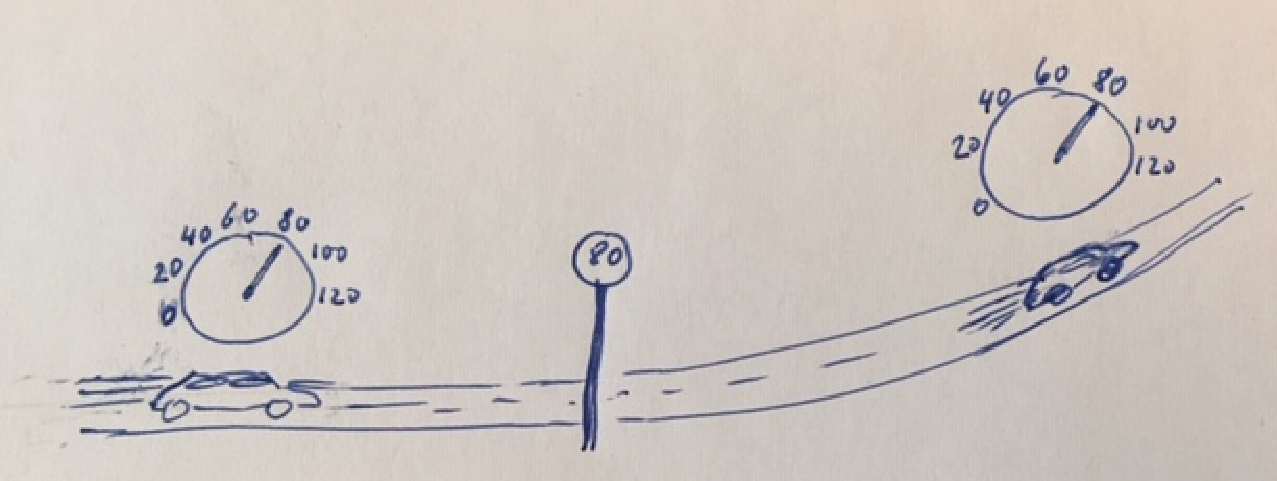
\includegraphics{motbakke}}
  \caption{En bil med {\em cruise controller} aktivert vil automatisk
    holde samme hastighet, uansett om bilen kjører rett frem eller i en motbakke. } 
  \label{fig:motbakke}
\end{figure}
For å få dette 
til blir bilens målte hastighet sammenlignet med ønsket
hastighet (som ofte er det samme for fartsgrensen), hvor forskjellen
\todo[size=\footnotesize]{Variabelnavn som brukes i figur beskrives i
  teksten, og fonten er den samme slik at leseren ser sammenhengen.}
{\tt fartsavvik} (se figur~\ref{fig:neg_feedback}) brukes av regulatoren til å
automatisk justere
{\tt bensintilførselen} (pådraget). 
\begin{figure}[H]
  \centering
  \scalebox{0.65}{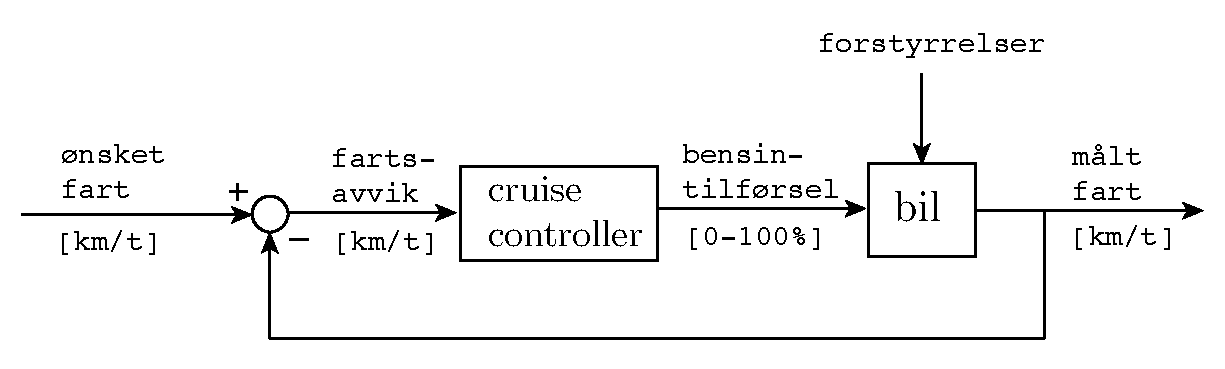
\includegraphics{neg_feedback}}
  \caption{Blokkskjema som viser prinsippet bak en {\em cruise
      controller} i en bil. Forstyrrelsene som påvirker bilen vil for
    eksempel være
  motbakke, nedoverbakke, medvind og motvind.} 
  \label{fig:neg_feedback}
\end{figure}
Dersom avviket mellom ønsket og målt fart f.eks.\ er postivt (det vil
si at ønsket fart er større enn målt fart), vil regulatoren
øke pådraget (bensintilførselen) helt til målt hastighet er lik ønsket
hastighet (og motsatt dersom avviket er negativt)\footnote{Ved kjøring uten
{\em cruise control} er det hjernen vår som utfører denne 
reguleringsfunksjonen
hvor høyrefoten justerer på gasspedalen (eller bremsen) for å oppnå ønsket hastighet.}.

Prosjektet som er beskrevet/dokumentert i dette kapittelet 
\todo[size=\footnotesize]{Eksempel på at noe er skrevet i fortid siden
  arbeidet er allerede utført.}
har gått ut på å lage 
tilsvarene funksjonalitet for turtallsregulering av LEGO-motorene. 
Dette kommer spesielt til nytte i de prosjektene hvor to motorer brukes til å
kjøre roboten fremover, 
og hvor {\em samme} pådrag blir gitt til {\em begge} motorene. Siden
motorene ikke vil møte identisk motstand/friksjon langs veien, vil man 
kunne oppleve at roboten utilsiktet svinger dersom vi ikke benytter en
turtallsregulator.


\section{Forslag til løsning}
I dette
\todo[size=\footnotesize]{Ved å bruke et par setninger i begynnelsen
  av et kapittel hvor du beskriver hva kapittelet handler om, gjør du
  leseren forberedt på innholdet.}
kapittelet presenterer vi vårt forslag til løsning av prosjektet. Dette
inkluderer en LEGO-konstruksjon som vi bygget for at 
LEGO-motoren skulle kunne utsettes for relativt lik friksjon i
forsøkene. I tillegg presenteres koden for å beregne vinkelhastighet
og koden for å implementere PID-regulatoren. 

\subsection{LEGO-konstruksjon}
For
\todo[size=\footnotesize]{Setninger som begynner med ``For å...'' gir
  hensikt og motivasjon.}
å kunne teste ut turtallsreguleringen i praksis, lagde vi
følgende LEGO-konstruksjon, se figur~\ref{fig:friksjon}. 
\begin{figure}[H]
  \centering
  \scalebox{0.5}{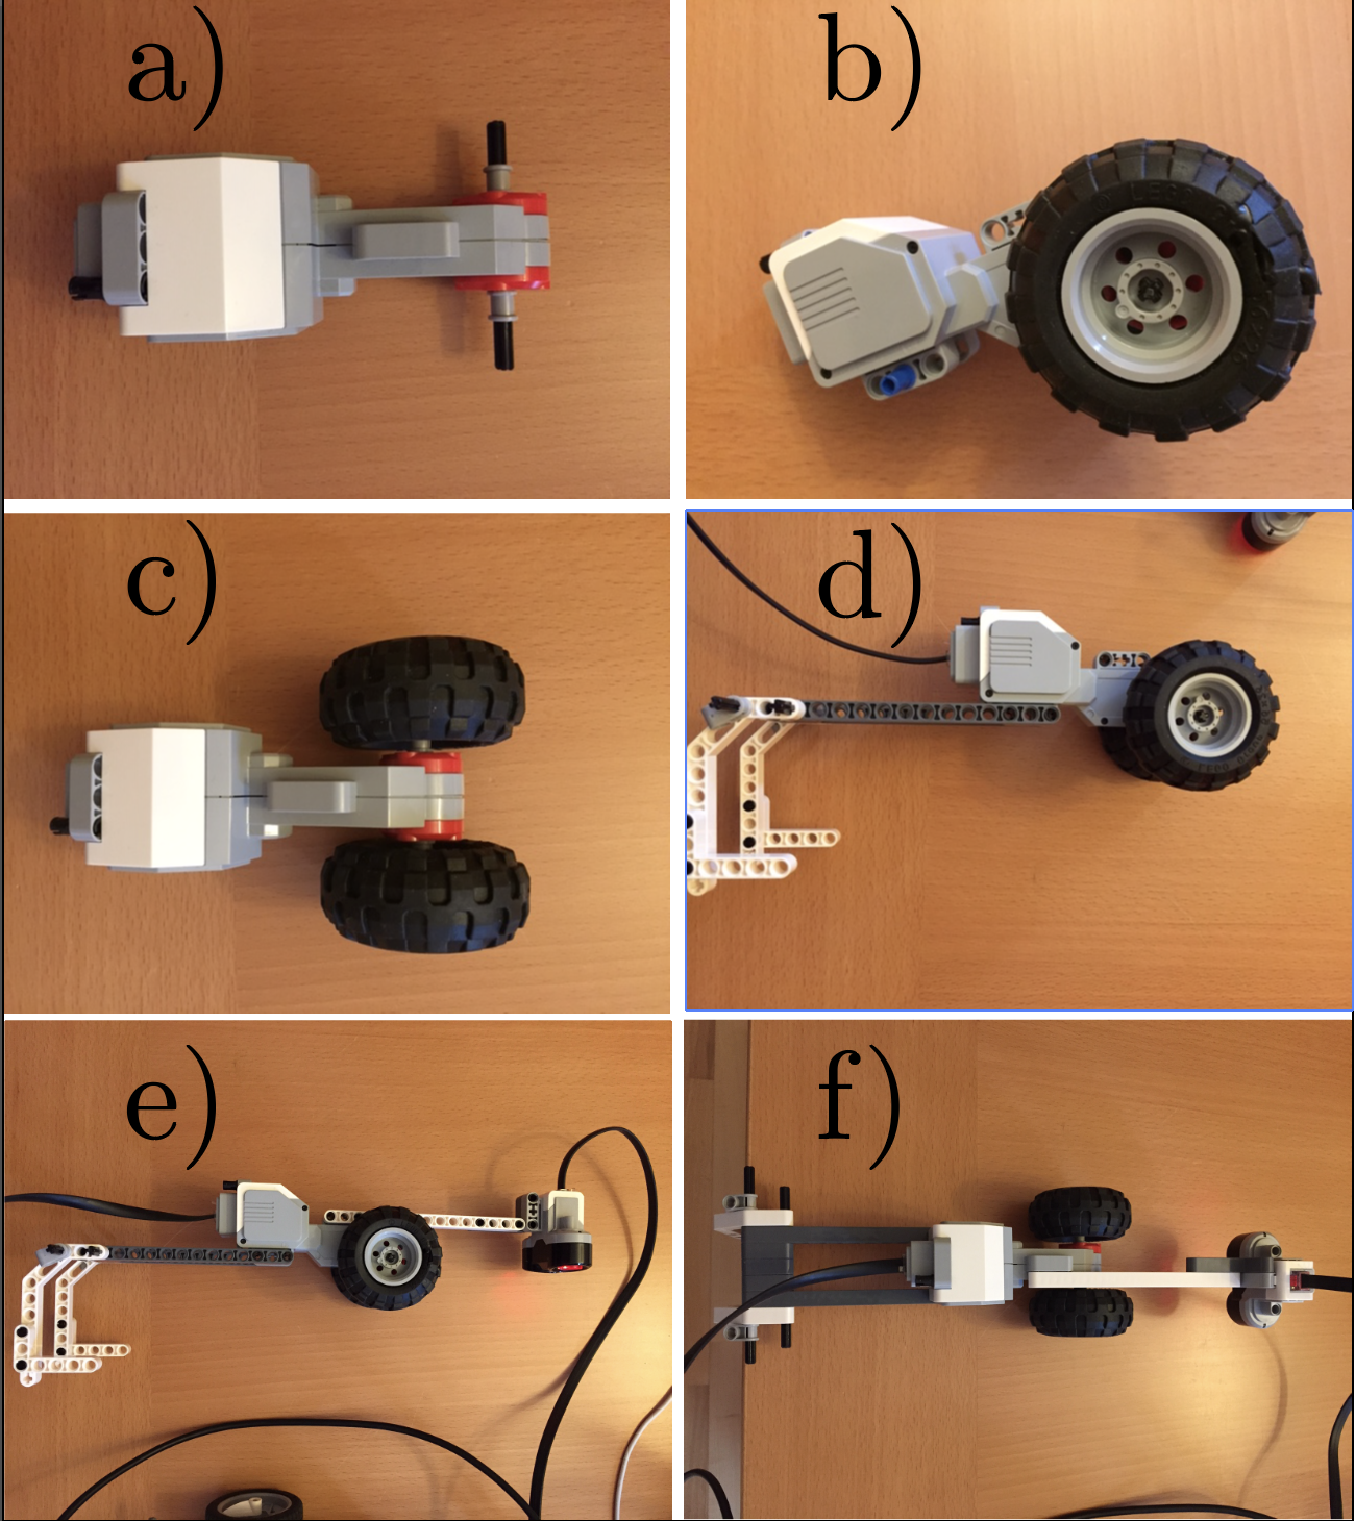
\includegraphics{friksjon2}}
  \caption{Byggebeskrivelse for repeterbart å kunne 
    tilføre noenlunde identisk friksjon på motoren.  a)~Aksling med avstandshylser
    montert. b)~og c): Hjul montert
    på begge sider av motoren. d):~Konstruksjon for å holde motoren
    igjen på bordkanten. e):~Ultralydsensor montert foran motoren for
    å registrere om konstruksjonen løftes opp fra bordet (friksjon fjernes). 
    f)~Hele konstruksjonen sett ovenfra. 
    \todo[inline,size=\footnotesize]{Figuren beskrives i caption ved å
      referere til delfigurer.} } 
  \label{fig:friksjon}
\end{figure}
Gummihjulene som er montert på motoren gjør det mulig å utsette
motoren for friksjon når hele konstruksjonen hviler mot et bord. 
Siden vekten av motoren og LEGO-delene ikke endres, er det mulig å få
relativt  like friksjonsbetingelser under forskjellige eksperiment. 

Ved å løfte på selve motoren mens den henger på bordkanten vil
friksjonen
forsvinnne. For å kunne registrere dette i datasettet,
benyttes \todo[size=\footnotesize]{
  Legg merke til at samme informasjon også
  finnes i figurteksten til figur~\ref{fig:friksjon}, men at dette
  ikke oppleves som unødvendig repetisjon.}
ultralydsensoren (som måler avstand).
Dersom motoren løftes og
kjøres uten friksjon, vil avstand til bordet bli stor. Når
konstruksjonen slippes ned på bordet, vil avstand til bordet bli
liten. 


Vi prøvde også å bruke trykkbryteren for å
\reversemarginpar\todo[size=\footnotesize]{
  Rapporten skal i hovedsak presentere løsningen som til slutt
  fungerte. Dersom flere ting har vært utprøvd, er det viktig å {\bf
    ikke} lage historiefortelling som: ``.....først så prøvde vi
  trykkbryteren....... Deretter prøvde vi
  ultralydsensoren....'', men heller først presentere det som virket,
  og deretter nevne de tingene som ikke virket og en forklaring på
  hvorfor de ikke virket.}
registrere hvorvidt konstruksjonen hviler på bordet, men denne
krevde litt for mye kraft for å bli trykket inn, og dermed oppsto det
av og til feilmålinger.


\subsection{Kode for beregning av vinkelhastighet}
I dette delkapittelet presenterer vi først koden for å styre
motorpådraget, og deretter koden for å beregne
vinkelhastigheten og turtall ut fra avlest vinkelposisjon på motoren.

For å styre en LEGO-motor (som ikke er turtallsregulert) 
settes pådraget til
en verdi på mellom $-100$ og $100$. Dette tallet kan tolkes til å ha
enheten~[\%], hvor positivt verdi roterer ``fremover'', mens negativt tall roterer
``bakover''.
I uttestingsfasen av turtallsregulatoren
benyttet vi {\em potensiometeret}
(se figur~\ref{fig:potmeter})
\reversemarginpar\todo[size=\footnotesize]{Figur~\ref{fig:potmeter}
  kommer på toppen av neste side  
  siden vi på denne figuren bruker [ht] istendenfor [H], se
  {\LaTeX}-koden i chapter6.tex.}
som pådrag til motoren.
Dette fordi vi på denne måten
kunne holde pådraget helt konstant/fast over en tidsperiode, men
samtidig at det var enkelt å justere nivået på pådraget i
samme eksperiment (som et sprang)\footnote{Alternativt kunne
vi benyttet selve styrestikken, men denne er det 
vanskelig å holde i en konstant posisjon. }. 
Kodeutdraget under viser hvordan
avlest potensiometerverdi
\reversemarginpar\todo[size=\footnotesize]{I beskrivelsen av koden er det viktig at
  variabelnavn skrives i samme font (gir gjenkjenning) og at det
  hjelper leseren dersom du angir linjenummer. }
{\tt  PotMeter(k)} (linje 1) benyttes direkte som 
pådragsverdi til motor A, {\tt PowerA(k)} (linje 2). De to siste
kommandolinjene starter motor A.
\normalmarginpar\todo[size=\footnotesize]{Hele kodeutdraget består av
  kodelinjer hentet fra  filene 
{\tt  P08\_F3\_....} og 
{\tt  P08\_F5\_...} og er presentert på en kompakt måte for leseren.}
\begin{lstlisting}[caption=Kode for å bestemme
og sette pådraget til motor A
  (Mac-versjon), 
  label=kode:padrag]
  PotMeter(k) = -skalering*axis(joystick,4);
  PowerA(k) = PotMeter(k);
  motorA.Speed = PowerA(k);
  start(motorA);   
\end{lstlisting}

\begin{figure}[ht] % plasseres nær her og i topp 
  \centering
  \scalebox{0.4}{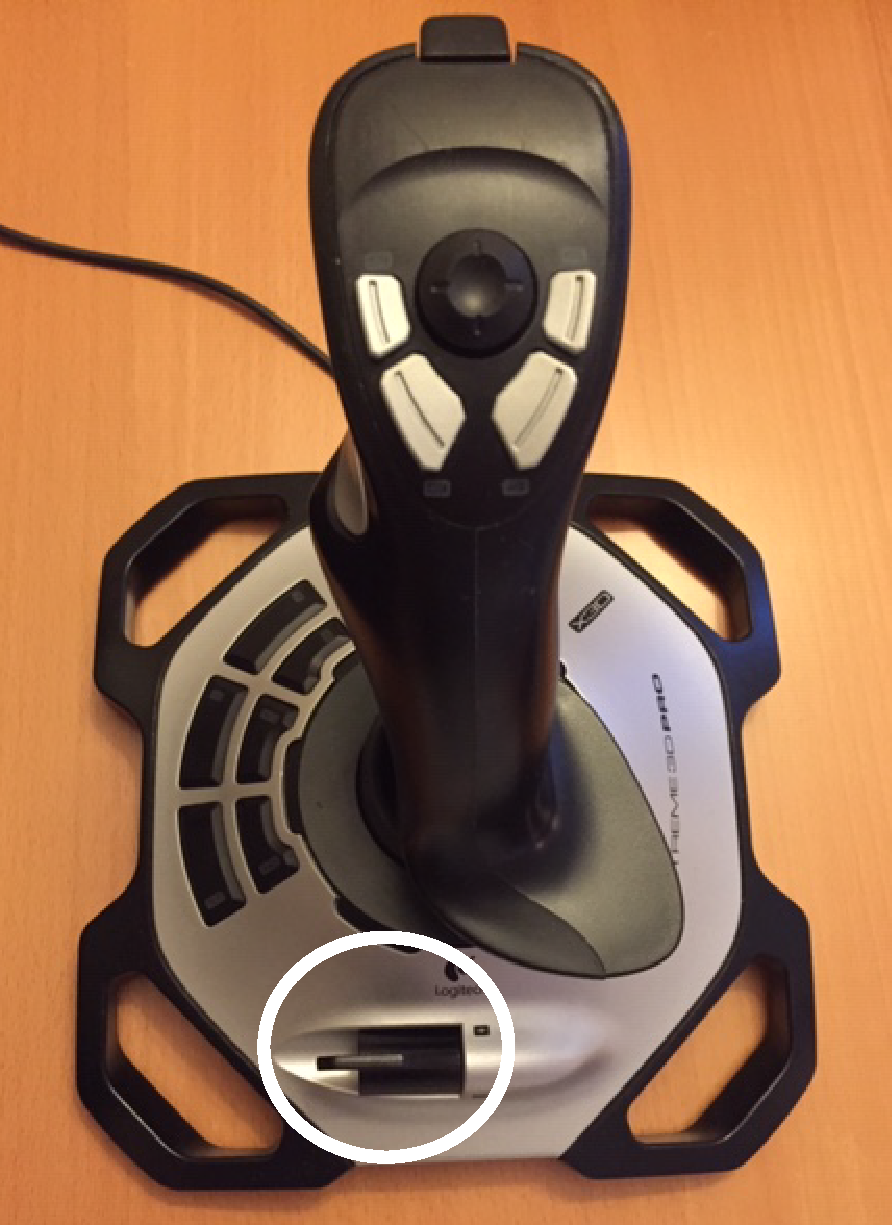
\includegraphics{potmeter}}
  \caption{Potensiometeret indikert med hvit ring benyttes som pådrag til
    motoren.} 
  \label{fig:potmeter}
\end{figure}

Prinsippet bak å beregne vinkel\-hastigheten (i enheten [grader/s])
er å først avlese vinkelposisjonen til motor A (i enheten [grader]) og
deretter derivere denne ved hjelp av derivasjonsfunksjonen fra 
kapittel~\ref{kap:derivasjon}. Siden 
vinkelposisjonsmålinger er befengt med støy (vil gi ubrukelig resultat
etter derivering), så blir 
disse først filterert. Kodeutdrag~\ref{kode:vinkelHast} viser
nødvendig kode,
\begin{lstlisting}[caption=Kode for beregning av vinkelhastighet til
  motor A., label=kode:vinkelHast, firstnumber=5]
VinkelPosA(k) = double(motorA.readRotation);
alfa1 = 0.3;
VinkelPosA_IIR(k) = IIR_filter(VinkelPosA_IIR(k-1),VinkelPosA(k),alfa1);
VinkelHastA(k-1) = Derivation(VinkelPosA_IIR(k-1:k), Ts(k-1));
\end{lstlisting}
hvor
\begin{itemize}
  \setlength\itemsep{-1mm}
\item {\tt  VinkelPosA(k)} i linje 5 er avlest vinkelposisjon.
  \item Verdien på {\tt alfa1=0.3} i linje 6 ble funnet etter endel prøving og
    feiling.
\item {\tt  VinkelPosA\_IIR(k)} i linje 7 er filtrert vinkelposisjon.
\item {\tt  VinkelHastA(k-1)} i linje 8 er beregnet vinkelhastighet.
\end{itemize}

Oppsummert kan det som skjer i
kodeutdragene~\ref{kode:padrag} og \ref{kode:vinkelHast} presenteres som
blokkskjemaet i delfigur a) figur~\ref{fig:open_sloyfe}. Delfigur b)
er en komprimert versjon som vi gjenbruker senere når vi presentererer
turtallsregulatoren. 
\begin{figure}[H]
  \centering
  \scalebox{0.65}{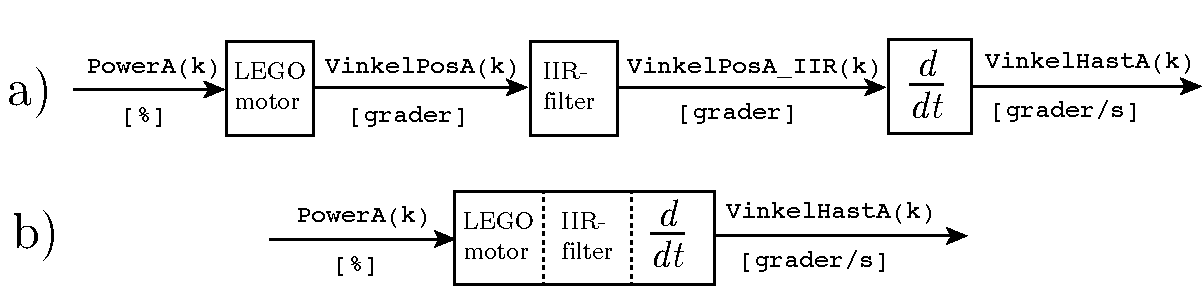
\includegraphics{open_sloyfe}}
  \caption{a): Blokkskjema over koden i
    kodeutdragene~\ref{kode:padrag} og \ref{kode:vinkelHast}. b):~En komprimert fremstilling av
    blokkskjemaet i a). } 
  \label{fig:open_sloyfe}
\end{figure}

\subsection{Testing uten turtallsregulator}
For å finne uten hvordan LEGO-motoren håndterte friksjon uten
turtallsregulator, gjennomførte vi et eksperiment 
hvor konstruksjonen i figur~\ref{fig:friksjon} ble løftet opp og lagt
ned igjen på bordet ved forskjellige pådrag. Et typisk resultat er
vist i  figur~\ref{fig:hastighet_uten}.

I dette eksperimentet
ble det benyttet 3 forskjellige pådrag,
markert med $i$, $ii$ og $iii$ i delfigur~a). Midt i tidsperioden for 
hver av de tre pådragene 
ble LEGO-konstruksjonen løftet opp, og dette er
markert med røde ringer i delfigur~d).
 Når LEGO-konstruksjonen ligger på bordet er avstanden målt med
 ultralydsensoren ca
 4~cm.

 Delfigur~b) viser målt vinkelposisjon (IIR-filtrert), og siden motoren
roterer samme vei gjennom hele eksperimentet, øker denne monotont. Det kan
observeres at økning er størst i de periodene hvor LEGO-konstruksjonen
er løftet opp fra bordet
(market med piler).
I løpet av
eksperimentet som varer ett minutt, har motoren roteret 
\todo[size=\footnotesize]{I teksten vises det tydelig til detaljer i
  figuren slik at leseren slipper å lete i figuren etter det som
  beskrives. Poenget med ligning (6.1) er bare for å relatere
  tallverdien til noe leseren har et forhold til, og fungerer kanskje mer som {\em fun fact}.}
ca $2.2{\cdot}10^{4}$ grader, noe som tilsvarer
\begin{equation}
  \label{eq:1}
  \frac{22000}{360} \approx 60 \mathrm{~runder}
\end{equation}

\newpage
\hspace*{0mm}\todo[size=\footnotesize]{Legg merke til at figuren har tydelige og
  lesbare akseverdier, at aksene har tydelig benevning og titler som
  beskriver hva som vises, at det inkluderes piler, tekst, sirkler og
  andre elementer for å tydeliggjør sammenhenger. Dette forenkler også
  mulighetene til å beskrive resultatene i rapportteksten.}
\begin{figure}[H]
  \centering
  \hspace*{-10mm}\scalebox{0.93}{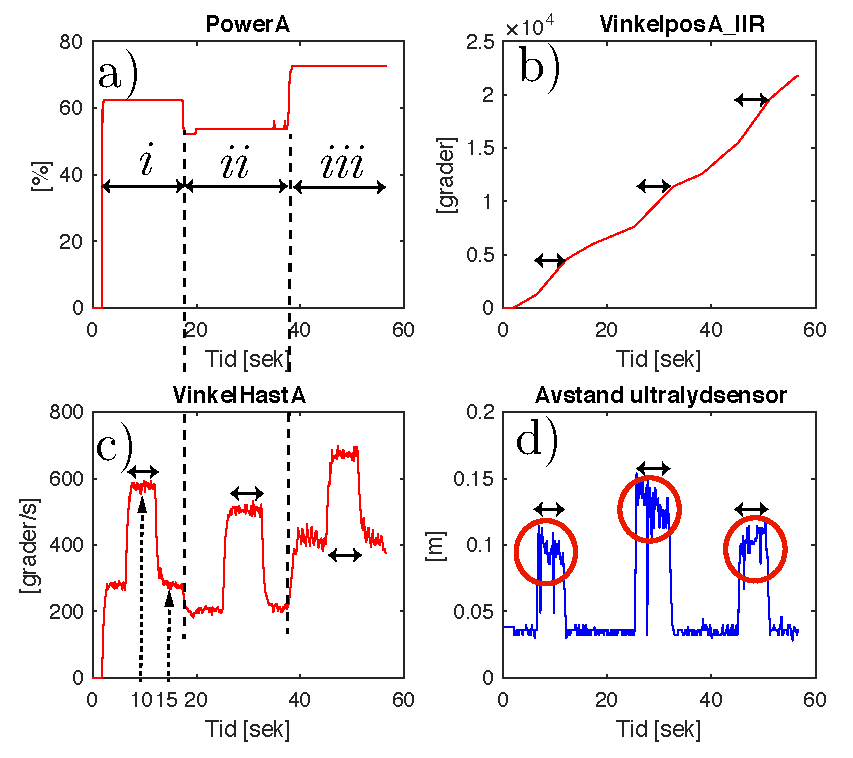
\includegraphics{hastighet_uten}}
  \caption{Målinger og beregninger fra et eksperiment som viser
    hvordan friksjon endrer vinkelhastigheten på en
    LEGO-motor uten turtallsregulator. a):~Pådragsverdier til LEGO-motoren, delt
    inn i perioder markert med $i$, $ii$ og $iii$ hvor pådraget er
    forskjellig, men konstant.
    b):~Filtrert vinkelposisjon til
    motor A. c):~Beregnet vinkelhastighet ut fra
    de filtrerte målingene i~b). d):~Målinger fra
    ultralydsensoren hvor periodene indikert med rød ring betyr at
    LEGO-konstruksjonen i figur~\ref{fig:friksjon} er løftet opp fra
    bordet. } 
  \label{fig:hastighet_uten}
\end{figure}

Delfigur~c) viser den beregnede vinkelhastigheten i [grader/s], og
vi ser at vinkelhastigheten halveres når LEGO-konstruksjonen hviler på
bordet. Dette kan f.eks. ses ved de loddrette pilene ved tidspunkt
\todo[size=\footnotesize]{Ved første øyekast i
  delfigur c) ser du kanskje ikke at vinkelhastigheten halveres, men
  ved å indikere tidspunkt og bruke piler (eller annet) hjelper du
  leseren til å forstå resonnementet.}
$t{=}10$ og $t=15$ sekund, hvor  
vinkelhastigheten først er ca 600 grader/s (tilsvarer at roboten er løftet
opp, se delfigur d)), og etter at roboten legges ned på bordet 
reduseres vinkelhastighet til  ca 300 grader/s.


\subsection{Sammenheng mellom pådrag og vinkelhastighet}
Som vist i eksempelet med
 {\em cruise controlleren} i 
figur~\ref{fig:neg_feedback}, så føres {\em målingen} 
\fbox{\tt målt fart} tilbake og sammenlignes 
med {\em referansen} \fbox{\tt ønsket fart}. Sammenligningen
innebærer en subtraksjon og beregning av {\em reguleringsavviket} 
\fbox{\tt fartsavvik} som
\begin{equation}
  \label{eq:3}
  \mathtt{fartsavvik}=
  \mathtt{onsket~fart}-\mathtt{malt~fart}
\end{equation}
En forutsetning for å beregne dette avviket er lik benevningen 
for referanse og måling, i dette tilfelle [km/t].
På tilsvarende måte må referansen for
turtallsregulatoren, \todo[size=\footnotesize]{Ved å ramme inn
  variabelnavn tydeliggjør du symbolbruken som vises i figuren.}
 \fbox{\tt ønsket vinkelhastighet}, ha samme
benevning som \fbox{\tt målt vinkelhastighet}, dvs.\ [grader/s]. Dette er illustrert
i figur~\ref{fig:neg_feedback_vinkel} hvor vi har tatt utgangspunkt i
det komprimerte blokkskjema fra delfigur b) i
figur~\ref{fig:open_sloyfe} og vist hvordan det prinsipielle
blokkskjema for turtallsregulatoren vil se ut.
\begin{figure}[H]
  \centering
  \hspace*{-10mm}\scalebox{0.6}{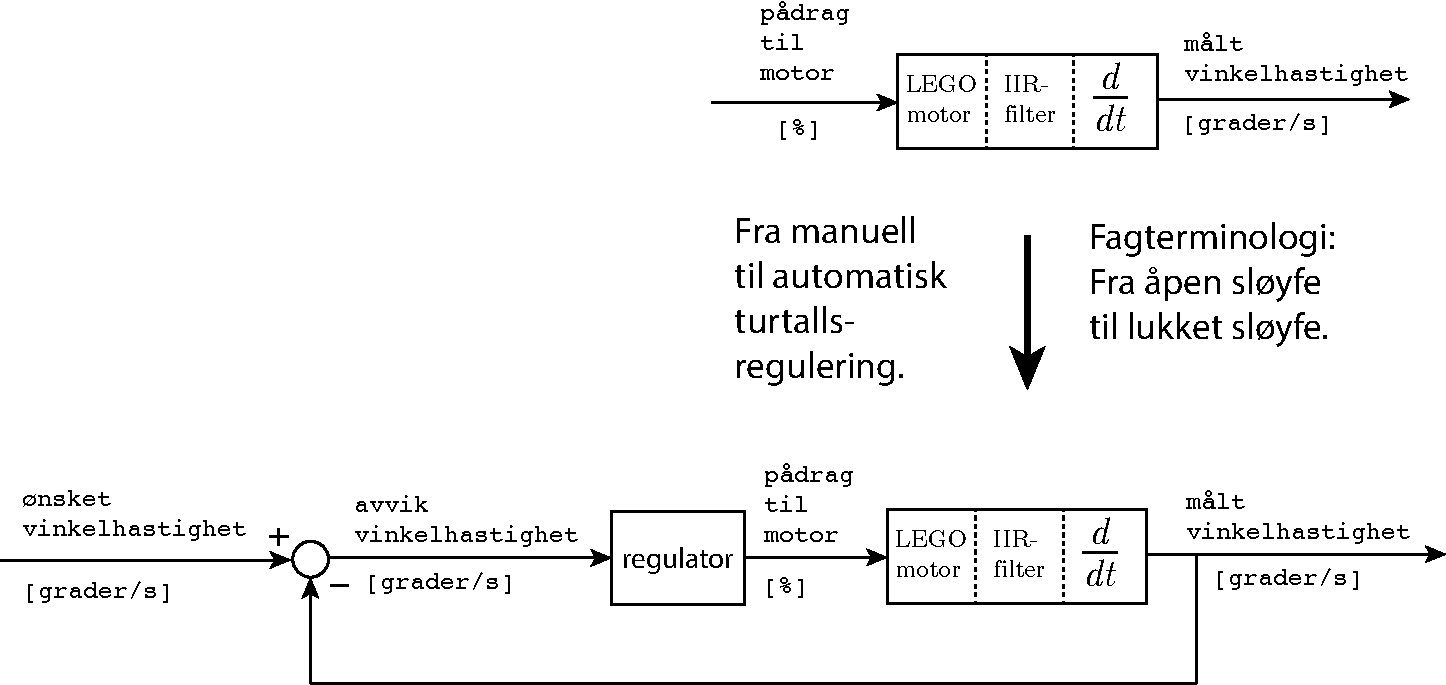
\includegraphics{neg_feedback_vinkel}}
  \caption{Blokkskjema som viser hvordan LEGO-motoren fra
    delfigur b) i figur~\ref{fig:open_sloyfe} 
    må kobles opp
    for å gå fra manuell til automatisk
    turtallsregulering. Reguleringsteknisk fagterminologi er fra åpen
    sløyfe til lukket sløyfe.} 
  \label{fig:neg_feedback_vinkel}
\end{figure}

For at vi skulle kunne
spesifisere oppnåelige verdier i \fbox{\tt ønsket vinkelhastighet},
måtte vi derfor først finne {\bf maksimalt} oppnåelig vinkelhastighet på
LEGO-motoren.  Dette ville da 
være øvre\footnote{Og tilsvarende nedre med motsatt fortegn.}
grense for referansen.
Vi gjennomførte derfor et forsøk hvor vi rolig økte pådraget til
motoren fra $-100$\% til $+100$\%, uten at vi tilførte friksjon på  motoren. 
Resultatet fra dette forsøket er vist i
figur~\ref{fig:power_vs_turtall}, hvor delfigur a)  viser pådraget
\fbox{\tt PowerA} som
funksjon av tid, delfigur b) viser beregnet vinkelhastighet 
\fbox{\tt  VinkelHastA}, og
delfigur c) viser sammenhengen mellom pådrag og vinkelhastighet, dvs.\
\fbox{\tt  VinkelHastA} som funksjon av \fbox{\tt PowerA}. 
\begin{figure}[H]
  \centering
  \hspace*{-10mm}\scalebox{0.9}{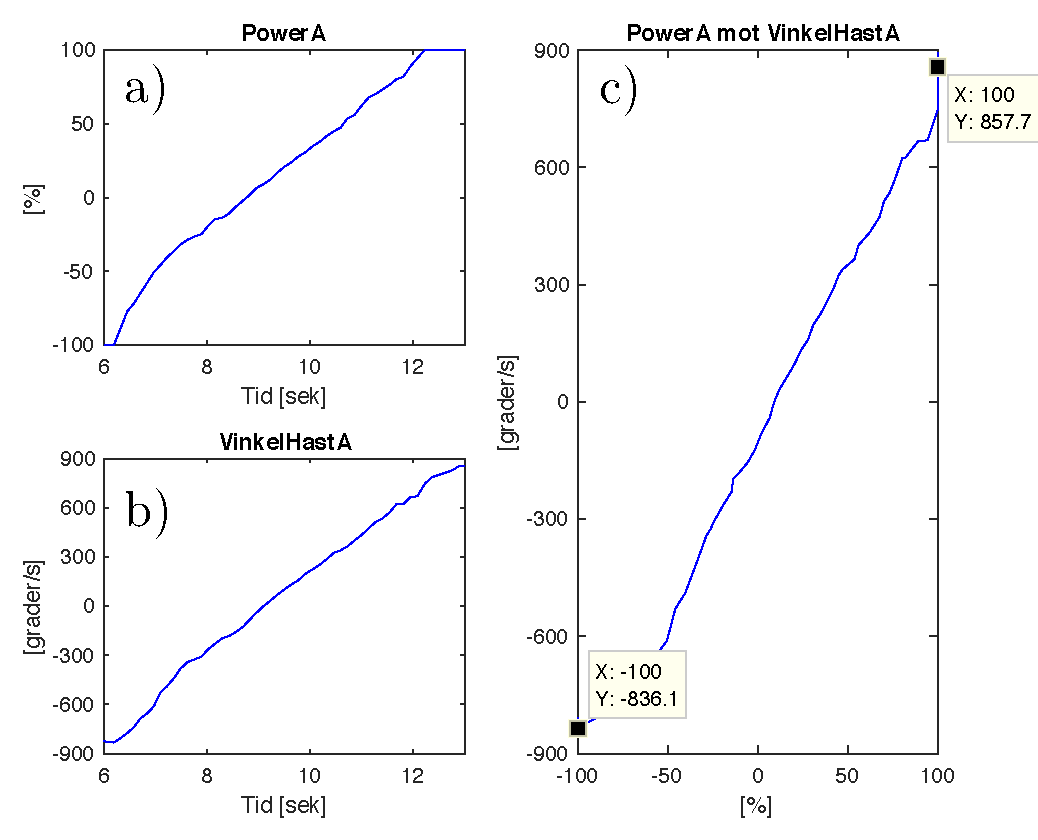
\includegraphics{power_vs_turtall}}
  \caption{Resultater som viser sammenheng mellom {\tt PowerA} og
    beregnet vinkelhastighet  {\tt VinkelHastA}. a): {\tt PowerA} som
    funksjon av tid. b): {\tt VinkelHastA} som funksjon av tid. c):
    {\tt VinkelHastA} som funksjon av {\tt PowerA}. } 
  \label{fig:power_vs_turtall}
\end{figure}

Som vi kan se fra avlesningen i delfigur c), gir fullt positivt pådrag på motoren en
vinkelhastighet på ca 857 [grader/s], men fullt negativt pådrag gir en
vinkelhastighet på ca -836 [grader/s]. For å unngå {\em
  windup}-problemer i reguleringen (se nedenfor), avrunder vi nedover
og bestemmer at maksimal oppnåelig vinkelhastighet (uten friksjon) er $\pm 800$~[grader/s], dvs.
\begin{align}
  \mathtt{PowerA}&\mathtt{=\pm 100~[\%]} \notag \\
  &\downarrow \notag \\
  \mathtt{VinkelHastA}&=\mathtt{\pm 800~[grader/s]} \notag
\end{align}
Dette innebærer at den prinsipielle reguleringssløyfen i
figur~\ref{fig:neg_feedback_vinkel}
kan presenteres med mer detaljer som vist i
delfigur a) i figur~\ref{fig:reg_sloyfe1}. Legg merke til at
referansen\footnote{Referansen kalles også 
{\em settpunkt} eller {\em skal-verdi}.}
kalles \fbox{\tt Ref\_VinkelHastA}, siden målingen 
kalles \fbox{\tt VinkelHastA}.

\begin{figure}[H]
  \centering
  \hspace*{-15mm}\scalebox{0.65}{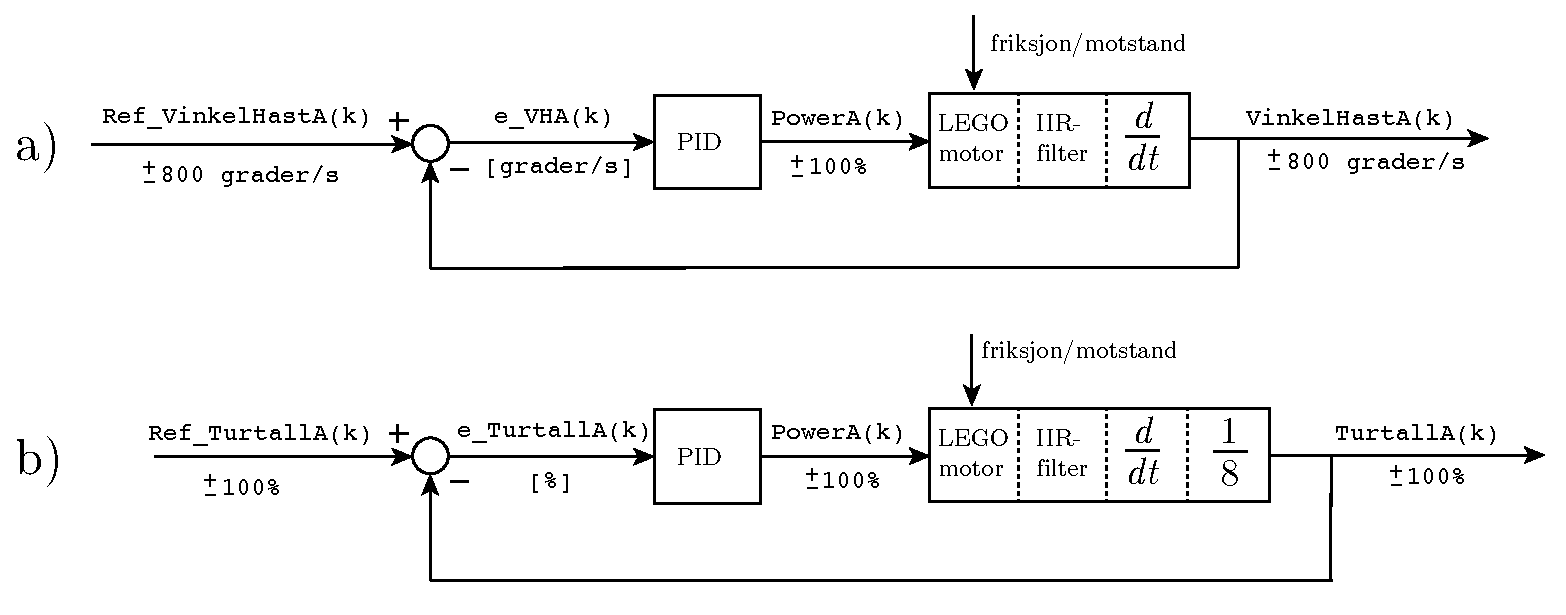
\includegraphics{reg_sloyfe1}}
  \caption{a): Blokkskjema over turtallsregulatoren hvor verdiene til 
    referansen \fbox{\tt Ref\_VinkelHastA} varierer mellom $\pm
    800$~grader/s. b): Blokkskjema over turtallsregulatoren hvor verdiene til 
    den relative referanse \fbox{\tt Ref\_TurtallA} varierer mellom $\pm
    100$~\%. Legg merke til at friksjon/motstand er tegnet inn som en
    forstyrrelse på motorblokken.
    \todo[inline,size=\footnotesize]{Det gjør ingenting om figurene
      dine bruker margene på begge sider, dersom dette trengs for å
      gjøre de lesbare.}} 
  \label{fig:reg_sloyfe1}
\end{figure}
For å forenkle bruken av turtallsregulatoren fant vi ut at det å
normalisere vinkelhastigheten til en verdi mellom $\pm100$~\% gjorde
det mye enklere å bytte mellom manuell og automatisk kjøring siden vi
da slapp å måtte forholde oss til følgende veldig forskjellige benevninger:\\[-7mm]
\begin{itemize}
\setlength\itemsep{-1mm}
\item pådrag i [\%] ved manuell kjøring av motoren og, 
\item ønsket vinkelhastighet i [grader/s] ved automatisk kjøring
\end{itemize}

Ved å normalisere
vinkelhastigheten med det absolutte variasjonsområdet
$\pm800$~grader/s til et generelt 
\fbox{turtall} med det relative variasjonsrområdet
$\pm100$~\%, vil selve {\em verdien} vi forholder oss til i manuell og
automatisk kjøring være identisk. Det betyr altså at 
variasjonsområdet til pådraget/referansen vil være
identisk, og forskjellen vil være hvorvidt
turtallsregulatoren er aktiv eller ikke.



Strukturen for denne turtallsregulatoren er vist i
delfigur~b) i figur~\ref{fig:reg_sloyfe1}, hvor vi har lagt til en
skaleringsblokk på $\frac{1}{8}$ etter derivasjonsrutinen. 
Siden denne nye måleverdien
representerer den generelle størrelsen 
turtall i [\%], har vi endret utgangen og
referansen til henholdsvis \fbox{\tt TurtallA} og 
\fbox{\tt  Ref\_TurtallA}. Koden for å beregne {\tt TurtallA} baserer
seg da på kodeutdrag~\ref{kode:vinkelHast} i tillegg til 
følgende kode:
\begin{lstlisting}[caption=Kode for å beregne {\tt TurtallA}.,
  label=kode:rotHast, firstnumber=9]
TurtallA(k-1) = 1/8*VinkelHastA(k-1);
\end{lstlisting}

Koden i dette kapittelet er plassert i {\tt
  P0X\_F4\_MathCalculations.m}.
\todo[size=\footnotesize]{Legg merke til at vi ikke viser koden for
  ultralydsensoren som registrerer om LEGO-konstruksjonen løftes
  opp. Dette fordi dette ikke er en viktig del av selve turtallsregulatoren.}




\subsection{Kode for turtallsregulator}
I dette delkapittelet blir koden for turtallregulatoren
presentert. Den er basert på en standard industriell PID-regulator som 
matematiske kan uttrykkes som i
ligning~\eqref{eq:10a},
\begin{align}
 u(t) =&  u_{0} + \underbrace{K_P{\cdot} e(t)} + 
             \underbrace{K_{I}\int_0^t e(t)dt} + 
             \underbrace{K_D {\cdot}\frac{d}{dt} e_{f}(t)}   \label{eq:10a}\\
 & \hspace*{14mm} \mathrm{P} \hspace*{20mm} \mathrm{I} 
\hspace*{22mm} \mathrm{D} \notag
\end{align}
hvor 
\begin{itemize}
\setlength\itemsep{0mm}
\item $u_{0}$ er basispådraget som for turtallsregulatoren
  er satt lik 0.
\item $e(t)$ er reguleringsavviket som er forskjell mellom referansen
  og målingen
\item $e_{f}(t)$ er filtrert reguleringsavvik
\item $K_{P}$, $K_{I}$ og $K_{D}$ er regulatorparametre.  
\item $u(t)$ er det beregnede totalpådraget 
\item Bokstavene $\mathrm{P}$, $\mathrm{I}$ og  
 $\mathrm{D}$ står for henholdsvis proporsjonaldel, integraldel og
  derivat\-del. 
\end{itemize}

For å relatere disse generelle variablene og parametrene 
til turtallsregulatoren vist
som en PID-blokk i  figur~\ref{fig:reg_sloyfe1}b). 
kan ligning~\eqref{eq:10a} skjematisk presenteres som
figur~\ref{fig:pid_blokk}.
\begin{figure}[H]
  \centering
  \hspace*{0mm}\scalebox{0.65}{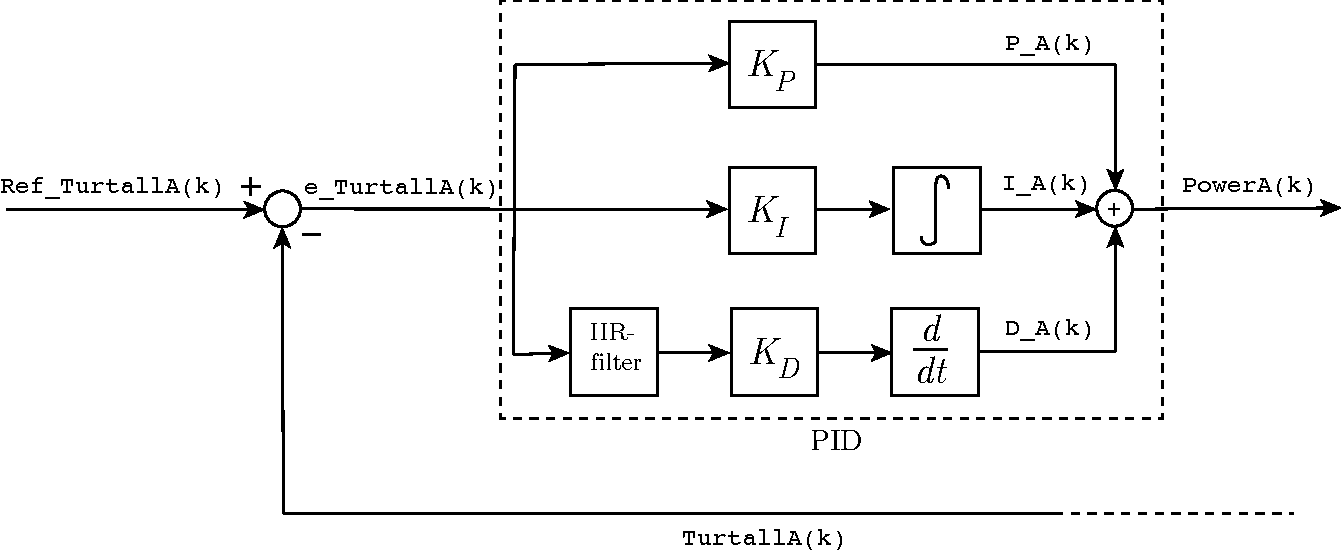
\includegraphics{pid_blokk}}
  \caption{Blokkskjema over turtallsregulatoren vist som PID-blokk i
    figur~\ref{fig:reg_sloyfe1}b) og som er basert på
    ligning~\eqref{eq:10a}. Bidragene {\tt P\_A(k)},  {\tt I\_A(k)} og  
    {\tt D\_A(k)}  tilsvarer bidragene $\mathrm{P}$, $\mathrm{I}$ og  
    $\mathrm{D}$ i ligning~\eqref{eq:10a}.} 
  \label{fig:pid_blokk}
\end{figure}
Detaljer om koden for turtallsregulatoren er som følger:

\begin{itemize}
\setlength\itemsep{0mm}
\item
  Reguleringsavviket {\tt e\_TurtallA(k)}  beregnes først som differansen
  mellom {\tt Ref\_TurtallA(k)} (som settes lik potensiometerposisjonen 
  fra kode~\ref{kode:padrag}) og beregnet
  turtall {\tt TurtallA(k-1)} fra
  kode~\ref{kode:rotHast}. Dette er vist i kode~\ref{kode:e_RHA}.
\begin{lstlisting}[caption=Beregning av reguleringsavviket {\tt e\_TurtallA(k)}., 
  label=kode:e_RHA, firstnumber=15]
  Ref_TurtallA(k) = PotMeter(k)
  e_TurtallA(k) = Ref_TurtallA(k) - TurtallA(k-1);
\end{lstlisting}
Legg merke til at vi antar at beregnet turtall i forrige
tidsskritt {\tt k-1} kan brukes til å beregne et avvik i nåværende
tidsskritt {\tt k}.

\item Proporsjonaldelen {\tt P\_A(k)} forsterker
  reguleringsavviket med
  parameteren $K_{P}$, se kodeutdraget under. 
\begin{lstlisting}[caption={Beregning av P-delen for motor A, {\tt P\_A(k)}.}, 
  label=kode:P_del, firstnumber=17]
  P_A(k) = Kp*e_TurtallA(k);
\end{lstlisting}
  Dersom avviket {\tt e\_TurtallA(k)=0},  som jo egentlig er det vi ønsker å
  oppnå, vil proporsjonaldelen også bli 0.  

\item Integraldelen {\tt I\_A(k)} integrerer produktet av reguleringsavviket og 
  integrasjonsforsterkningen $K_{I}$, se kodeutdraget under. 
\begin{lstlisting}[caption={Beregning av I-delen  for motor A {\tt I\_A(k)}.}, 
  label=kode:I_del, firstnumber=18]
  I_A(k) = EulerForward(I_A(k-1), Ki*e_TurtallA(k-1), Ts(k-1));
\end{lstlisting}
Til dette bruker
vi integrasjonsfunksjonen {\tt EulerForward} fra kapittel~\ref{kap:prosjekt01}.

\item Derivatdel {\tt D\_A(k)} deriverer produktet mellom det
  IIR-filtrerte reguleringsavviket og
  derivasjonsforsterkningen $K_{D}$, se under. 
\begin{lstlisting}[caption={Beregning av D-delen for motor A, {\tt D\_A(k)}.}, 
  label=kode:D_del, firstnumber=19]
  e_TurtallA_IIR(k) = IIR_filter(e_TurtallA_IIR(k-1), e_TurtallA(k), alfa2);
  D_A(k) = Derivation(Kd*e_TurtallA_IIR(k-1:k), Ts(k-1));
\end{lstlisting}
Til dette bruker vi funksjonen {\tt Derivation} fra
kapittel~\ref{kap:derivasjon}, med en $\alpha$-verdi {\tt alfa2}.

\item Totalpådraget {\tt PowerA}(k) beregnes til slutt 
  som summen av alle delpådragene
  som vist i koden under
  \begin{lstlisting}[caption=Kode for totalpådraget {\tt PowerA(k)} for motor A., 
    label=kode:PID, firstnumber=21]
    PowerA(k) = P_A(k)+I_A(k) + D_A(k);
  \end{lstlisting}
  I uttestingen av turtallsregulatoren, plottet vi alle
  bidragene {\tt P\_A(k)},  {\tt I\_A(k)} og  {\tt D\_A(k)}  i figurer
  slik at vi fikk innsikt i hvordan regulatoren fungerte.
\end{itemize}

Koden i dette kapittelet er plassert i {\tt P0X\_F5\_CalculateAndSetMotorPower.m}.

\newpage

\section{Resultat}
I dette kapittelet blir resultatene fra testing av turtallsregulatoren
presentert. Først presenteres resultatene for P-regulatoren med dens 
begrensinger. Deretter presenteres resultatene for PI-regulatoren og vi
dokumenterer behovet for integratorbegrensing. Til slutt presenteres 
resultatene for PID-regulatoren.
%, samt effekten av å justere de
%forskjellige regulatorparametre $K_{P}$, $K_{I}$ og $K_{D}$.

Resultatene består av tidsresponskurver som viser hvordan de forskjellige
regulatorene klarer å opprettholde turtallet når LEGO-konstruksjonen
blir løftet opp og ned fra bordet (på tilsvarende måte som vist i 
figur~\ref{fig:hastighet_uten}). 
For å stille inn regulatorene brukte vi prøve-og-feile metoden.


\subsection{P-regulator}
Den enkleste regulatoren er en P-regulator, og den består kun av koden
vist i kodeutdrag~\ref{kode:P_del}. De beste resultatetene oppnådde vi
ved å bruke {\tt alfa=0.3} og {\tt Kp=1}, og et eksempel på en kjøring
er  vist i figur~\ref{fig:P_reg}. 
Som vi ser fra delfigur b), klarer ikke P-regulatoren å 
følge referansen siden lengden på dobbelpilene markert med røde ringer indikerer hvor stort
reguleringssavviket \fbox{\tt e\_TurtallA} er. I tidspunktet rundt den
første røde ringen ($t{\approx}12$~sekund) ligger motoren ned mot
bordet og utsettes for friksjon som vist i delfigur
d). Reguleringssavviket avlest i b) ved $t{\approx}12$~sekund er ca 
\begin{equation}
  \label{eq:5}
  \mathtt{e\_{TurtallA}}\approx 65\%- 20\% = 45\%
\end{equation}

Den avleste pådragsverdien fra P-delen 
i c) ved samme tidspunkt er ca 45\% (første røde ringen). 
Dette  stemmer med uttrykket for en P-regulator når {\tt Kp=1}: 
\begin{align}
  \mathtt{P\_{A}} & = \mathtt{Kp} \cdot \mathtt{e\_{TurtallA}} \label{eq:p_reg}\\
                          & =  45
\end{align}
En viktig observasjon fra ligning~\eqref{eq:p_reg} som er gyldig for
P-regulatorer i sin alminnelighet er at for å oppnå et pådrag som i
det hele tatt er større enn 0, må reguleringsavviket også være større
enn 0.  Eller sagt med ord: Det må være
avvik mellom ønskelig og virkelig turtall for at motoren i
det hele tatt skal rotere.

\begin{figure}[H]
  \centering
  \hspace*{0mm}\scalebox{0.88}{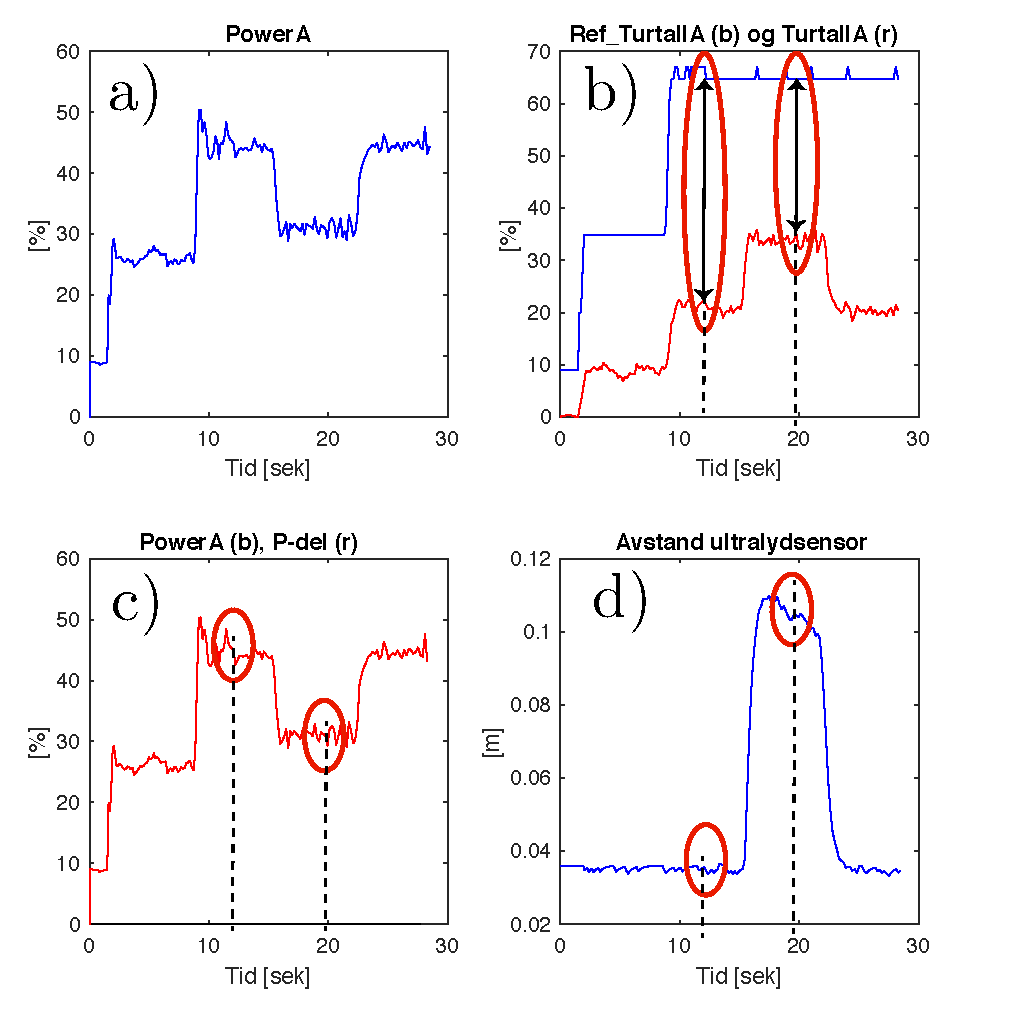
\includegraphics{P_reg}}
  \caption{Målinger og beregninger fra et eksperiment som viser
    at P-regulatoren ikke klarer å følge referansen, verken med eller
    uten friksjon. Følgende
    parametre ble benyttet: {\tt alfa1=0.3}, {\tt Kp=1}, {\tt Ki=0},
    {\tt Kd=0}.
    a):~Beregnede pådragsverdier fra P-regulatoren. 
    b):~Referanse fra potensiometerert (blått) og beregnet
    turtall [\%] (rødt). 
    c):~Bidragene fra P-del (rødt) og totalpådraget {\tt
      PowerA} (blått). 
    d):~Avstandsmålinger fra ultralydsensoren.
    Forklaring
    til resultatene er gitt i teksten.} 
  \label{fig:P_reg}
\end{figure}


Når LEGO-konstruksjonen
løftes opp fra bordet ved $t{\approx}20$~sekund som vist i d),
reduseres reguleringssavviket til $\mathtt{e\_TurtallA}{\approx}30$. 
Årsaken til dette er at når 
friksjonen forsvinner så roterer motoren lettere og 
turtallet øker (rød kurve i b)).  
Konsekvensen er altså at reguleringsavviket 
reduseres (kortere dobbelpil i b)), men dermed reduseres også pådraget
(rød kurve i c)).  Denne oppførselen stemmer med ligning~\eqref{eq:p_reg}.

For å oppsummere, så viser resultatene 
at en P-regulator ikke er i stand til å holde
motorturtallet på en gitt referaseverdi, verken når den er påvirket eller
upåvirket av friksjon. Ved å øke verdien av {\tt Kp} vil
reguleringsavviket reduseres, men det vil aldri bli lik 0 som vi egentlig
ønsker. For å få fjernet reguleringsavviket må vi benytte en
PI-regulator, se neste delkapittel.

\subsection{PI-regulator}
Ved å gjennomføre et lignende eksperiment som for P-regulatoren, fikk vi 
resultatene vist i figur~\ref{fig:turtallregulering}, hvor
{\tt alfa1=0.3}, {\tt Kp=1} og {\tt Ki=2}. Resultatene
er delt inn i tidsperiodene  $i$ og $ii$ som markerer to
forskjellige referanseverdier, se blå kurve i b). 

For å beskrive funksjonen til en PI-regulator, henvises det til
tidsperiode $ii$. 
Når LEGO-konstruksjonen er løftet opp fra bordet, 
indikert med rød ring i~d), er totalpådraget i~a) ca 45\%  samtidig som både
turtallet og referanseverdien i b) på ca 50\%. 
Dette betyr  at regulatoren sørger for at virkelig 
turtall blir lik ønsket turtall, og at
reguleringsavviket 
\begin{equation}
  \label{eq:4}
  \mathtt{e\_{TurtallA}}\approx 0
\end{equation}
Samtidig ser vi at P-delen markert med rød kurve i c) ikke bidrar til
turtallet (er tilnærmet lik 0), noe som er
forventet ut fra ligning~\eqref{eq:p_reg}. Videre ser vi at det som
bidrar mest til pådraget {\tt PowerA} 
(som i a) og c) er vist med blå kurve)
er I-delen markert som grønn kurve i c). 
\begin{figure}[H]
  \centering
  \hspace*{-5mm}\scalebox{0.77}{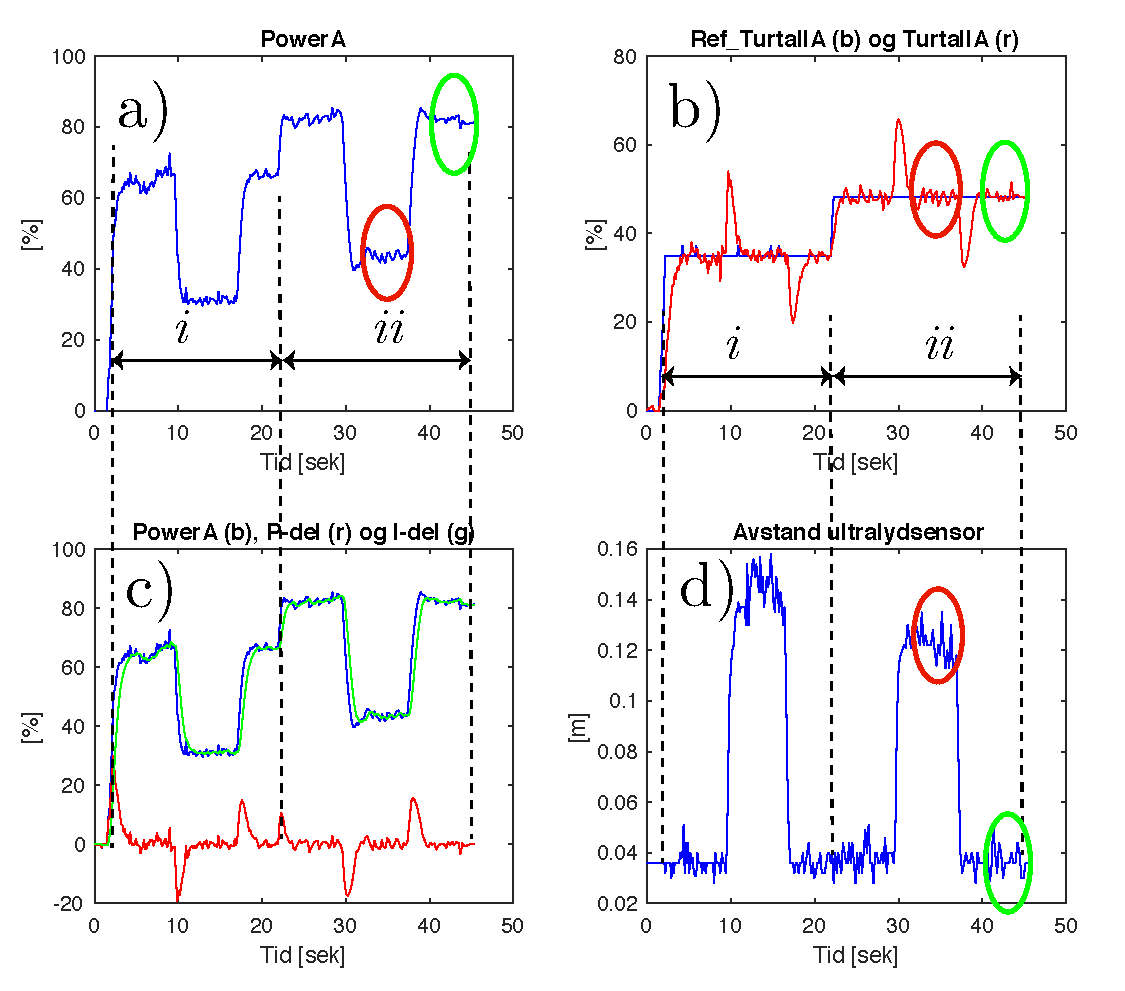
\includegraphics{turtallregulering}}
  \caption{Målinger og beregninger fra et eksperiment som viser
    hvordan turtallregulatoren kompenserer for friksjon. Følgende
    parametre ble benyttet: {\tt alfa1=0.3}, {\tt Kp=1}, {\tt Ki=2},
    {\tt Kd=0}.
    a):~Beregnede pådragsverdier fra PI-regulatoren. 
    b):~Referanse fra potensiometerert (blått) og beregnet
    turtall [\%] (rødt). 
    c):~Bidragene fra P-del (rødt) og I-del (grønt), og totalpådraget {\tt
      PowerA} (blått). 
    d):~Avstandsmålinger fra ultralydsensoren.
    Forklaring
    til resultatene er gitt i teksten.} 
  \label{fig:turtallregulering}
\end{figure}
Når LEGO-konstruksjonen legges ned på bordet,
markert med grønn ring i d),
ser vi fra a) at regulatoren øker pådraget, men at
turtallet etter en kort innsvingningsperiode følger
referansen, markert med grønn ring i b). 


\subsection{Integratorbegrensing}
I dette delkapittel skal vi vise hva som skjer med en standard
PI-regulator når regulatoren ikke klarer å holde utgangen lik
referansen. En slik situasjon kan vi oppnå ved å sette referansen til
100\% for deretter å legge LEGO-konstruksjonen ned på
bordet. Friksjonen vil da bidra til at LEGO-motoren ikke klarer å
holde 100\% turtall, og 
dette er vist i grønn sirkel i figur~\ref{fig:windup}b), hvor
tidsperioden  $23{<}t{<}50$~sekund er delt opp i følgende 
5 delperioder hvor informasjonen lest ut fra delfigurene er listet opp
i en slags kronologisk rekkefølge:

\begin{enumerate}[1.]
\item Gjelder for tidsperioden $23{<}t{<}27$.
  \begin{itemize}
  \item [d)]   LEGO-konstruksjonen er løftet
    opp og motoren er uten  friksjon
  \item [b)] Referansen og utgang er begge 100\% turtall og
    reguleringsavviket er dermed0
    \item [c)] Pådraget er rett i  underkant av 100\%   (markert med \fbox{max}).
  \end{itemize} 
  \todo[noline,size=\footnotesize]{Når figurene inneholder mye data som
  er vanskelig for leseren å intuitivt forstå på egen hånd, er det
  lurt å gi en god og detaljert forklaring på hva resultatene
  viser. Dette viser også at DU har forstått hva som skjer. Dersom du
  ikke gir gode forklaringer på resultater som er vanskelige å forstå,
  vil ikke leseren heller forstå det og det teller negativt inn på
  karakteren. }
\item Gjelder for tidsperioden $27{<}t{<}35$.
  \begin{itemize}
  \item [d)]   LEGO-konstruksjonen hviler på
  bordet og motoren utsettes for friksjon. 
  \item [b)]  Referansen er fortsatt 100\% mens virkelig turtall
    faller til ca. 75\% turtall. Reguleringsavviket er dermed på 25\% (vist med
  loddrett dobbelpil)
  \item [c)] Dette resulterer i at I-leddet integreres lineært.
  \item [a)] Beregnet teoretisk pådrag øker tilsvarende opp til  ca
    500\%, men pådraget er i realiteten ``kun'' 100\%.
  \end{itemize}
\item Gjelder for tidsperioden $35{<}t{<}38$.
  \begin{itemize}
  \item [d)]   LEGO-konstruksjonen er løftet
  opp og motoren er uten
  friksjon.
  \item [b)]   Referansen er fortsatt 100\% mens virkelig turtall
  stiger til ca.  105\% turtall som er det turtallet motoren kan oppnå
  ubelastet ved fullt pådrag (tilsvarer vinkelhastighet på 857 avlest
  i  delfigur c) i figur~\ref{fig:power_vs_turtall}).
  Siden virkelig turtall er noe større enn referansen,
  er reguleringsavviket negativt, altså
  \begin{equation}
    \mathtt{e\_{TurtallA}}\approx -5\%
  \end{equation}
\item [c)]   I denne perioden synker I-leddet fra ca 480 til ca 430
\item [a)]  Totalpådraget synker tilsvarende som I-leddet
\end{itemize}

\begin{figure}[H]
  \centering
  \hspace*{-5mm}\scalebox{0.9}{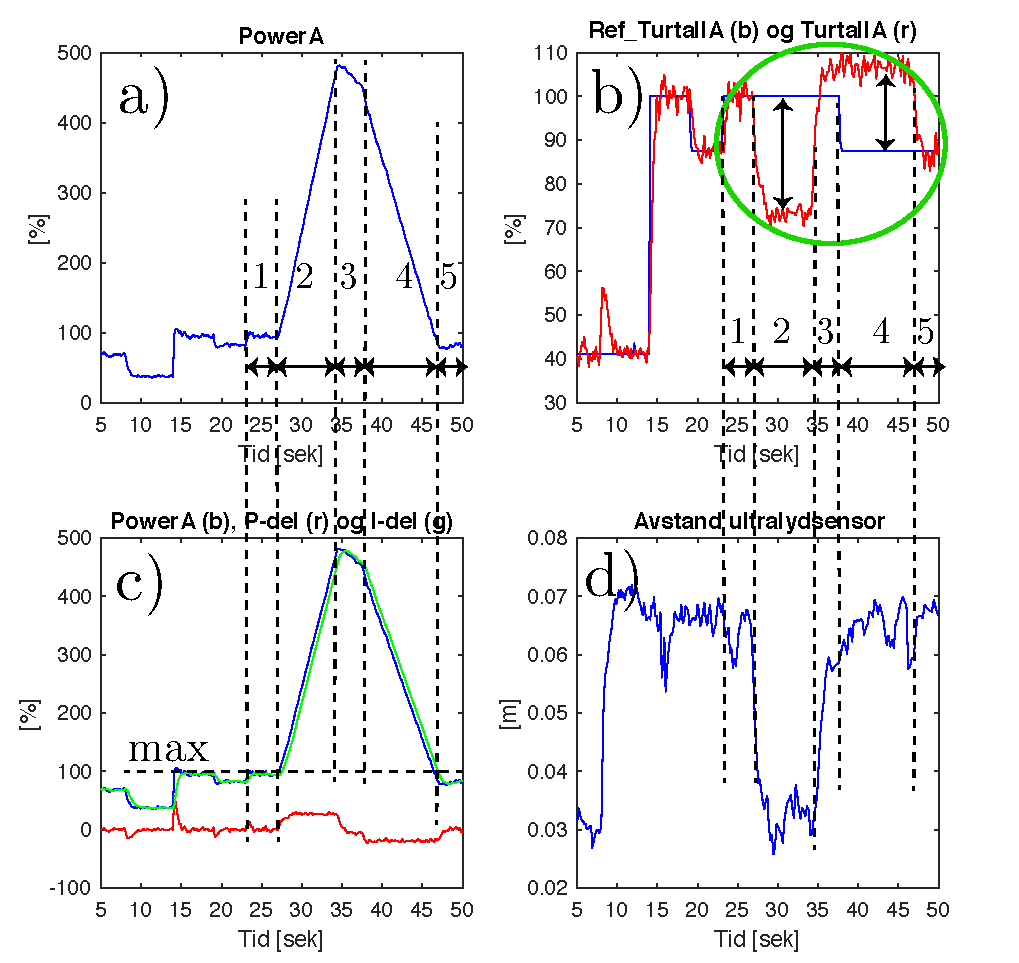
\includegraphics{windup}}
  \caption{Målinger og beregninger fra et eksperiment som viser
    hva som skjer dersom integratoren ikke begrenses når 
    turtallregulatoren ikke klarer å følge referansen. Følgende
    parametre ble benyttet: {\tt alfa1=0.3}, {\tt Kp=1}, {\tt Ki=2},
    {\tt Kd=0}.
    a):~Beregnede pådragsverdier fra PI-regulatoren. 
    b):~Referanse fra potensiometerert (blått) og beregnet
    turtall (rødt). 
    c):~Bidragene fra P-del (rødt) og I-del (grønt), og totalpådraget {\tt
      PowerA} (blått). 
    d):~Avstandsmålinger fra ultralydsensoren.
    Forklaring
    til resultatene er gitt i teksten.}
  \label{fig:windup}
\end{figure}
\newpage
\item Gjelder for tidsperioden $38{<}t{<}47$.
  \begin{itemize}
  \item [d)]   LEGO-konstruksjonen er
  fortsatt løftet opp og motoren er uten
  friksjon.
  \item [b)] Referansen er redusert til ca. 90\% mens virkelig turtall
  fortsatt er  105\% turtall
  Dette gir et større negativt
  reguleringsavvik på 
  \begin{equation}
      \mathtt{e\_{TurtallA}}\approx -15\%
  \end{equation}
  \item [c)] Dette gjør at I-leddet reduseres raskere enn i periode 3. 
    Siden I-leddet fortsatt er større enn max pådrag på 100\% ligger
  turtallet over referansen i hele denne perioden.\footnote{Hadde
    dette vært en {\em cruise controller} til en svært tung bil som i
    en oppoverbakke ikke klarte å holde fartsgrensen, ville bilen
    kjørt mye over fartsgrensen når den passerte toppen av bakken.}
  Legg merke til å P-delen er negativ og den prøver å redusere
  turtallet. 
\end{itemize}
\item Gjelder for tidsperioden $47{<}t{<}50$.
  \begin{itemize}
  \item [d)]   LEGO-konstruksjonen er
  fortsatt løftet opp og motoren er uten
  friksjon
 \item [b)] Referansen er fortsatt ca. 90\%,  men nå er virkelig
   turtall også redusert til  90\% og reguleringsavviket er 0.
 \item [c)]  I-leddet er nå redusert til under 100\%. P-leddet er ca
   0\% siden reguleringsavviket er 0.
 \end{itemize}
\end{enumerate}


Som eksperimentet viser, oppstår problemet i periode 2 hvor
I-leddet integreres etter at pådraget er gått i metning og motoren
ikke lenger klarer å følge referansen. 
Siden integratoren ``må tømmes'' med negativt
reguleringsavvik, vil virkelig turtall
ligge over ønsket turtall i periode 3 og 4, og dette er en uønsket
egenskap.  
Løsningen er å forhindre at I-leddet integreres opp
etter at I-leddet har passert 100\% nivå, og dette løste vi som vist i
kodeutdrag~\ref{kode:antiwindup}.
\begin{lstlisting}[caption=Kode for integratorbegrensing i turtallsregulatoren.,
  label=kode:antiwindup, firstnumber=18]
   I_A(k) = EulerForward(I_A(k-1), Ki*e_TurtallA(k-1), Ts(k-1));
   if abs(I_A(k))>100
       I_A(k)=I_A(k-1);
   end
\end{lstlisting}

Ved å benytte denne koden i et lignende eksperiment som vist i
figur~\ref{fig:windup}, fikk vi resultatene vist 
i figur~\ref{fig:PI_anti_reg} hvor de 
grønne ringene i markerer effekten av integratorbegrensingen. I
delfigur d) blir 
LEGO-konstruksjonen blir lagt ned på bordet i tidsperioden $17<t<24$.
Samtidig faller turtallet i b) på samme måte som i periode~2 i
figur~\ref{fig:windup} hvorpå det blir et vedvarende reguleringsavvik
større enn 0,
men integratorbegrensingen gjør at I-leddet stopper på 100\% i
c). Når LEGO-konstruksjonen løftes opp fra bordet ved $t>24$, går
turtallet opp til referansen med en gang, og
reguleringsavviket er 0. 
\begin{figure}[H]
  \centering
  \hspace*{-5mm}\scalebox{0.8}{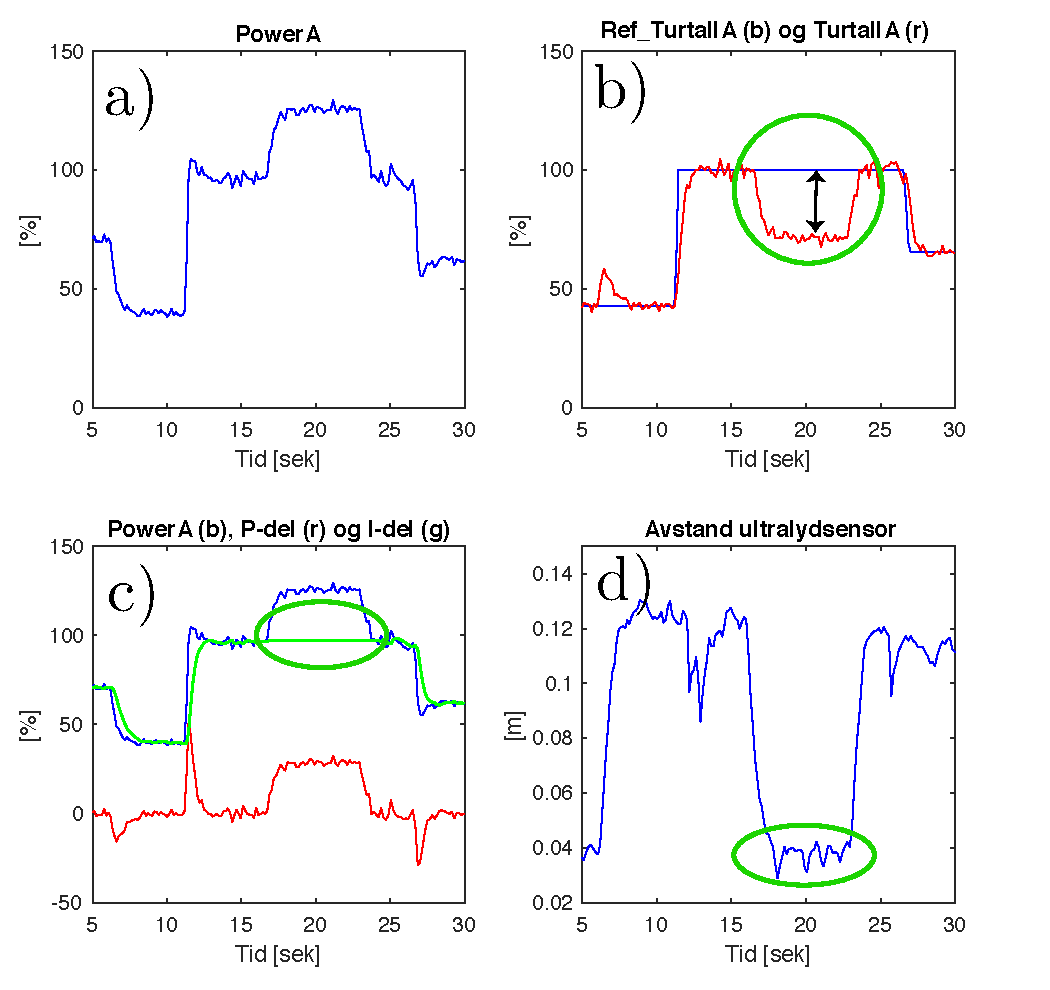
\includegraphics{PI_anti_reg}}
  \caption{Målinger og beregninger fra et eksperiment som viser
    effekten av integratorbegrensing.  Følgende
    parametre ble benyttet: {\tt alfa1=0.3}, {\tt Kp=1}, {\tt Ki=2},
    {\tt Kd=0}.
    a):~Beregnede pådragsverdier fra PI-regulatoren. 
    b):~Referanse fra potensiometerert (blått) og beregnet
    turtall (rødt). 
    c):~Bidragene fra P-del (rødt) og I-del (grønt), og totalpådraget {\tt
      PowerA} (blått). 
    d):~Avstandsmålinger fra ultralydsensoren.
    Forklaring
    til resultatene er gitt i teksten.} 
  \label{fig:PI_anti_reg}
\end{figure}

\subsection{PID-regulator}
Ved å legge til D-delen av PID-regulatoren, vil totalpådraget få et
bidrag som er bestemt ut fra hvor fort reguleringsavviket
{\em endres}. 
Resultatet fra et forsøk med en PID-regulator er vist i
figur~\ref{fig:PID_reg}, hvor den største
effekten av D-delen er markert med
grønne og røde ringer.

\begin{figure}[H]
  \centering
  \hspace*{0mm}\scalebox{0.71}{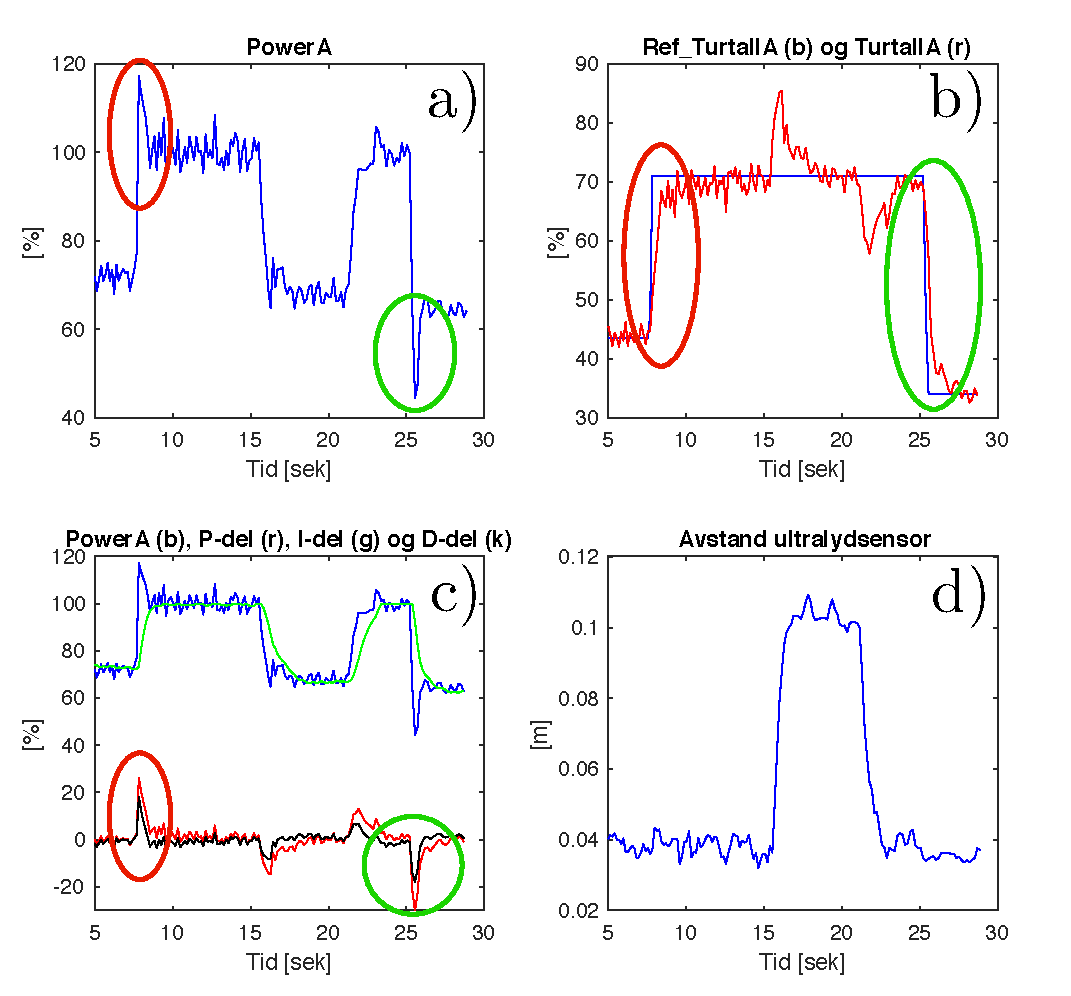
\includegraphics{PID_reg}}
  \caption{Målinger og beregninger fra et eksperiment som viser
    hvordan PID-versjonen av turtallregulatoren kompenserer for friksjon. Følgende
    parametre ble benyttet: {\tt alfa1=0.3}, {\tt Kp=1}, {\tt Ki=2},
    {\tt Kd=1}, {\tt alfa2=0.1}.
    a):~Beregnede pådragsverdier fra PID-regulatoren. 
    b):~Referanse fra potensiometerert (blått) og beregnet
    turtall (rødt). 
    c):~Bidragene fra P-del (rødt), I-del (grønt), D-del (svart) 
    og totalpådraget {\tt
      PowerA} (blått). 
    d):~Avstandsmålinger fra ultralydsensoren.
    Forklaring
    til resultatene er gitt i teksten.} 
  \label{fig:PID_reg}
\end{figure}
Følgende regulatorparametre er benyttet; 
{\tt Kp=1}, {\tt Ki=2},   {\tt Kd=1}. I filteret som benyttes i
derivatdelen benyttet vi {\tt alfa2=0.1}.

Siden bidraget fra D-delen gjør seg gjeldene når reguleringsavviket
endres, ser vi at den positive referanseendringen ved $t=7$ sekund
(rød ring, delfigur b)) bidrar til at D-delen gir en positivt, men kortvarig
bidrag (delfigur c)). Dette gjør at turtallet stiger raskere enn det
ville gjort uten D-delen. Legg merke til at i a) så går totalpådraget
over 100\% som betyr at regulatoren egentlig ikke får fullt utnyttet 
effekten av D-delen.

Derimot så viser responsen markert med grønne ringer et eksempel på
at regulatoren får fullt utbytte av D-delen. Den negative
referanseendringen gjør at D-delen bidrar med negative verdier (vist i
c)), og at totalpådraget i a) går helt ned mot 40\% pådrag før den
stabiliserer seg på 65\% mot slutten. Effekten på turtallet er at det
faller raskere enn uten D-del.


En siste viktig, men negativ, bi-effekt av D-delen er at 
pådraget blir mer støyfylt når reguleringsavviket
deriveres. Dette kan reduseres ved å filtrere enda kraftigere (lavere verdi
på {\tt alfa2}). 







\subsection{Effekten av å kople inn turtallsregulatoren}\label{kap:auto_manuell}


For å få vist effekten av å kople inn og ut turtallsregulatoren under kjøring, bestemte
vi oss for å benytte potensiometeret 
både som direkte pådrag (i ``manuell'') og som 
referanse (i ``auto''). 
Dette er vist i 
kodeutdrag~\ref{kode:turtall} hvor vi bestemmer funksjonen til
turtallsregulatoren ved å trykke på en LEGO-trykkbryter. Er den
inntrykket er regulatoren i manuell og
pådraget til motoren settes til  potensiometerverdien. Dette er vist i
linje 16 i koden under. 

For å unngå problemer i plottingen av dataene ved at det mangler
verdier i vektorene, setter vi {\tt P\_A(k)=NaN} og {\tt D\_A(k)=NaN}.
I tillegg justerer vi kontinuerlig integratorleddets verdi som vist i
linje 18. Dermed unngår vi at I-leddet integrerer seg opp eller ned mens vi kjører i
manuell, og  i det vi kopler over til automatisk kjøring, vil regulatoren
starte med samme pådrag som den hadde i manuell. Dette gir en såkalt
støtfri omkopling, eller {\it bumpless transfer}. 
\newpage
\begin{lstlisting}[caption=Kode for turtallsregulator for motor A.,
  label=kode:turtall, firstnumber=11]
% trykknapp bestemmer om regulator er i auto eller manuel
TurtallsReg(k) = ~Bryter(k);
if TurtallsReg(k)
   PowerA(k) = P_A(k)+I_A(k) + D_A(k);
else
   PowerA(k) = PotMeter(k);
   P_A(k) = NaN;
   I_A(k) = PowerA(k);
   D_A(k) = NaN;
end
motorA.Speed = PowerA(k);
start(motorA);   
\end{lstlisting}

Resultatet av  eksperimentet er vist i
figur~\ref{fig:auto_man}, hvor LEGO-konstruksjonen har hvilt på bordet
under hele eksperimentet (delfigur d)). Regulatoren er koplet ut
i tidsperiodene merket
med $i$ og $ii$. Vi observerer at turtallet faller i disse
tidsperiodene, markert med grønne ringer i delfigur b).


\begin{figure}[H]
  \centering
  \hspace*{0mm}\scalebox{0.71}{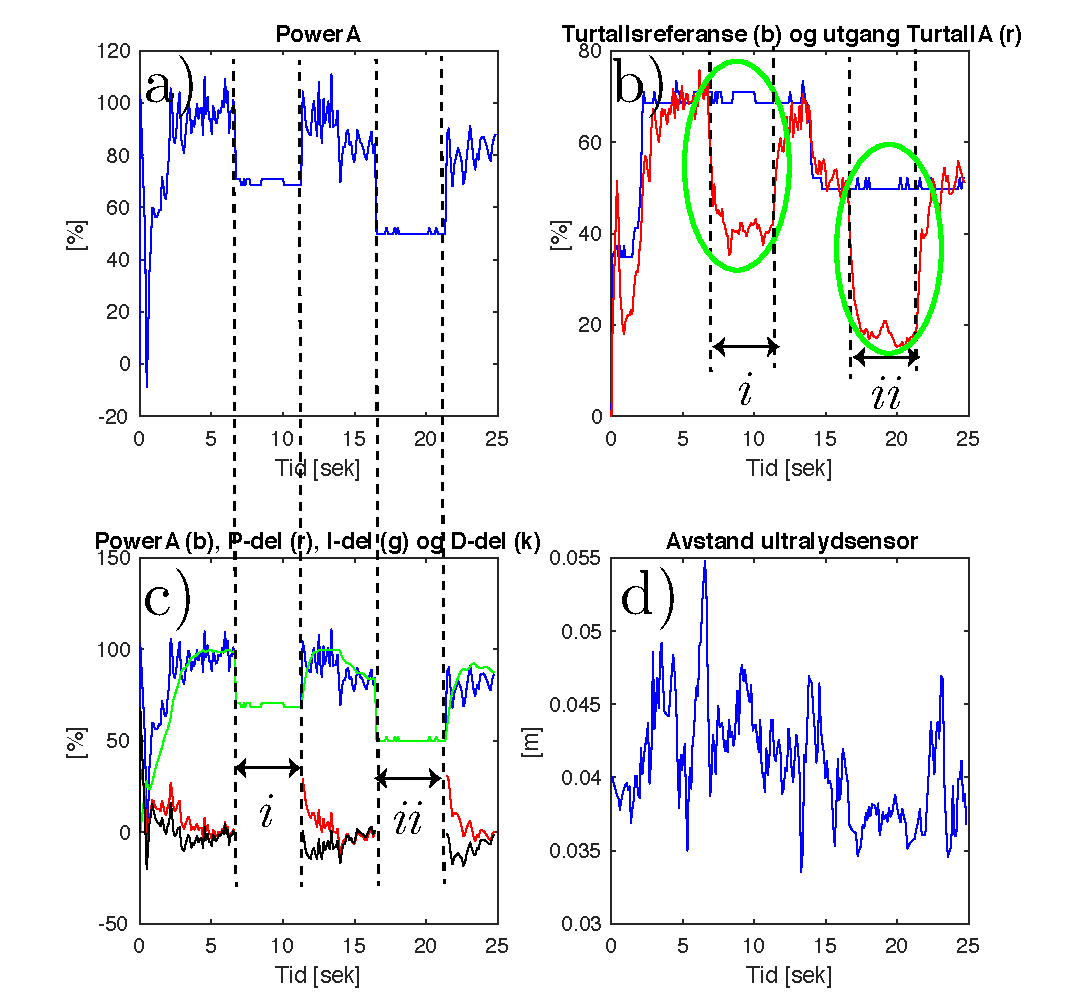
\includegraphics{auto_man}}
  \caption{Målinger og beregninger fra et eksperiment som viser
    effekten av å kople inn og ut
    turtallsregulatoren. Turtallsregulatoren er utkoplet i
    tidsperiodene merket med $i$ og $ii$. Følgende
    parametre ble benyttet: {\tt alfa1=0.3}, {\tt Kp=1}, {\tt Ki=2},
    {\tt Kd=1}, {\tt alfa2=0.1}.
    a):~Beregnede pådragsverdier fra PID-regulatoren, samt manuelt
    pådrag i periodene $i$ og $ii$. 
    b):~Referanse fra potensiometerert (blått) og beregnet
    turtall (rødt). 
    c):~Bidragene fra P-del (rødt), I-del (grønt), D-del (svart) 
    og totalpådraget {\tt
      PowerA} (blått). Legg merke til at P-del og I-del er NaN i
    perioden med manuelt pådrag. I-delen beholdes som manuelt pådrag
    for å unngå store endringer ved innkopling. 
    d):~Avstandsmålinger fra ultralydsensoren viser at LEGO-konstruksjonen har
    ligget på bordet under hele forsøket.} 
  \label{fig:auto_man}
\end{figure}

\newpage

\section{Turtallsregulator som funksjon}\label{kap:funksjon}
For å kunne bruke turtallsregulatorkoden på en enkel måte i
prosjektene våre, laget vi en funksjon av koden. Vi har brukt
  \todo[size=\footnotesize]{Bruk av {\it persistent} vil bli gått
    gjennom i undervisningen. }
{\it  peristent}-funksjonaliteten i MATLAB, og kan på den måten spare
endel oversending av data i funksjonskallet.

Siden variable som blir definert som {\it persistent} vil ligge
tilgjengelig lokalt i funksjonen til neste gang den blir kallet, vil
det ikke fungere å bruke samme funksjon til å beregne pådrag for flere
motorer. Dette fordi tallverdiene for de forskjellige motorene vil bli
blandet. Av den grunn har vi laget tre identiske funksjoner kalt
\fbox{\tt CalcPowerA.m}, \fbox{\tt CalcPowerB.m} 
og \fbox{\tt CalcPowerC.m}.

Under blir koden til \fbox{\tt CalcPowerA.m} vist.
I selve funksjonskallet sendes
\begin{itemize}
\item motorobjektet, for avlesing av vinkelposisjon inne i selve
  funksjonen
\item referansen, som tilsvarer enten ønsket turtall eller manuelt pådrag 
\item regulatorfunksjonalitet, som P, PI, PD, I, PID eller manuell.
\item regulatorparametre
\end{itemize}

Deretter spesifiseres de variable som er lokale for funksjonen, og
standardverdier for regulatorparametre, se kodeutdrag~\ref{kode:turtall_mA}.

\begin{lstlisting}[caption=Kode fra funksjonen for turtallsregulering av motor A.,
  label=kode:turtall_mA, firstnumber=18]
function [u,varargout] = CalcPowerA(motorA,SpeedRef,action,varargin)

persistent e e_IIR angle angle_IIR timestamp I 

% default values of parameters
Kp    = 1;
Ki    = 2;
Kd    = 1;
umax  = 100;
umin  = -100;
alfa1 = 0.3; % angular velocity filtering
alfa2 = 0.1; % error filtering in D-part
\end{lstlisting}

Dersom brukeren ønsker å sende inn andre regulatorparametre, kan dette
sendes inn som \fbox{varargin} som inneholder en {\tt struct} med
parameterverdier. For å overskrive standardverdiene vist over, brukes
følgende kode:
\begin{lstlisting}[caption=Kode fra funksjonen for turtallsregulering av motor A.,
  label=kode:para, firstnumber=31]
  % If you have specified some parameters in main file, they will overwrite
% the default values in this function
if nargin>3
    paranew=varargin{1};     
    if isfield(paranew,'Kp')
        Kp = paranew.Kp;
    elseif isfield(paranew,'Ki')
        Ki = paranew.Ki;
    elseif isfield(paranew,'Kd')
        Kd = paranew.Kd; 
    elseif isfield(paranew,'umax')
        umax = paranew.umax; 
    elseif isfield(paranew,'umin')
        umin = paranew.umin; 
    elseif isfield(paranew,'alfa1')
        alfa1 = paranew.alfa1; 
    elseif isfield(paranew,'alfa2')
        alfa2 = paranew.alfa2; 
    end
end
\end{lstlisting}

Ved bruk av {\it persistent} variable, trenger vi ikke ta vare på
mer enn de  2 siste
elementene i variablene. Ved å spesifisere element nr 2 i disse
variablene til 0 som vist i kodeutdraget under,
blir også element nr 1 satt lik 0 dersom den ikke
allerede har et innhold.

Ved aller første gangs kall av funksjonen har
ikke element nr 1 innhold, men ved å flytte element nr 2 til element
nr 1 i slutten av funksjonen (samme som å gå ett tidsskritt frem),
vil element nr 1 ha innhold ved neste
kall, og element nr 1 blir derfor ikke overskrevet til 0.

\begin{lstlisting}[caption=Kode fra funksjonen for turtallsregulering av motor A.,
  label=kode:resten, firstnumber=31]
angle(2)=0;
angle_IIR(2)=0;
e(2)=0;
e_IIR(2)=0;
I(2)=0;
\end{lstlisting}

Resten av koden tilsvarer det som er vist  i
kodeutdragene~\ref{kode:vinkelHast}, \ref{kode:rotHast},
\ref{kode:e_RHA}, \ref{kode:P_del}, \ref{kode:I_del},
\ref{kode:D_del} og \ref{kode:PID}, og er vist i sin helhet under.
\begin{lstlisting}[caption=Kode fra funksjonen for turtallsregulering av motor A.,
  label=kode:resten2, firstnumber=31]
timestamp(2) = toc;
Ts = timestamp(2)-timestamp(1); 
angle(2)     = double(motorA.readRotation);
angle_IIR(2) = IIR_filter(angle_IIR(1),angle(2),alfa1);
angular_speed = Derivation(angle_IIR, Ts);
speed = 1/8*angular_speed;
e(2) = SpeedRef - speed;
P = Kp*e(2);
I(2) = EulerForward(I(1), Ki*e(1), Ts);
if I(2)>umax
    I(2)=I(1);
elseif I(2)<umin
    I(2)=I(1);
end
e_IIR(2) = IIR_filter(e_IIR(1), e(1), alfa2);
D = Derivation(Kd*e_IIR, Ts);
\end{lstlisting}

Ut fra regulatorfunksjon, bestemmes deretter hvilket pådrag som skal
beregnes. Valgene er P-regulator, PI, PID, PD, I eller manuell, se
under.
  \todo[noline,size=\footnotesize]{Siden innholdet i dette
    delkapittelet blir veldig mye kode og lite beskrivende tekst,
    merker du kanskje selv at du ikke bruker tid
    på å lese denne delen. Det beste ville vært å ha en liten
    introduksjon til tankegangen bak funksjonen, og legge hele
    koden i et vedlegg. Dersom du opplever at deler av din egen
    rapport ligner på akkurat denne siden her, vil leseren mest sannsynlig
    bare hoppe over dette (sensor også).

    Jeg har gjort dette med vilje her bare for at du skal se hvordan
    rapporten IKKE skal se ut. }
\begin{lstlisting}[caption=Kode fra funksjonen for turtallsregulering av motor A.,
  label=kode:resten3, firstnumber=31]
if strcmp(action,'P') 
    u = P;
    I(2)=NaN;
    D=NaN;
elseif strcmp(action,'PI')
    u = P + I(2);
    D=NaN;
elseif strcmp(action,'PID')
    u = P + I(2) + D;
elseif strcmp(action,'PD')
    u = P + D;
    I(2)=NaN;
elseif strcmp(action,'I')
    u = I(2);
    P=NaN;
    D=NaN;
elseif strcmp(action,'man')
    u = SpeedRef;
    I(2)=SpeedRef;
    P=NaN;
    D=NaN;
end
\end{lstlisting}

Til slutt flyttes dataene i element 2 til element 1, som innebærer det
samme som å gå et tidsskritt frem. Samtidig gjøres variablene i
\fbox{\tt varargout} klar, se  under.
\begin{lstlisting}[caption=Kode fra funksjonen for turtallsregulering av motor A.,
  label=kode:resten4, firstnumber=31]
angle(1)     = angle(2);
angle_IIR(1) = angle_IIR(2);
e(1)         = e(2);
e_IIR(1)     = e_IIR(2);
timestamp(1) = timestamp(2);
I(1)         = I(2);

outputarg = [P,I(2),D];
nout = max(nargout,1) - 1;
for k = 1:nout
   varargout{k} = outputarg(k);
end


\end{lstlisting}







\chapter{Litt om referering til rapportelementer}\label{kap:referering}

\section{{\em Tagging} av rapportelement, \fbox{\tt $\backslash$label\{ \}}}\label{delkap:label}
For at du i teksten du skriver 
skal kunne referere til forskjellige rapportelementer må du legge til en
{\em tag} eller {\em bookmark} som tydelige identifiserer selve
elementet. Til dette bruker du kommandoen 
\fbox{\tt $\backslash$label\{ \} }, hvor det som står inne i
krøllparentesene er den unike referanseteksten/identifikasjonen for elementet.
Siden det finnes veldig mange forskjellige rapportelementer som det kan
refereres til, er det vanlig å bygge opp selve referanseteksten slik:\\[-10mm]
\begin{center}
  {\tt $\backslash$label\{forkortelse for elementet:\underline{beskrivende tekst}\}}
\end{center}
\vspace*{-5mm}
Eksempler på typiske rapportelementer og forkortelser  er
vist i listen under, hvor {\tt xxxxx} er satt inn for \underline{\tt
  beskrivende tekst}.
\vspace*{-3mm}
\begin{enumerate}
\item For å referere til {\color{red}kapitler} benyttes ofte \fbox{\tt kap} som
  forkortelse\footnote{Dersom du vil bruke engelske ord er \fbox{\tt
      ch}  for {\tt $\backslash$chapter} et godt alternativ.}, og  
  {\tt $\backslash$label\{kap:xxxxx\}} må plasserers innenfor selve
  kapittelet, og typisk rett bak 
  {\tt $\backslash$chapter\{Kapitteloverskrift\}}. Helt øverst i selve .tex-fila til dette
  kapittelet, \fbox{\tt litt\_om\_referering.tex}, vil du se måten det
  er gjort på her:\\
 {\tt $\backslash$chapter\{Litt om referering til 
    rapportelementer\}$\backslash$label\{kap:referering\} } 

\item For å referere til {\color{red}delkapitler} benyttes ofte \fbox{\tt delkap} som
  forkortelse\footnote{Dersom du vil bruke engelske ord er \fbox{\tt
      sec} for {\tt $\backslash$section} et godt alternativ.}, og ellers gjøres det på samme måte som for
  kapitler. For dette delkapittelet (kapittel~\ref{delkap:label}) er
  følgende {\em tag} brukt   {\tt $\backslash$label\{delkap:label\}}.

\item For å referere til {\color{red}ligninger} benyttes ofte \fbox{\tt eq} som
  forkortelse, og {\tt $\backslash$label\{eq:xxxxx\}}  plasseres
  mellom {\tt $\backslash$begin\{equation\}} og 
  {\tt $\backslash$end\{equation\}} som vist   under

  \begin{boxedminipage}{\textwidth}
\begin{verbatim}
\begin{equation}
  \label{eq:sinus}             <-----------------
  y(t)=\sin(\omega t)
\end{equation}
\end{verbatim}
  \end{boxedminipage}

  Dette blir vist mer i detalj i kapittel~\ref{kap:ligninger}. \label{pkt:ligning}

\item For å referere til {\color{red}figurer} benyttes ofte \fbox{\tt fig} som
  forkortelse, og  {\tt $\backslash$label\{fig:xxxxx\}} plasseres
  mellom {\tt $\backslash$begin\{figure\}} og 
  {\tt $\backslash$end\{figure\}} som vist under

  \begin{boxedminipage}{\textwidth}
\begin{verbatim}
\begin{figure}[H]
  \centering
  \scalebox{0.6}{\includegraphics{sinuskurve}}
  \caption{Figuren viser en sinuskurve som funksjon av tid.} 
  \label{fig:sinuskurve}             <-----------------
\end{figure}
\end{verbatim}
  \end{boxedminipage}

Dette blir vist mer i detalj i kapittel~\ref{kap:figurer}. 

\item For å referere til {\color{red}tabeller} benyttes ofte \fbox{\tt tab} som
  forkortelse, og {\tt $\backslash$label\{tab:xxxxx\}} plasseres
  mellom {\tt $\backslash$begin\{table\}} og 
  {\tt $\backslash$end\{table\}} som vist under

  \begin{boxedminipage}{\textwidth}
\begin{verbatim}
\begin{table}[H]
  \centering
  \caption{Enkel tabell.}
  \begin{tabular}{|c|c|}\hline
    a & b   \\\hline\hline 
    2 & 0.6 \\\hline
  \end{tabular}
  \label{tab:a_og_b}             <-----------------
\end{table}
\end{verbatim}
  \end{boxedminipage}

Dette blir vist mer i detalj i kapittel~\ref{kap:tabeller}.

\item For å referere til {\color{red}\fbox{\tt
      $\backslash$item}-elementer} i en punktliste  benyttes ofte
  \fbox{\tt pkt} som  forkortelse, og {\tt $\backslash$label\{pkt:xxxxx\}}
  plasseres bak teksten som tilhører punktet. 
  Du kan IKKE bruke dette i {\tt $\backslash$begin\{itemize\}} og 
  {\tt $\backslash$end\{itemize\}} siden punktene er svarte, unummererte
  prikker. Du kan kun referere i lister laget av {\tt $\backslash$begin\{enumerate\}} og 
  {\tt $\backslash$end\{enumerate\}} som vist i eksempelet under

  \begin{boxedminipage}{\textwidth}
\begin{verbatim}
\begin{enumerate}
\item Biler er gule.
\item Roser er røde. \label{pkt:roser}             <-----------------
\end{enumerate}
\end{verbatim}
  \end{boxedminipage}

Dette blir vist mer i detalj i kapittel~\ref{kap:punktlister}.

\item For å referere til {\color{red}sidenummer} benyttes ofte
  \fbox{\tt side} som  forkortelse, og 
  {\tt  $\backslash$label\{side:xxxxx\}} plasserer
  rett i teksten og nær teksten du ønsker å referere til. \label{pkt:side}
\end{enumerate}
Legg merke til at den \underline{beskrivende teksten} kan være hva som helst, og
gjerne identisk med andre beskrivende tekster. Sammenkoplingen av
forkortelser av elementer og beskrivende tekst gjør alikevel selve
referansen helt unik.
{\color{red}Husk at du aldri må bruke  æ,ø eller å i referansetekstene.}

\section{{\em Tagging} av kode, \fbox{\tt label= }}
Dersom du bruker  \fbox{\tt listings}-pakken slik
det blir beskrevet i
kapittel~\ref{kap:kode}, brukes \fbox{\tt label} på en litt annen måte. 
Istedenfor å skrive \fbox{\tt $\backslash$label\{kode:xxxxx\}} skal du heller skrive
\fbox{\tt label=kode:xxxxx}. Denne skal plasseres i hakeparentes
sammen med {\tt caption} og eventuelle linjenummerspesifikasjoner som vist i
følgende eksempel:

\begin{boxedminipage}{\textwidth}
\begin{verbatim}
\lstinputlisting[firstnumber=14,firstline=14,lastline=28,
          caption={Utdrag av funksjonen {\tt SaveMyFigure.m}.},
            label=kode:Utdrag_av_SaveMyFigure]{SaveMyFigure.m}
\end{verbatim}
\end{boxedminipage}

Dette eksempelet viser kodelinjene 14-28 fra filen 
\fbox{\tt SaveMyFigure.m} som ligger i samme mappe som hovedfilen 
{\tt  Gruppe19XX.tex}.
Resultatet av denne koden er vist i kodeutdrag~\ref{kode:Utdrag_av_SaveMyFigure} 
    på side~\pageref{kode:Utdrag_av_SaveMyFigure}.

Dette blir vist mer i detalj i kapittel~\ref{kap:kode}.

\section{Bruk av \fbox{\tt $\backslash$ref\{ \}}, \fbox{\tt
    $\backslash$eqref\{ \}} og \fbox{\tt $\backslash$pageref\{ \}}}\label{delkap:ref}
For å referere til  kapitler, ligninger, figurer, tabeller og punktlister 
brukes \fbox{\tt $\backslash$ref\{ \}}. 
For å referere til {\em ligninger} bør du bruke
\fbox{\tt $\backslash$eqref\{ \}} som sørger for at parentesene som
omslutter ligningsnummeret blir med i teksten.
For å referere til {\em sidenummer} 
må du bruke  \fbox{\tt $\backslash$pageref\{ \}}.

Under er vist et overdrevent eksempel på referering til en ligning gitt på en side
i et kapittel (vanligvis holder det å referere kun til
ligningsnummeret).

\begin{boxedminipage}{\textwidth}
\begin{verbatim}
Som vist i ligning~\eqref{eq:IIR-filter} på side~\pageref{side:integrasjon},  
gitt i kapittel~\ref{kap:integrasjon}, benyttes et IIR-filter for å
beregne filtrert lys. 
\end{verbatim}
\end{boxedminipage}

Bruken av tilde mellom ordet \fbox{\tt ligning} og koden \fbox{\tt
  $\backslash$eqref\{eq:IIR-filter\}} er for å knytte disse to elementene
sammen slik at de ikke kan deles/separeres. På den måten unngår du at
ny linje begynner med et ligningsnummer (som kan forveksles med en
slags nummerert liste).

\newpage
\section{Beskrivelse av litteratur}
For å kunne referere til litteratur, må du først lage en .bib-fil som du f.eks. kan
kalle \fbox{\tt referanser.bib} I denne filen ligger data om all
litteratur du bruker, og dataene organiseres i en spesiell struktur som 
typisk ser slik ut:

\begin{boxedminipage}{\textwidth}
\begin{verbatim}
@TypeLitteratur{Tag,
  author =  {},
  title  =  {},
  year   =  {},
  +
  +
}
\end{verbatim}
\end{boxedminipage}

hvor 
\begin{itemize}
\item  \fbox{\tt @TypeLitteratur} kan være bl.a. {\tt @Book}, 
  {\tt @TechReport}, {\tt @Misc}, {\tt @Article}, {\tt @InProceedings}, {\tt Article}, 
  {\tt @PhDThesis},  {\tt @MastersThesis} og {\tt @Unpublished}\footnote{Det
  finnes mange flere varianter.}. Disse blir
  beskrevet i mer detalj nedenfor, men det 
  er \fbox{\tt @Book}, 
  \fbox{\tt @TechReport} og \fbox{\tt @Misc} som er mest relevant for deg 
  i ING100, mens de
  andre typene er mer aktuelle å bruke i bacheloroppgaven din.
  
\item \fbox{\tt Tag} er en {\em tag} på samme måte som andre
  rapportelementer beskrives med en unik nøkkel. Det er mange måter å
  bygge en slik {\em tag} opp på, men en relativt vanlig variant er at
  ta de 3 første bokstavene i etternavnet til hver forfatter og til
  slutt årstallet. Dersom det er mange forfatttere kan {\em tag}'en
  bli veldig lang, og da pleier jeg å ta med 3 bokstaver fra
  etternavnet til første forfatter og deretter skrive {\tt \_et\_al.}
  som er latisk forkortelse for ``med flere''.  
\item {\tt author}, {\tt title}, {\tt year} og andre elementer
  varierer med hvilken type publikasjon vi snakker om. Dette blir vist
  mer i detalj nedenfor
\end{itemize}


Et eksempel på en .bib-fil ligger i
samme mappe som hovedfilen {\tt Gruppe19XX.tex}.
Den heter {\tt referanser.bib} og inneholder ett eksemlar av typene
{\tt @Book},   {\tt @TechReport} og {\tt @Misc}, og disse blir beskrevet
i den neste 3 delkapitlene.


\subsection{\fbox{\tt @Book}}
{\tt @Book}  bruker du når du skal referere til noe i en bok,
f.eks. læreboka i MAT100~\cite{AdaEss2017}. I {\tt referanser.bib} ser den slik ut:


\begin{boxedminipage}{\textwidth}
\begin{verbatim}
@Book{AdaEss2017,
  author = 	 {R. A. Adams and C. Essex},
  title = 	 {Calculus. A complete course},
  publisher = 	 {Pearson},
  year = 	 {2017},
  edition = 	 {9},
}
\end{verbatim}
\end{boxedminipage}

Legg merke til at hver forfatter skilles med ordet {\em and}.

Den fullstendige beskrivelsen av \fbox{\tt @Book} er

\begin{verbatim}
@Book{,
  ALTauthor = 	 {},
  ALTeditor = 	 {},
  title = 	 {},
  publisher = 	 {},
  year = 	 {},
  OPTkey = 	 {},
  OPTvolume = 	 {},
  OPTnumber = 	 {},
  OPTseries = 	 {},
  OPTaddress = 	 {},
  OPTedition = 	 {},
  OPTmonth = 	 {},
  OPTnote = 	 {},
  OPTannote = 	 {}
}
\end{verbatim}
hvor elementene \fbox{\tt ALTauthor}  og \fbox{\tt ALTeditor} betyr at du må
velge ett 
av alternativene og samtidig fjerne ordet \fbox{\tt ALT}. Ordet
\fbox{\tt OPT} som står foran de nederste elementene betyr {\em
  optional} og trenger ikke fylles ut. De eneste feltene som er
obligatoriske er {\tt author}/{\tt editor}, {\tt title}, {\tt publisher} og {\tt year}.


\subsection{\fbox{\tt @TechReport}}
{\tt @TechReport} brukes for tekniske rapporter som verken er
lærebøker eller artikler. Prosjektbeskrivelsen i ING100 kan kalles en
teknisk rapport, og den referansen ser slik ut i {\tt referanser.bib}.

\begin{boxedminipage}{200mm}
\begin{verbatim}
@TechReport{Dre2019,
  author = 	 {T. Drengstig},
  title = 	 {Lego Mindstorms og MATLAB; anvendt matematikk og fysikk i skjønn forening},
  institution =  {Universitet i Stavanger},
  year = 	 {2019},
  note = 	 {Utdelt materiale},
}
\end{verbatim}
\end{boxedminipage}

Den fullstendige beskrivelsen av \fbox{\tt @TechReport} er
\begin{verbatim}
@TechReport{,
  author = 	 {},
  title = 	 {},
  institution =  {},
  year = 	 {},
  OPTkey = 	 {},
  OPTtype = 	 {},
  OPTnumber = 	 {},
  OPTaddress = 	 {},
  OPTmonth = 	 {},
  OPTnote = 	 {},
  OPTannote = 	 {}
}
\end{verbatim}
Ordet \fbox{\tt OPT} som står foran de nederste elementene betyr {\em
  optional} og trenger ikke fylles ut. De eneste feltene som er
obligatoriske er {\tt author}, {\tt title}, {\tt institution} og {\tt year}.

\newpage

\subsection{\fbox{\tt @Misc}}
{\tt @Misc} brukes for diverse ting, derfor typen {\em
  miscellaneous}. Den fullstendige beskrivelse er gitt under, hvor
alle elementene er {\em optional}. 

\begin{verbatim}
@Misc{,
  OPTkey = 	 {},
  OPTauthor = 	 {},
  OPTtitle = 	 {},
  OPThowpublished = {},
  OPTmonth = 	 {},
  OPTyear = 	 {},
  OPTnote = 	 {},
  OPTannote = 	 {}
}
\end{verbatim}

Denne kan være nyttig til å referere til nettsteder slik som vist på
dette nettstedet~\cite{web_BibTex}, hvor selve referansen ser slik ut i
{\tt referanser.bib}:

\begin{boxedminipage}{200mm}
\begin{verbatim}
@Misc{web_BibTex,
  title = 	 {How can {I} use Bibtex to cite a web page?},
  howpublished = {https://tex.stackexchange.com/questions/3587/how-can-i-use-bibtex-to-cite-a-web-page},
}
\end{verbatim}
\end{boxedminipage}


Legg merke til at for at ``I'' skal forbli en stor i tittelen når den
gjengis i referanselista, må du 
bruke krøllparenteser rundt (som vist med {\tt \{I\}}. 


\newpage

\subsection{\fbox{\tt @Article}}
{\tt @Article} er en artikkel som er publisert i en journal
. Et eksempel er denne
  {\color{red}\href{https://bit.ly/2SCNDdq}{https://bit.ly/2SCNDdq}}
  som er en såkalt oversiktsartikkel ({\em review}-artikkel) 
  om bruken av  LEGO i høyere
  utdanning de siste 15 år. Den er publisert i International Journal
  of Advanced Robotic Systems.
Ved å trykke på
  {\color{red}{Download PDF}}-knappen vil du se at artikkelen ser
  slik ut.
\begin{figure}[H]
  \centering
  \scalebox{0.5}{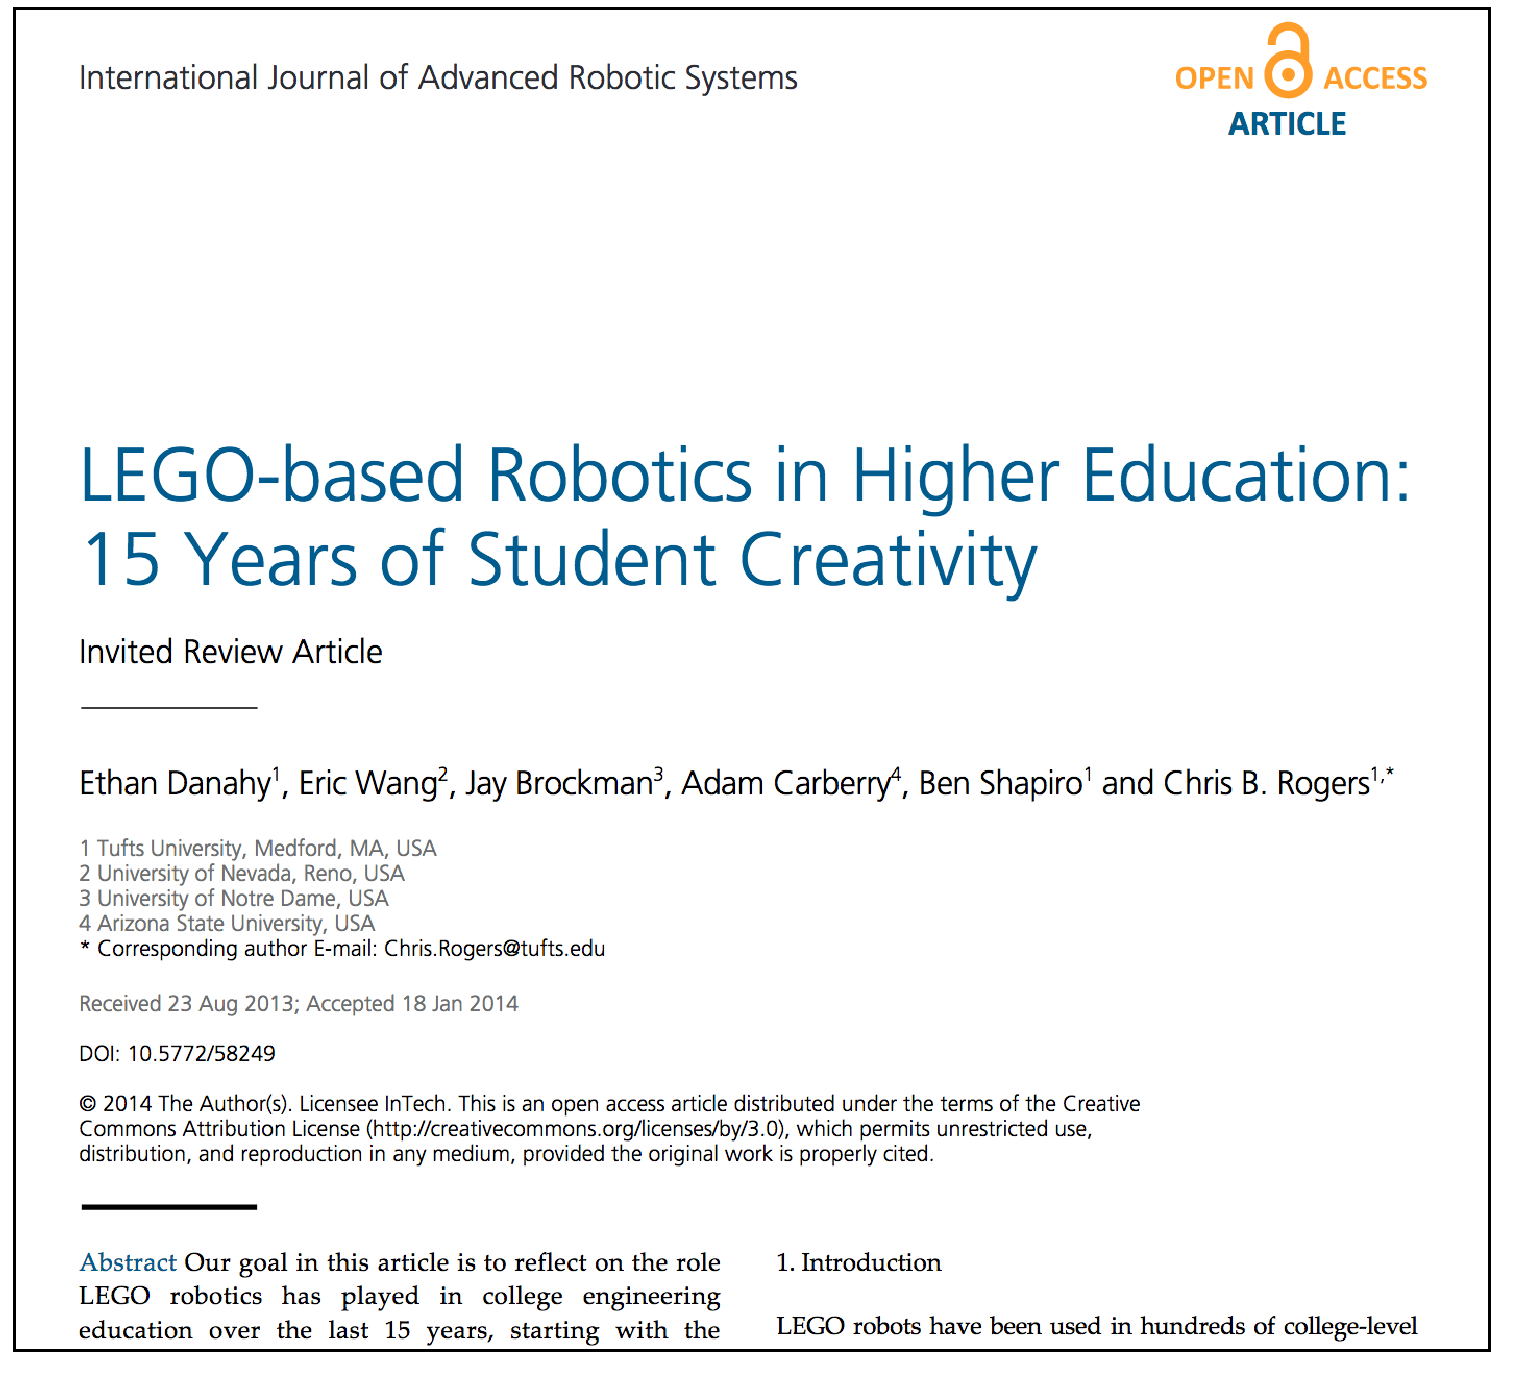
\includegraphics{article}}
  \caption{Artikkel publisert i en journal.} 
  \label{fig:article}
\end{figure}

\newpage

På grunn av antall forfattere, ville denne artikkelen
fått {\em tag}'en  \fbox{\tt  Dan\_et\_al.2014} i 
.bib-fila. Husk at du ikke benytter linjeskift i
  oppramsingen av {\em authors}, se under

\begin{boxedminipage}{200mm}
{\footnotesize{
\begin{verbatim}
@Article{Dan_et_al.2014,
  author = {Ethan Danahy and Eric Wang and Jay Brockman and Adam Carberry and Ben Shapiro and Chris B. Rogers},
  title = {LEGO-based Robotics in Higher Education: 15 Years of Student Creativity},
  journal = {Int J Adv Robot Syst},
  year = {2014},
  pages = {1--15},
  volume = {11},
  number = {27},
  note = {doi: 10.5772/58249}
}
\end{verbatim}
}}
\end{boxedminipage}

Legg merke til at journalens navn er forkortet til {\tt Int J Adv
  Robot  Syst}, og at sidenummerområde bruker 2 bindestreker.



Den fullstendige beskrivelsen av {\tt @Article} er

\begin{verbatim}
@Article{,
  author = 	 {},
  title = 	 {},
  journal = 	 {},
  year = 	 {},
  OPTkey = 	 {},
  OPTvolume = 	 {},
  OPTnumber = 	 {},
  OPTpages = 	 {},
  OPTmonth = 	 {},
  OPTnote = 	 {},
  OPTannote = 	 {}
}
\end{verbatim}

\newpage

\subsection{\fbox{\tt @InProceedings}}
{\tt @InProceedings} er en artikkel som er 
  presentert ved en konferanse. Et eksempel er denne
  {\color{red}\href{https://bit.ly/2AvqFO8}{https://bit.ly/2AvqFO8}}
  som handler om bruk av LEGO Mindstorms, og som ble presentert på IFAC
  sin 18. verdenskonferanse i Milano. Ved å trykke på
  {\color{red}{Download full text in PDF}} vil du se at artikkelen ser
  slik ut.
\begin{figure}[H]
  \centering
  \scalebox{0.5}{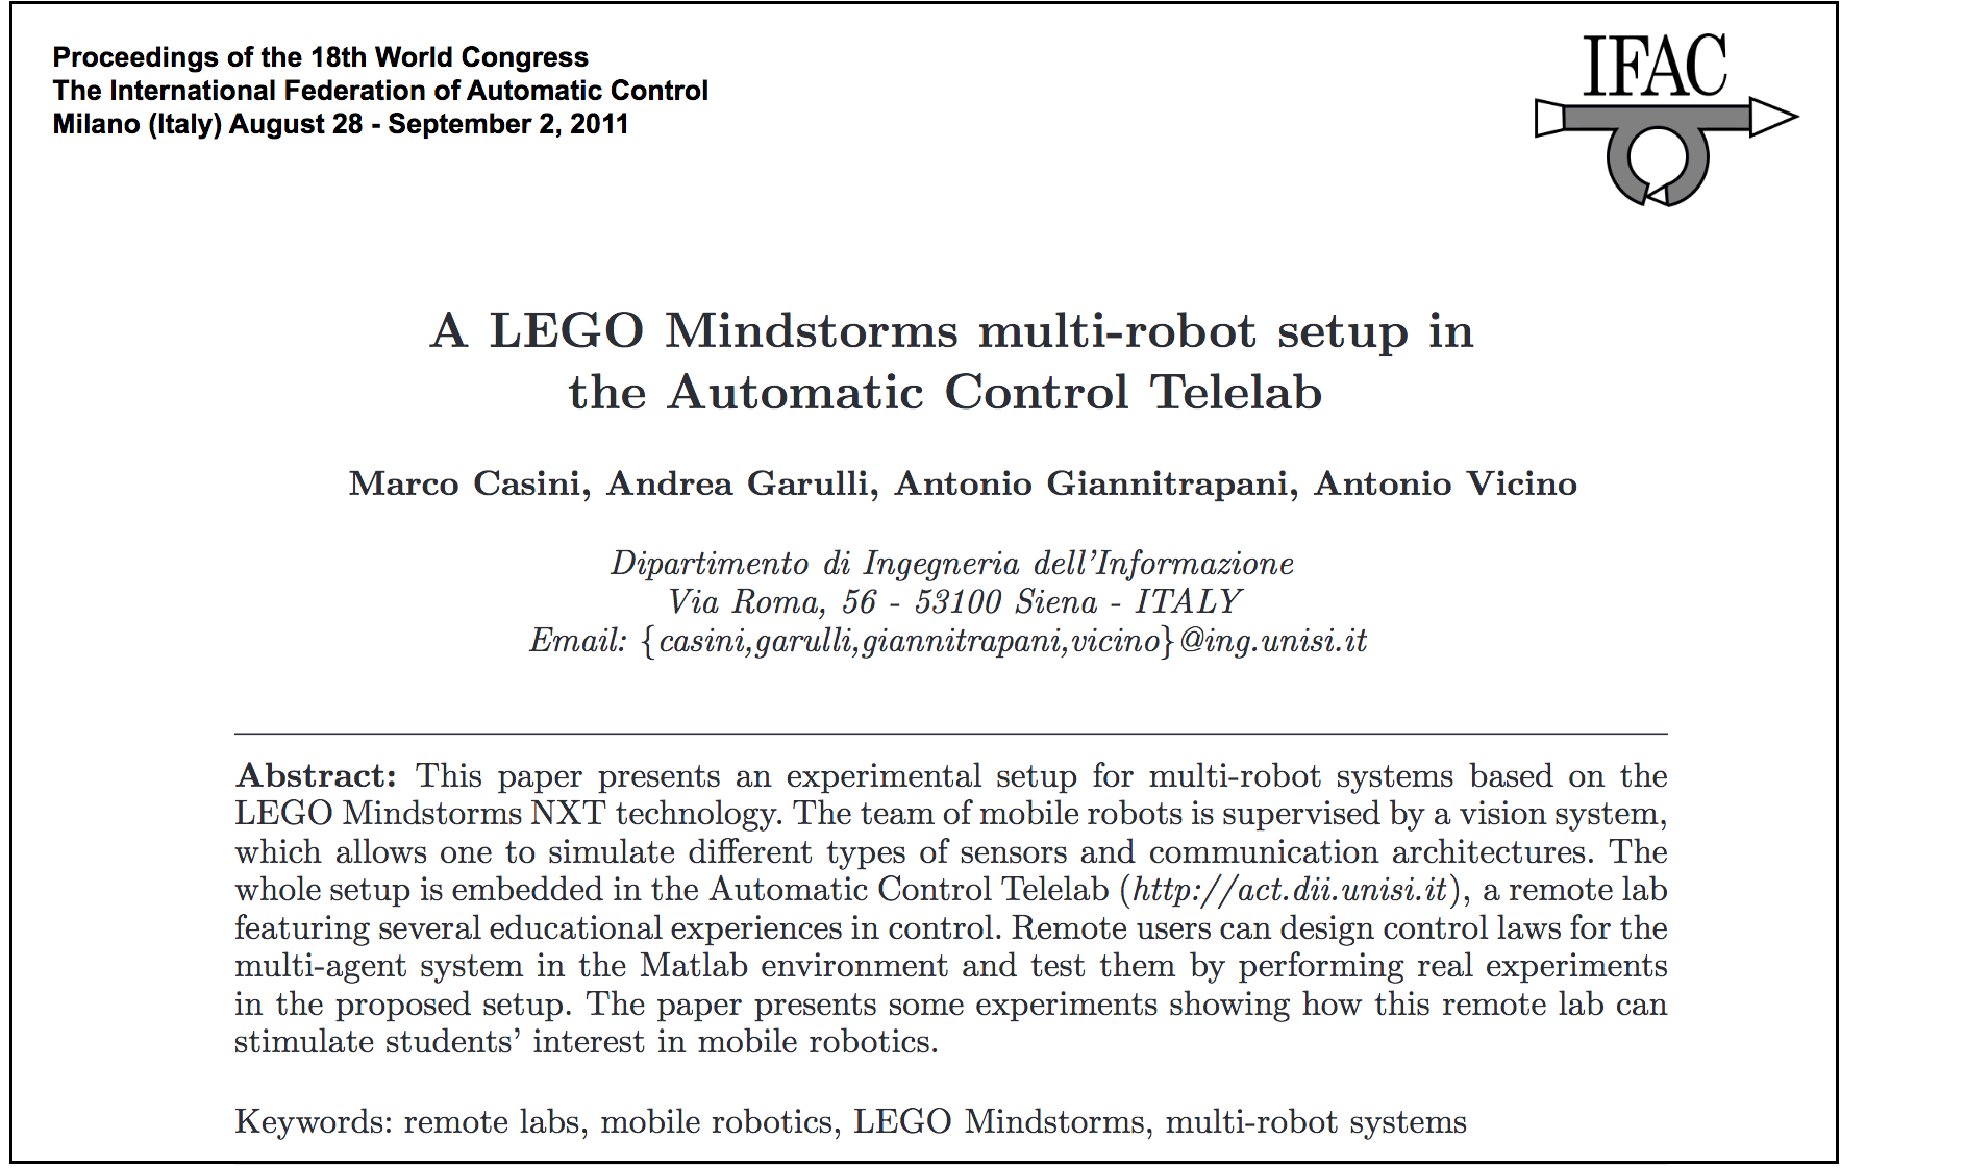
\includegraphics{proceedings}}
  \caption{Artikkel presentert ved konferanse.} 
  \label{fig:proceedings}
\end{figure}

\newpage

Siden denne artikkelen bare hadde 4 forfattere, 
får den {\em tag}'en  \fbox{\tt  CasGarGiaVic2011}
i .bib-fila, se under

\begin{boxedminipage}{160mm}
{\footnotesize{
\begin{verbatim}
@InProceedings{CasGarGiaVic2011,
  author = {Marco Casini and Andrea Garulli and Antonio Giannitrapani and Antonio Vicino},
  title = {A LEGO Mindstorms multi-robot setup in the Automatic Control Telelab},
  booktitle = {Proceedings of the 18th World Congress},
  year = {2011},
  pages = {9812--9817},
  organization = {IFAC},
}
\end{verbatim}
}}
\end{boxedminipage}

Den fullstendige beskrivelsen av {\tt InProceedings} er:

\begin{verbatim}
@InProceedings{,
  author = 	 {},
  title = 	 {},
  OPTcrossref =  {},
  OPTkey = 	 {},
  OPTbooktitle = {},
  OPTyear = 	 {},
  OPTeditor = 	 {},
  OPTvolume = 	 {},
  OPTnumber = 	 {},
  OPTseries = 	 {},
  OPTpages = 	 {},
  OPTmonth = 	 {},
  OPTaddress = 	 {},
  OPTorganization = {},
  OPTpublisher = {},
  OPTnote = 	 {},
  OPTannote = 	 {}
}
\end{verbatim}

\newpage

\subsection{\fbox{\tt @PhDThesis} og \fbox{\tt @MastersThesis}}
Dersom du skal referere til andre studenters
forskningsarbeid, kan du bruke 
{\tt @PhDThesis} og {\tt @MastersThesis}. Som du ser under nedenfor, 
benytter disse identiske elementer.
Det finnes også en 
{\tt @Thesis} som kan brukes for bacheloroppgaver.




\begin{verbatim}
@PhdThesis{,
  author = 	 {},
  title = 	 {},
  school = 	 {},
  year = 	 {},
  OPTkey = 	 {},
  OPTtype = 	 {},
  OPTaddress = 	 {},
  OPTmonth = 	 {},
  OPTnote = 	 {},
  OPTannote = 	 {}
}
\end{verbatim}

\begin{verbatim}
@MastersThesis{,
  author = 	 {},
  title = 	 {},
  school = 	 {},
  year = 	 {},
  OPTkey = 	 {},
  OPTtype = 	 {},
  OPTaddress = 	 {},
  OPTmonth = 	 {},
  OPTnote = 	 {},
  OPTannote = 	 {}
}
\end{verbatim}

\newpage
\section{Referering til litteratur, \fbox{\tt $\backslash$cite\{ \}}}
For å referere til de forskjellige litteraturelementene i 
\fbox{\tt referanser.bib}, må du bruke \fbox{\tt
  $\backslash$cite}-kommandoen som vist i følgende eksempel.

\begin{boxedminipage}{\textwidth}
\begin{verbatim}
Som vist i~\cite{Dre2019} kan numerisk integrasjon benyttes til ...
\end{verbatim}
\end{boxedminipage}

og denne vil fremstå slik:

Som vist i~\cite{Dre2019} kan numerisk integrasjon benyttes til ...


Det er vanlig at referanselisten kommer etter konklusjonen.
For å få dette til må du inkludere følgende
kodelinjer i hovedfilen rett etter konklusjonskapittelet:

\begin{boxedminipage}{\textwidth}
\begin{verbatim}
\bibliographystyle{plain}
\bibliography{referanser.bib}
\addcontentsline{toc}{chapter}{Bibliografi} 
\end{verbatim}
\end{boxedminipage}

Første linje forteller hvilken stil du ønsker å bruke. 
Stilen som heter \fbox{\tt plain} plasserer et tall foran hver
referanse i referanselista, og det er dette tallet som vises i
teksten. 

Andre linje forteller {\LaTeX} hvilken .bib-fila som skal
benyttes. Her kan det stå flere filnavn.

Siste linje legger til ``Bibliografi''-kapittelet i innholdsfortegnelsen.






\chapter{Litt om ligninger}\label{kap:ligninger}

\section{Bruk av \fbox{\tt equation}-miljøet}\label{delkap:equation}
For å skrive ligninger i {\LaTeX} brukes \fbox{\tt equation}-miljøet
på følgende måte: 

\begin{boxedminipage}{\textwidth}
\begin{verbatim}
\begin{equation}
  \label{eq:sinus}
  y(t)=\sin(\omega t)
\end{equation}
\end{verbatim}
\end{boxedminipage}

som resulterer i følgende ligning hvor ligningsnummeret~\eqref{eq:sinus}
kommer automatisk opp på høyre side av ligningen.
\begin{equation}
  \label{eq:sinus}
  y(t)=\sin(\omega t)
\end{equation}


\section{Bruk av \fbox{\tt align}-miljøet}\label{delkap:align}
For å sette flere ligninger over hverandre er 
\fbox{\tt align} nyttig. Denne benytter tegnet {\&} for å markere
hvilken plass i ligningene som skal {\em alignes}.
I  eksemplet under er det likhetstegnet og 
{\tt $\backslash$downarrow}  som skal stå
over hverandre. For hver linjeslutt {\color{red}(utenom den siste
  linjen)} må du indikere det med
$\backslash\backslash$.

\begin{boxedminipage}{\textwidth}
\begin{verbatim}
\begin{align}
  y(t) & = \sin(\omega t) \tag{\ref{eq:sinus}} \\
       & \downarrow \notag \\
  y(t) & = \cos \Bigl( \omega t - \frac{\pi}{2} \Bigr) 
         \label{eq:cosinus}
\end{align}
\end{verbatim}
\end{boxedminipage}
 
Resultatet av koden er vist under
\begin{align}
  y(t) & = \sin(\omega t) \tag{\ref{eq:sinus}}\\
        & \downarrow \notag\\
  y(t) & = \cos \Bigl(\omega t - \frac{\pi}{2}\Bigr) \label{eq:cosinus}
\end{align}
Noen kommentarer til resultatet:
\begin{itemize}
\item Legg merke til at ligningsnummeret~\eqref{eq:sinus} til den øverste ligningen er det
  samme i ligningen i forrige delkapittel, og dette er gjort
  ved å bruke \fbox{\tt $\backslash$tag\{\}}-funksjonen som manuelt {\em
    tag}'er en ligning med ligningsnummeret til en annen ligning ved
  bruk av \fbox{\tt $\backslash$ref\{\}}-funksjonen fra
  kapittel~\ref{delkap:ref}. Denne måten å lage ligningsnummer på
  brukes bare når ligningene er identiske, slik som de er i dette
  tilfelle. 

\item Videre ser du at {\tt $\backslash$downarrow}-pilen 
  ikke har ligningsnummer (som er jo logisk), og
  dette løses med \fbox{\tt $\backslash$notag}-funksjonen.

\item Legg også merke til at selve sinus- og cosinusfunksjonene i ligningene~\eqref{eq:sinus} 
  og \eqref{eq:cosinus} 
  ser ut som vanlig stående tekst siden de skrives med kommandoen 
  \fbox{\tt $\backslash$sin} og \fbox{\tt $\backslash$cos}.

\item Legg merke til at siste linje IKKE skal ha
  $\backslash\backslash$ på siste linje. Dersom du glemmer dette, vil det dukke opp
  en tom linje med ligningsnummer.
\end{itemize}



\section{Bruk av matematikkmodus i rapporttekst, \$x\$}
Når du i teksten skriver om variabler som brukes i ligningene må du
huske å skrive disse i matematikkmodus, det vil si med dollartegn
foran og etter symbolet. I ligning~\eqref{eq:sinus} brukes for eksempel tiden
$t$, hvor {\LaTeX}-koden for å skrive tidsvariabel i matematikkmodus er \fbox{\tt \$t\$}.

Unngå å skrive ligninger i selve teksten. Dette fordi det ofte er
vanskelig å lese, og du kan heller ikke referere til ligningen senere
i teksten. Bruk derfor {\tt $\backslash$begin\{equation\}} og 
  {\tt $\backslash$end\{equation\}} for alle ligninger.


\section{Bruk av vanlig tekst i ligninger, \fbox{\tt $\backslash$mathrm\{ \}}}
Det er ikke ofte du har bruk for å skrive vanlig tekst i ligningene,
men skal du gjøre dette kan du bruke 
\fbox{\tt $\backslash$mathit\{\}} eller 
\fbox{\tt $\backslash$mathrm\{\}} kommadoene. 
Et eksempel på dette er vist i ligning~\eqref{eq:sin_og_cos}, hvor 
\fbox{\tt $\backslash$underbrace\{\}}-kommandoen og 
\fbox{\tt $\backslash$hspace*\{\}}-kommandoen  er brukt i \fbox{\tt
  align}-miljøet. 

\begin{boxedminipage}{160mm}
\begin{verbatim}
\begin{align}
  y(t) & = \underbrace{\sin(\omega t)} 
          + \underbrace{\cos(2 \pi f t)} \label{eq:sin_og_cos}\\
       & \hspace*{5mm}\mathrm{Roman font} 
         \hspace*{7mm}\mathit{Italic~font}\notag
\end{align}
\end{verbatim}
\end{boxedminipage}

som gir følgende resultat (legg merke til at du må bruke tilde for å
lage mellomrom)
\begin{align}
  y(t)  &= \underbrace{\sin(\omega t)} 
          + \underbrace{\cos(2 \pi f t)}   \label{eq:sin_og_cos} \\
          & \hspace*{5mm}\mathrm{Roman font}
            \hspace*{7mm}\mathit{Italic~font} \notag
\end{align}

\section{Bruk av \fbox{\tt $\backslash$hspace*\{ \}}}\label{delkap:hspace}
I eksempelet over ble kommandoen \fbox{\tt $\backslash$hspace*\{\}}
brukt.  Denne betyr {\em horisontal space}, og
tilsvarende finnes det også \fbox{\tt $\backslash$vspace*\{\}} betyr 
{\em vertical  space}. For at ikke {\LaTeX} skal ignorere dine ønsker
å horisontal og vertikal avstand, MÅ du bruke {\tt *} slik som vist i
koden over. 

Husk at du kan flytte både til høyre/venstre og ned/opp ved å
bruke hhv. positive og negative verdier, og du kan angi forflytningen
i mm, cm, eller punkter pt.




\chapter{Litt om figurer}\label{kap:figurer}
 
\section{Bruk av \fbox{\tt figure}-miljøet}\label{delkap:figure}
For å inkludere figurer bruker du {\tt figure}-miljøet på følgende
måte

\begin{boxedminipage}{\textwidth}
\begin{verbatim}
\begin{figure}[H]
  \centering
  \scalebox{0.6}{\includegraphics{figurfilnavn}}
  \caption{Figurtekst som beskriver hva vi ser i figuren.} 
  \label{fig:xxxxx}
\end{figure}
\end{verbatim}
\end{boxedminipage}

Den store H-en etter {\tt $\backslash$begin\{figure\}} betyr her,
eller {\em here} på engelsk. Det betyr at figuren plasseres akkurat
der den står i teksten. For å bruke \fbox{[H]} må du inkludere pakken
\fbox{\tt here} på følgende måte \fbox{\tt $\backslash$usepackage\{here\}}.

Dersom du vil at {\LaTeX} skal bestemme plasseringen av figuren ved
kompilering, kan du f.eks. skrive \fbox{[ht]} som betyr at du
\underline{ønsker} at den skal plasseres her og helst mot toppen
øverst på en side. Ved å spesifisere slik havner ofte figuren en helt
annen plass i rapporten, og det er litt slitsomt.

Kommandoen {\tt $\backslash$scalebox\{0.6\}} skalerer figuren til 60\%
av opprinnelig størrelse. 

For oversiktens skyld pleier jeg ofte å la {\tt xxxxx} i figur-{\em tag}'en
\fbox{\tt fig:xxxxx} være det samme som navnet på figurfila, dvs
\fbox{\tt $\backslash$label\{fig:figurfilnavn\}}

\section{MATLAB-figurer}
\subsection{Format og størrelse}
For at MATLAB-figurer skal være lesbar i rapporten må du bruke \fbox{png}-
eller \fbox{pdf}-formatet. Bruker du \fbox{jpg} vil detaljene smøres
utover og  det er ofte umulig å lese ut informasjon av slike
figurer. {\color{red}Inntrykket av rapporten blir dermed dårlig. }
Dersom du lagrer en MATLAB-figur til pdf-formatet ved å bruke
\fbox{\tt File}-menyen som vist i figur~\ref{fig:save_as}, vil det
komme mye tomrom med i figuren som 
vist i  figur~\ref{fig:daarlig}. 

\begin{figure}[H]
  \centering
  \scalebox{0.55}{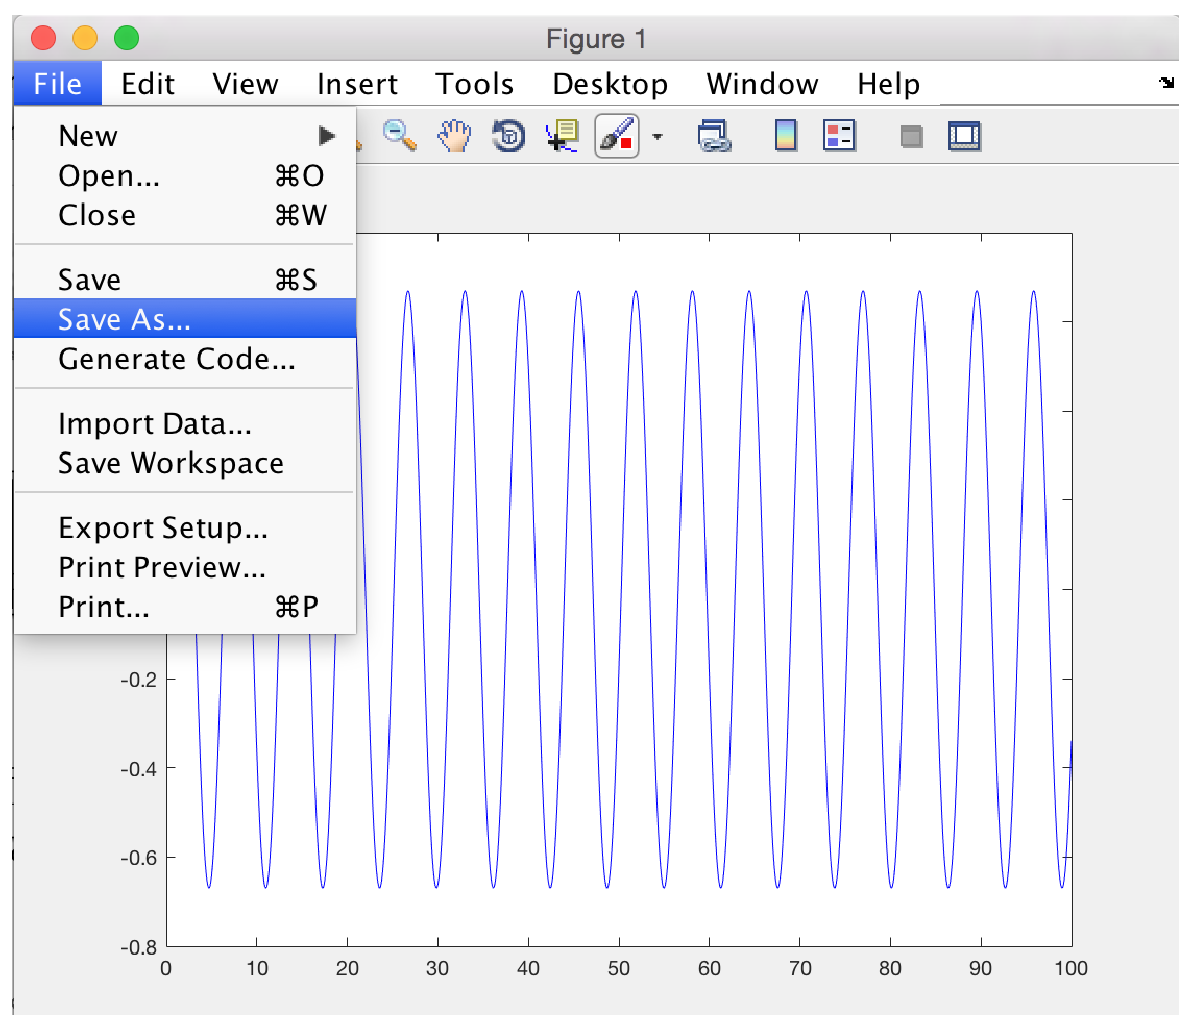
\includegraphics{save_as}}
  \caption{Dersom du lagrer figuren i pdf-format via denne menyen,
    blir det mye hvitt tomrom rundt figuren, se figur~\ref{fig:daarlig}.} 
  \label{fig:save_as}
\end{figure}

\begin{figure}[H]
  \centering
  \scalebox{0.55}{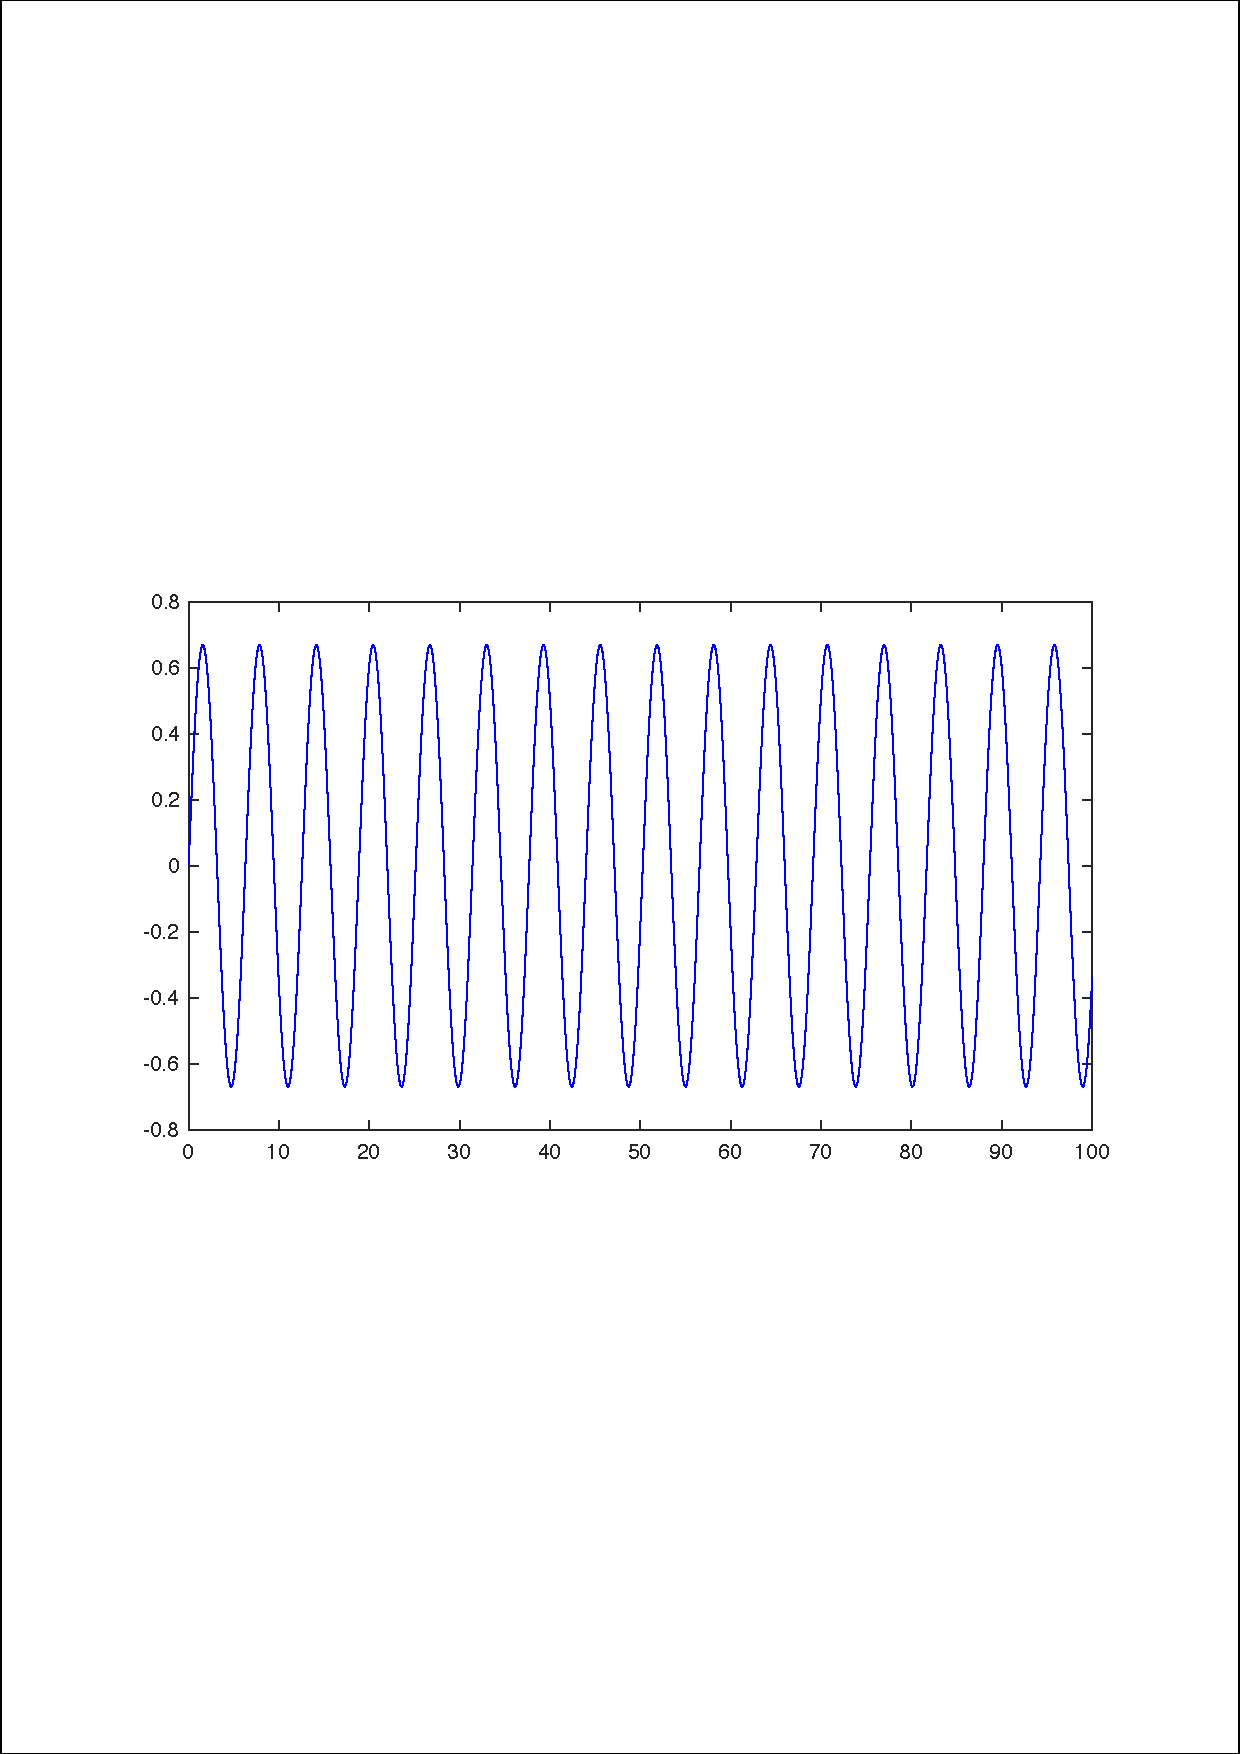
\includegraphics{daarlig_fig}}
  \caption{Dårlig figur med mye hvitt tomrom. Det er lagt
    på en ramme for å vise hvor mye hvitt tomrom som kommer med.} 
  \label{fig:daarlig}
\end{figure}
{\color{red}Dette er med andre ord ikke måten å lage pdf-figurer på.}

\subsection{Funksjonen \fbox{\tt SaveMyFigure.m}}
For at du effektivt skal lage pdf-figurer uten dette store hvite feltet, finner
du i mappen \fbox{MineFunksjoner} en funksjon som heter
\fbox{SaveMyFigure.m}. Denne kaller du med følgende kode i {\em
  Command Window} {\color{red}(husk å stå i den mappen hvor du ønsker
  figuren lagret):}

\begin{boxedminipage}{\textwidth} 
\begin{verbatim}
SaveMyFigure(gcf,'figurnavn')
\end{verbatim}
\end{boxedminipage}

hvor \fbox{\tt gcf} står for \fbox{\tt get current window}, som betyr
at funksjonen lager figur av den MATLAB-figuren du sist trykket med
musepekeren i. Funksjonen lager både en .pdf-versjon
og en .fig-versjon, hvor .fig-versjonen  kan åpnes i ettertid slik at
du ved en 
senere anledning kan endre/legge til ting i figuren.
Koden for funksjonen er i sin helhet gjengitt i
kodeutdrag~\ref{kode:SaveMyFigure}. På side~\pageref{side:kodelisting}
vises det hvordan du kan inkludere kode på denne måten.


\lstinputlisting[caption=Funksjonen {\tt SaveMyFigure.m},
                             label=kode:SaveMyFigure]{SaveMyFigure.m}

\subsection{Effekten av vindusstørrelse {\em før} lagring}
Dersom størrelsen på figuren i forhold til skjermstørrelsen er stor
slik som vist i figur~\ref{fig:god_stort_vindu}, vil resultatet etter lagring med funksjonen
{\tt SaveMyFigure} bli som i figur~\ref{fig:god}
hvor du er at tallene langs x- og y-aksen i figur~\ref{fig:god} nesten
uleselige. 
Dette skyldes at MATLAB-figuren i utgangspunktet dekket nesten hele
skjermen som vist i figur~\ref{fig:god_stort_vindu}.

\begin{figure}[H]
  \centering
  \scalebox{0.22}{\includegraphics{god_stort_vindu}}
  \caption{MATLAB-figuren fyller ut nesten hele skjermen.} 
  \label{fig:god_stort_vindu}
\end{figure}
\begin{figure}[H]
  \centering
  \scalebox{0.21}{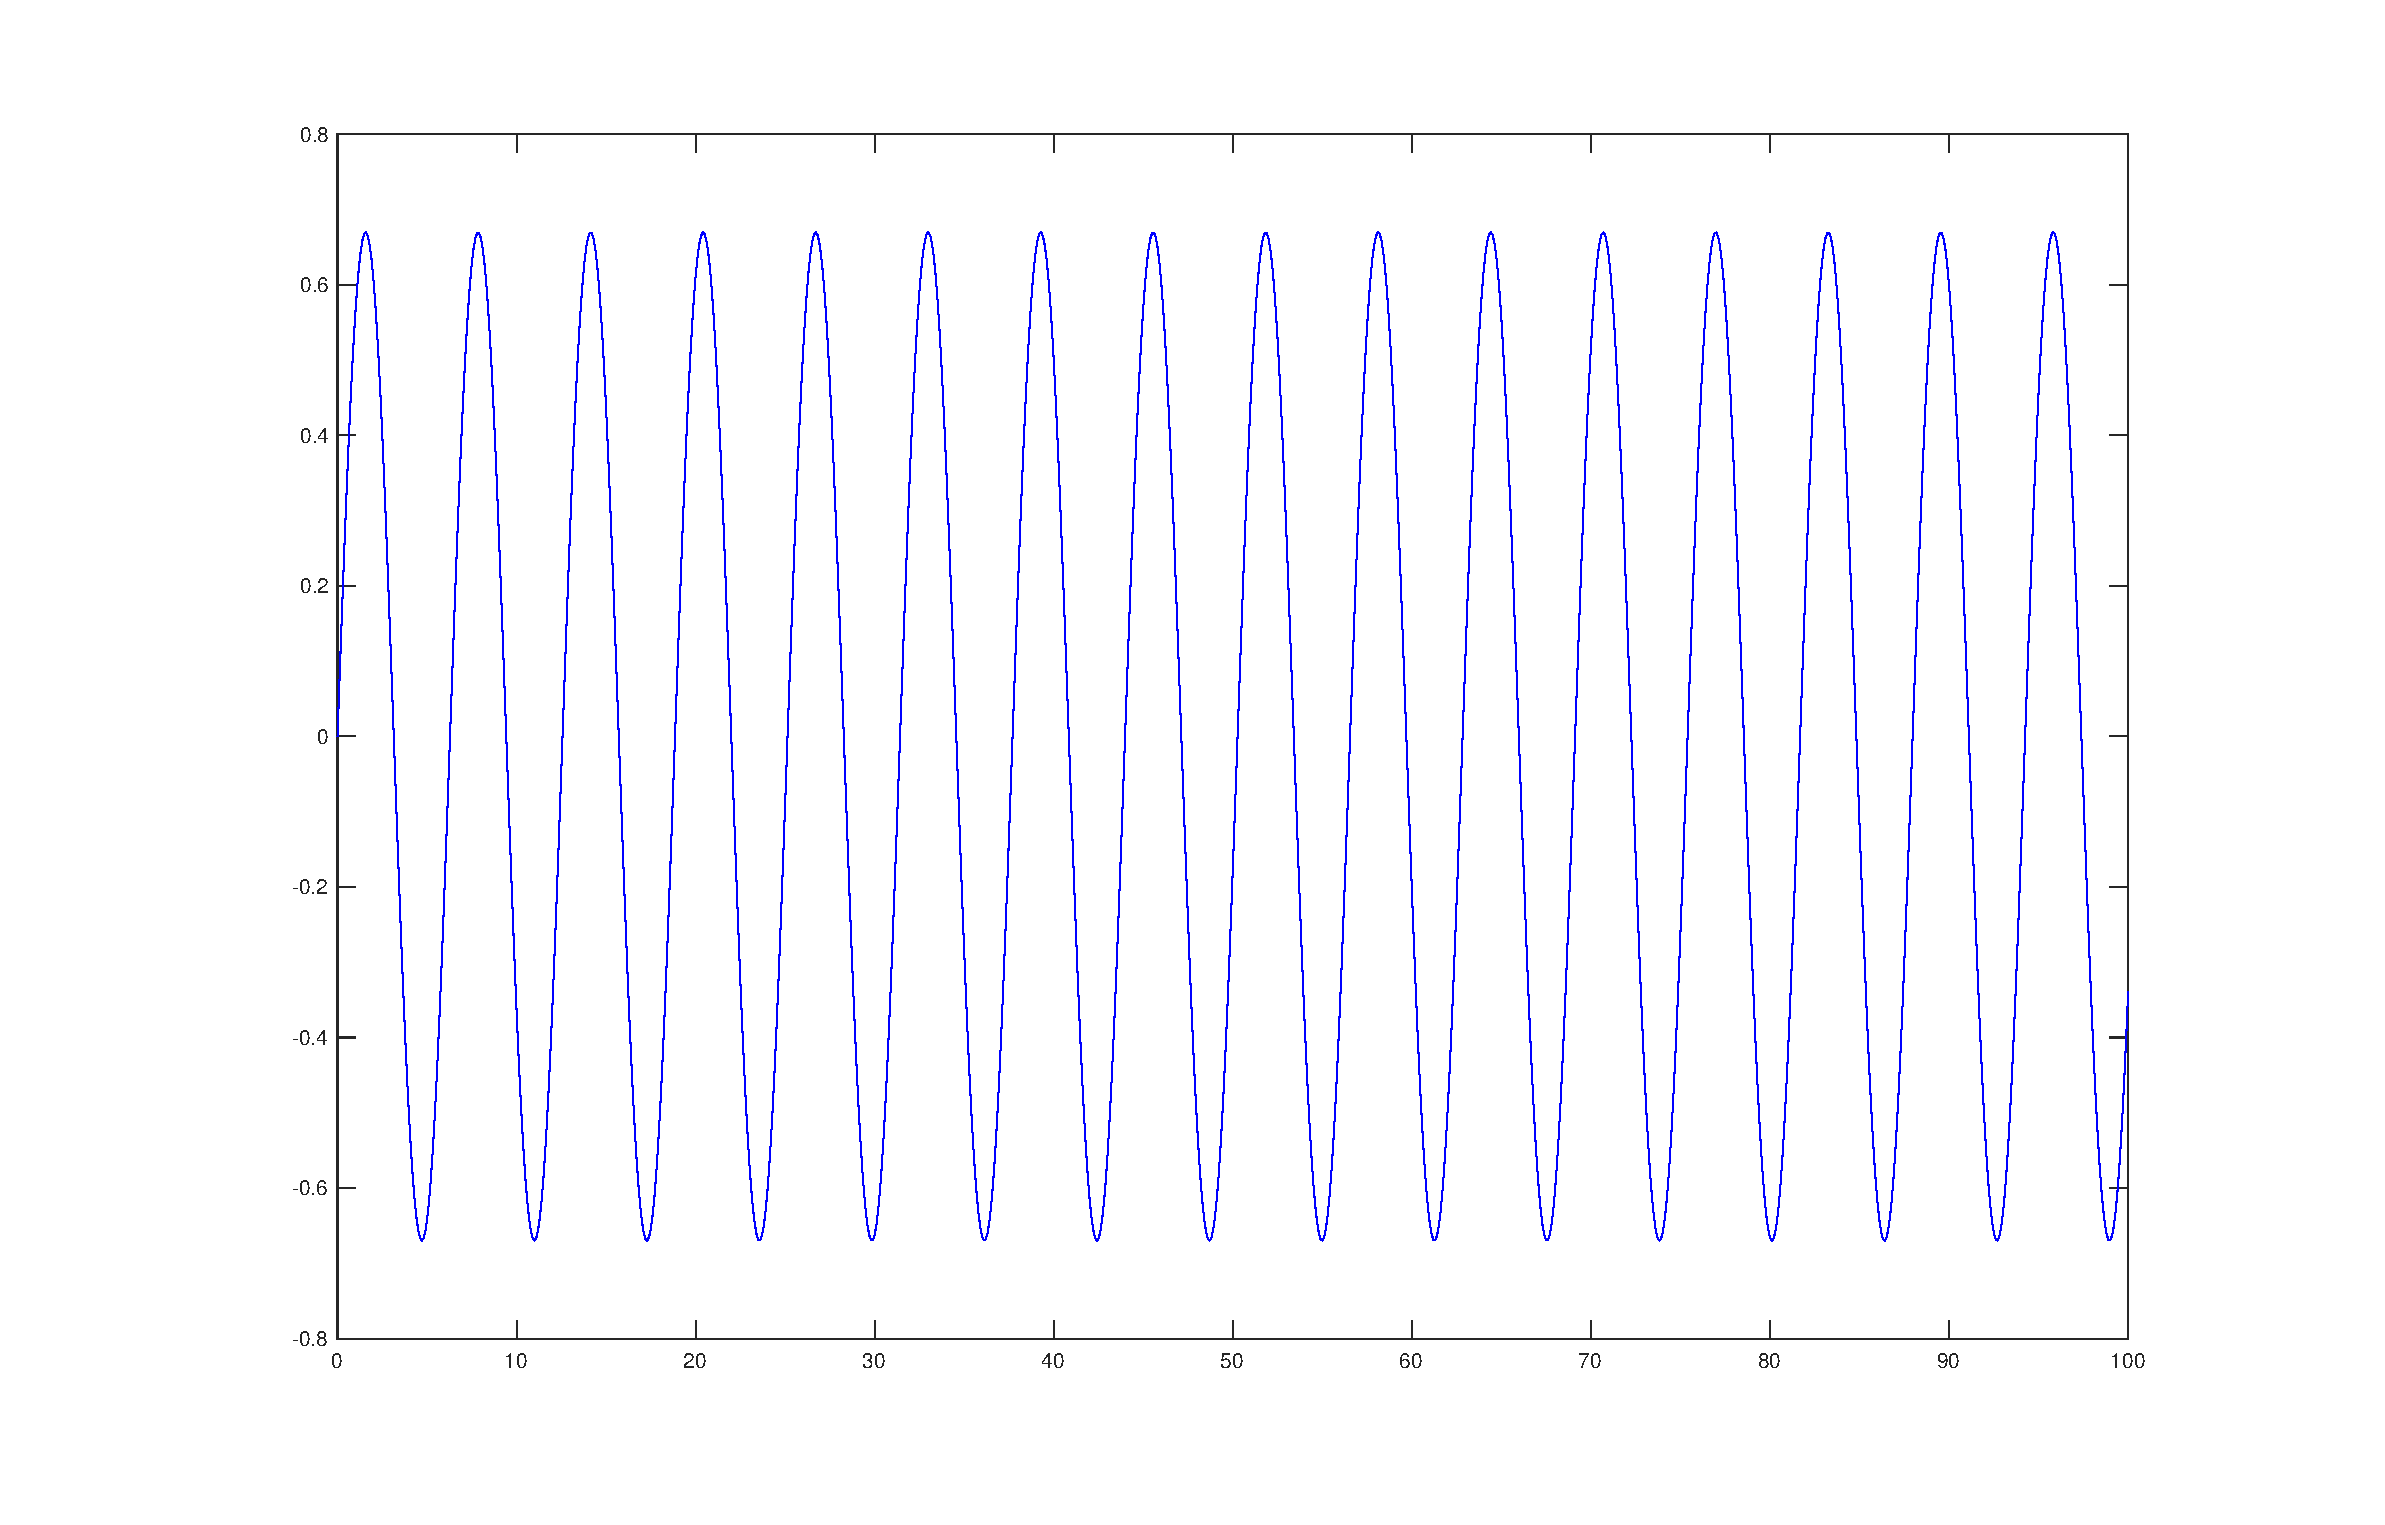
\includegraphics{god}}
  \caption{Slik blir pdf-versjonen av MATLAB-figuren i
    figur~\ref{fig:god_stort_vindu} når lagres med {\tt
      SaveMyFigure}-funksjonen. Tekstfonten er altfor liten, og
    tallverdiene på aksene er uleselig.}  
  \label{fig:god}
\end{figure}

Dersom du reduserer størrelsen på selve MATLAB-figurvinduet 
som vist i figur~\ref{fig:god_lite_vindu} før du lagrer, vil fontstørrelsen på
aksene fremstå som relativt mye større i forhold til selve figuren. 
\begin{figure}[H]
  \centering
  \scalebox{0.22}{\includegraphics{god_lite_vindu2}}
  \caption{MATLAB-figuren er redusert i størrelse før lagring med {\tt
      SaveMyFigure}-funksjonen.} 
  \label{fig:god_lite_vindu}
\end{figure}
Konsekvensen av dette er at leseren
faktisk er i stand til å se tallene, se figur~\ref{fig:god2}.
\begin{figure}[H]
  \centering
  \scalebox{0.58}{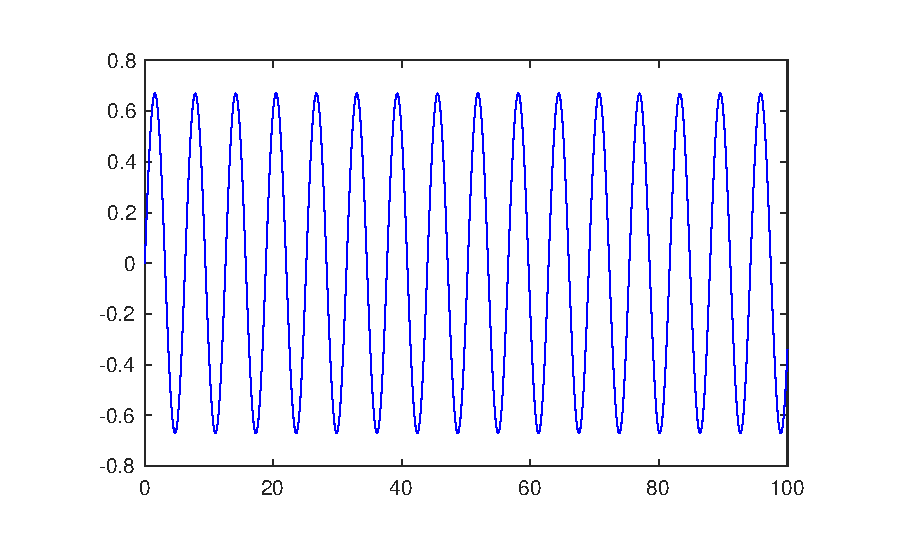
\includegraphics{god2}}
  \caption{MATLAB-figuren i figur~\ref{fig:god_lite_vindu} lagret med {\tt
      SaveMyFigure}-funksjonen. Legg merke til den fornuftige
    fontstørrelsen  på x- og  y-aksen.} 
  \label{fig:god2}
\end{figure}

\subsection{Inkludering av {\LaTeX}-tekst i MATLAB-figurene} 
En figur skal \underline{alltid} ha tekstbasert 
indikering av hva som vises på x- og y-aksene.  I figurene i forrige
delkapittel var dette helt fraværende, og derfor vises det nå
hvordan du kan få {\LaTeX}-font på tekststrengene. Utgangspunktet er
koden for selve sinuskurven i figur~\ref{fig:god2}, men hvor det er
lagt til \fbox{\tt title}, \fbox{\tt xlabel} og \fbox{\tt ylabel} med
{\LaTeX}-font og fontstørrelse 16.

\begin{boxedminipage}{\textwidth}
\begin{verbatim}
t=0:0.1:100;
y_1=2/3*sin(t);
plot(t,y_1)
title('$y_1(t)=\frac{2}{3}\sin(t)$','Interpreter','latex');
xlabel('$t$ [s]','interpreter','latex')
ylabel('$y_1(t)$','interpreter','latex')
\end{verbatim}
\end{boxedminipage}

\begin{figure}[H]
  \centering
  \scalebox{0.58}{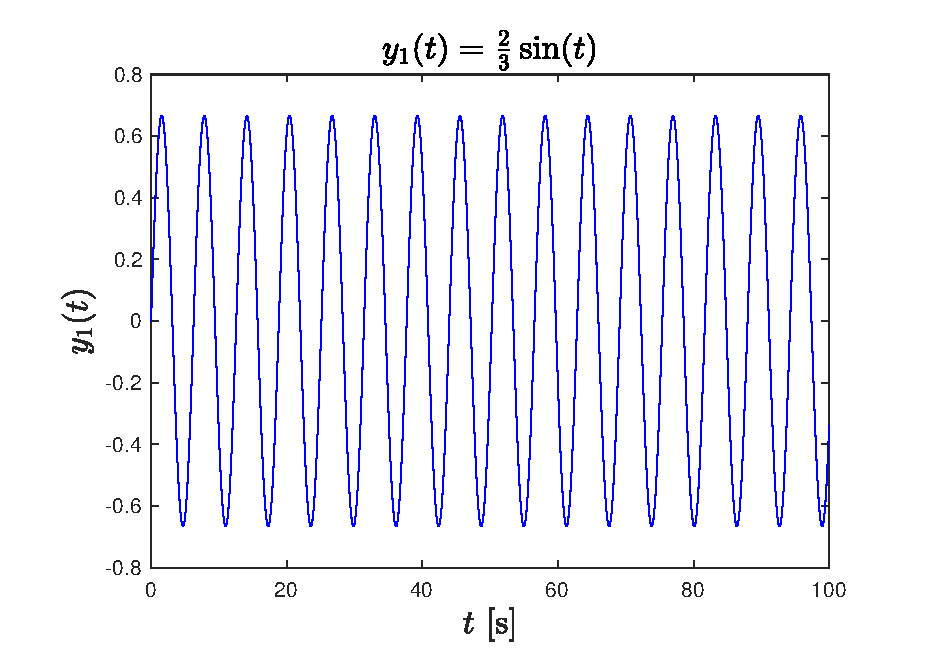
\includegraphics{god3}}
  \caption{Eksempel på en god MATLAB-figur med tydelige, lesbare
    akseverdier og tekst på x- og y-akse, med figurtittel.} 
  \label{fig:god3}
\end{figure}




\chapter{Litt om tabeller}\label{kap:tabeller}

\section{Bruk av \fbox{table}- og \fbox{tabular}-miljøene}

Tabeller kan være vanskelig i \LaTeX. Under er det vist noen eksempler
på tabeller slik at du kan bruke de som et utgangspunkt for dine egne
tabeller.
Husk at
tabelltekst skal stå over tabellen, imotsetning til figurtekst som
står under.

Følgende kode gir tabell~\ref{tab:enkel_tab}
som resultat. 

\begin{boxedminipage}{\textwidth}
\begin{verbatim}
\begin{table}[H]
  \centering
  \caption{Enkel tabell.}
  \begin{tabular}{|l|r c|r|c|}\hline
    Venstrejustert & Høyrejustert & Sentrert 
    &  Høyrejustert & Sentrert \\\hline\hline 
    1.3434 & 0.55677 & 0.2 & 1.45   & 0.3     \\
    2.5667 & 0.66    & 0.4 & 100.01 & 1.43435 \\\hline
  \end{tabular}
  \label{tab:enkel_tab}
\end{table}
\end{verbatim}
\end{boxedminipage}

\begin{table}[H]
  \centering
  \caption{Enkel tabell.}
  \begin{tabular}{|l|r c|r|c|}\hline
    Venstrejustert & Høyrejustert & Sentrert 
    &  Høyrejustert & Sentrert \\\hline\hline 
    1.3434 & 0.55677 & 0.2 & 1.45     & 0.3  \\
    2.5667 & 0.66       & 0.4 & 100.01 & 1.43435  \\\hline
  \end{tabular}
  \label{tab:enkel_tab}
\end{table}
Hvert element i tabellen skilles med et \&-tegn, og det kan være
nyttig å organiserer disse \&-tegnene oppå hverandre slik at tabellen
er lettere å lese i .tex-fila.  


Detaljene som er vist i følgende linje i koden over

\begin{boxedminipage}{\textwidth}
\begin{verbatim}
  \begin{tabular}{|l|r c|r|c|}\hline
\end{verbatim}
\end{boxedminipage}

betyr at tabellen skal inneholde 5 kolonner hvor
\begin{itemize}
\item  symbolet \fbox{|} betyr loddrett tabellstrek, 
\item \fbox{\tt l} betyr {\em left} og dermed venstrejustert
\item \fbox{\tt r} betyr {\em right} og dermed høyrejustert
\item \fbox{\tt c} betyr {\em center} og dermed sentrert
\item kommanoden \fbox{\tt $\backslash$hline} betyr {\em horisontal
    line} og dermed vannrett tabellstrek
\end{itemize}

\newpage

Koden for en litt mer avansert tabell er vist under og i 
tabell~\ref{tab:avansert_tab}. Denne inneholder både 
{\tt $\backslash$multirow}, 
{\tt $\backslash$multicolumn}, 
{\tt $\backslash$cellcolor}, 
 og{\tt $\backslash$cline}. 

\begin{boxedminipage}{160mm}
\begin{verbatim}
\begin{table}[H]
  \centering
  \renewcommand{\arraystretch}{1.2}
  \caption{Parametre brukt i simuleringen.}
  \begin{tabular}{|c||c|c||c|c|c|}\hline
    \multirow{2}{*}{Controller} & \multicolumn{2}{c||}{Variables} 
                                & \multicolumn{3}{c|}{Parameters}\\
    \cline{2-6}
    no. & \cellcolor[gray]{0.8} & & & &\\[-4mm]
          & \cellcolor[gray]{0.8}  $h_{high}$ &$u_{high}$  & $k_{s}^{u}$  
                                & $V_{max}^{u}$ &    $K_{M}^{u}$  \\[1mm]\hline
    1 & \cellcolor[gray]{0.8} 0.55 & 0.49 & 0.01 & 0.0071  & 0.137 \\
    2 & \cellcolor[gray]{0.8} 0.66 & 0.47 & 0.01 & 0.0177  & 0.797 \\\hline
  \end{tabular}
  \label{tab:avansert_tab}
\end{table}
\end{verbatim}
\end{boxedminipage}

\begin{table}[H]
  \centering
  \renewcommand{\arraystretch}{1.2}
  \caption{Parametre brukt i simuleringen.}
  \begin{tabular}{|c||c|c||c|c|c|}\hline
    \multirow{2}{*}{Controller} & \multicolumn{2}{c||}{Variables} & \multicolumn{3}{c|}{Parameters}\\
    \cline{2-6}
    no. & \cellcolor[gray]{0.8} & & & &\\[-4mm]
          & \cellcolor[gray]{0.8}  $h_{high}$ &$u_{high}$  & $k_{s}^{u}$  
                                & $V_{max}^{u}$ &    $K_{M}^{u}$  \\[1mm]\hline
    1 & \cellcolor[gray]{0.8} 0.55 & 0.49 & 0.01 & 0.0071  & 0.137 \\
    2 & \cellcolor[gray]{0.8} 0.66 & 0.47 & 0.01 & 0.0177  & 0.797 \\\hline
  \end{tabular}
  \label{tab:avansert_tab}
\end{table}

Legg merke til at kommadoen
{\tt $\backslash$renewcommand\{$\backslash$arraystretch\}\{1.2\}} 
øker høyden med 20\% for hver rekke i tabellen. Legg også merke til at
du kan flytte neste linje opp eller ned med å legge skrive en høyde i
hakeparentes, f.eks.
{\tt  [-4mm]}, bak linjeskiftkommandoen $\backslash$$\backslash$.


\chapter{Litt om punktlister}\label{kap:punktlister}

Punktlister kan du lage med 
\fbox{\tt $\backslash$itemize}- og
\fbox{\tt $\backslash$enumerate}-kommandoene.

\section{Bruk av \fbox{\tt $\backslash$itemize}}
For å styre avstanden som er mellom punktene i en liste bruker du
\fbox{\tt $\backslash$setlength$\backslash$itemsep\{\}}-kommandoen som
du plasserer inne i mellom 
\fbox{\tt $\backslash$begin\{itemize\}} og
\fbox{\tt $\backslash$end\{itemize\}}.
Følgende kode 

\begin{boxedminipage}{\textwidth}
\begin{verbatim}
\begin{itemize}
  \setlength\itemsep{0mm}
  \item Dette er
  \item en punktliste
  \begin{itemize}
    \setlength\itemsep{-2mm}
    \item som går inn 
    \item flere nivå
  \end{itemize}
  \item før den er tilbake igjen
\end{itemize}
\end{verbatim}
\end{boxedminipage}

gir denne punktlisten: 
\begin{itemize}
  \setlength\itemsep{0mm}
  \item Dette er
  \item en punktliste
  \begin{itemize}
     \setlength\itemsep{-2mm}
     \item som går inn 
     \item flere nivå
   \end{itemize}
 \item før den er tilbake igjen
\end{itemize}

Du kan også velge helt selv hva du vil at punktnummereringen skal
være. For eksempel denne selvvalgte nummereringen

\begin{boxedminipage}{\textwidth}
\begin{verbatim}
\begin{itemize}
\item [3)] På tredje plass ...
\item [2)] På andre plass ....
\item [1)] På første plass ...
\end{itemize}
\end{verbatim}
\end{boxedminipage}

gir denne listen

\begin{itemize}
\item [3)] På tredje plass ...
\item [2)] På andre plass ....
\item [1)] På første plass ...
\end{itemize}

\newpage

\section{Bruk av \fbox{\tt $\backslash$enumerate}}
Listen {\tt enumerate} kan brukes på mange måter.
\subsection{Tallbasert liste, standardversjonen}
Ved å bruke {\tt enumerate} på følgende måte

\begin{boxedminipage}{\textwidth}
\begin{verbatim}
\begin{enumerate}
\item Dette er en standard
\item tallbasert liste
\end{enumerate}
\end{verbatim}
\end{boxedminipage}

får vi  denne listen
\begin{enumerate}
\item Dette er en standard
\item tallbasert liste
\end{enumerate}

\subsection{Bostavbasert liste}
Enumerate-listen kan endre ved å spesifisere 
andre tellemåter i hakeparentes bak {\tt
  $\backslash$begin\{$\backslash$enumerate}\}. Følgende kode

\begin{boxedminipage}{\textwidth}
\begin{verbatim}
\begin{enumerate}[a)]
\item Dette er en 
\item bokstavbasert liste
\end{enumerate}
\end{verbatim}
\end{boxedminipage}

gir denne listen
\begin{enumerate}[a)]
\item Dette er en 
\item bokstavbasert liste
\end{enumerate}

\subsection{Romertallbasert liste}
Alternativt kan vi bruke romertall som vist under.
Følgende kode

\begin{boxedminipage}{\textwidth}
\begin{verbatim}
\begin{enumerate}[i.]
\item Dette er en 
\item romertall liste
\item 
\item 
\item 
\end{enumerate}
\end{verbatim}
\end{boxedminipage}

gir denne liste
\begin{enumerate}[i.]
\item Dette er en 
\item romertall liste
\item 
\item 
\item 
\end{enumerate}






\chapter{Litt om inkludering av MATLAB-kode}\label{kap:kode}


\section{Pakkene \fbox{\tt listings} og \fbox{\tt mcode}}\label{delkap:lstinput}
Ved å legge til pakken \fbox{\tt listings} 
kan du enkelt inkludere all slags kode i {\LaTeX}. Pakken \fbox{\tt mcode}
er en tilleggspakke som tilpasser {\tt listings} til å presentere MATLAB-kode.

Du kan typisk bruke {\tt listings} på 2 måter som vist i de neste delkapitlene.

\subsection{Dynamisk med \fbox{\tt  $\backslash$lstinputlisting}-kommandoen}
Ved å  
bruke \fbox{\tt  $\backslash$lstinputlisting}-kommandoen oppretter du 
en dynamisk link til selve fila du ønsker å inkludere i rapporten.
Fordelen med å inkludere kode på denne måten 
er at dersom du oppdaterer MATLAB-fila, vil
rapporten oppdateres automatisk neste gang du kompilerer {\LaTeX}-dokumentet.

\newpage
Et eksempel på hvor slik kode er brukt er i
kodeutdrag~\ref{kode:SaveMyFigure}, hvor {\LaTeX}-koden 
ser slik ut:

\label{side:kodelisting}
\begin{boxedminipage}{\textwidth}
\begin{verbatim}
\lstinputlisting[caption={Funksjonen {\tt SaveMyFigure.m}.},
                   label=kode:SaveMyFigure]{SaveMyFigure.m}
\end{verbatim}
\end{boxedminipage}

Ved å ytterligere spesifisere linjenummer kan du velge å presentere kun deler
av koden, se under.
  
\begin{boxedminipage}{\textwidth}
\begin{verbatim}
\lstinputlisting[firstnumber=14,firstline=14,lastline=28,
          caption={Utdrag av funksjonen {\tt SaveMyFigure.m}.},
            label=kode:Utdrag_av_SaveMyFigure]{SaveMyFigure.m}
\end{verbatim}
\end{boxedminipage}

Resultatet av denne koden blir som følger:
\lstinputlisting[firstnumber=14,firstline=14,lastline=28,
caption={Utdrag av funksjonen {\tt SaveMyFigure.m}.},
label=kode:Utdrag_av_SaveMyFigure]{SaveMyFigure.m}
\label{side:Utdrag_av_SaveMyFigure}

\newpage
\subsection{Statisk med \fbox{\tt  $\backslash$lstlisting}-kommandoen} 
Ved å bruke \fbox{\tt  $\backslash$lstlisting}-kommandoen \underline{inkluderer} 
du hele koden eller deler av koden i selve .tex-fila. 

Ulempen er at du må 
oppdatere koden i rapporten dersom du gjør endringer i koden i
MATLAB. Denne måten klarer heller ikke å gjengi bokstavene
æ, ø og å som du bruker i kommentarer, men dette er ikke et stort problem. 


Et eksempel på slik kodegjengivelse er
kodeutdrag~\ref{kode:turtall} som er 
laget på følgende måte:

\begin{boxedminipage}{155mm}
\begin{verbatim}
 \begin{lstlisting}[caption={Kode for turtallsregulator for 
   motor A.}, label=kode:turtall, firstnumber=11]
% trykknapp bestemmer om regulator er i auto eller manuel

Ref_TurtallA(k) = PotMeter(k)
e_TurtallA(k) = Ref_TurtallA(k) - TurtallA(k-1);
P_A(k) = Kp*e_TurtallA(k);
I_A(k) = EulerForward(I_A(k-1), Ki*e_TurtallA(k-1), Ts(k-1));
e_TurtallA_IIR(k) = IIR_filter(e_TurtallA_IIR(k-1), e_TurtallA(k), alfa2);
D_A(k) = Derivation(Kd*e_TurtallA_IIR(k-1:k), Ts(k-1));

TurtallsReg(k) = ~Bryter(k);
if TurtallsReg(k)
   PowerA(k) = P_A(k) + I_A(k) + D_A(k);
else
   PowerA(k) = PotMeter(k);
   P_A(k) = NaN;
   I_A(k) = PowerA(k);
   D_A(k) = NaN;
end

motorA.Speed = PowerA(k);
start(motorA);   
\end{lstlisting}
\end{verbatim}
\end{boxedminipage}

\newpage

Koden gir følgende resultat:

 \begin{lstlisting}[caption={Kode for turtallsregulator for 
   motor A.}, label=kode:turtall2, firstnumber=11]
% trykknapp bestemmer om regulator er i auto eller manuel

Ref_TurtallA(k) = PotMeter(k)
e_TurtallA(k) = Ref_TurtallA(k) - TurtallA(k-1);
P_A(k) = Kp*e_TurtallA(k);
I_A(k) = EulerForward(I_A(k-1), Ki*e_TurtallA(k-1), Ts(k-1));
e_TurtallA_IIR(k) = IIR_filter(e_TurtallA_IIR(k-1), e_TurtallA(k), alfa2);
D_A(k) = Derivation(Kd*e_TurtallA_IIR(k-1:k), Ts(k-1));

TurtallsReg(k) = ~Bryter(k);
if TurtallsReg(k)
   PowerA(k) = P_A(k) + I_A(k) + D_A(k);
else
   PowerA(k) = PotMeter(k);
   P_A(k) = NaN;
   I_A(k) = PowerA(k);
   D_A(k) = NaN;
end

motorA.Speed = PowerA(k);
start(motorA);   
\end{lstlisting}



\subsection{Pakken \fbox{\tt figurepath}}
For at den dynamiske versjonen med \fbox{\tt lstinputlisting}-kommandoen
skal finne .m-filene du
spesifiserer, må du legge inn de forskjellige
mappestiene hvor filene dine ligger  i pakken \fbox{\tt figurepath}. 
I denne rapporten er følgende mappestier spesifisert (se i hovedfilen
\fbox{\tt Gruppe19XX.tex}):

\begin{boxedminipage}{\textwidth}
\begin{verbatim}
\usepackage[../Prosjektfiler/DiverseFigurer/, 
../Prosjektfiler/DiverseFigurer/overleaf/,
../Prosjektfiler/MineFunksjoner/,
../Prosjektfiler/Prosjekt01_NumeriskIntegrasjon/,
../Prosjektfiler/Prosjekt02_Filtrering/,
../Prosjektfiler/Prosjekt03_Derivasjon/,
../Prosjektfiler/Prosjekt04_ManuellKjoring/,
../Prosjektfiler/Prosjekt08_Turtallsregulering/]{figurepath} 
\end{verbatim}
\end{boxedminipage}

Denne spesifiseringen tar utgangspunkt i at hovedfila \fbox{\tt Gruppe19XX.tex} ligger
under {\tt Rapport\_LaTeX}-mappen som vist i mappestrukturen i figur~\ref{fig:mappestruktur}.
Derfor brukes syntaxen \fbox{\tt  ../} i figurepath-pakken for å gå opp ett nivå.

Som du også ser ligger pakken \fbox{\tt figurepath.sty} i {\tt Rapport\_LaTeX}-mappen.

\begin{figure}[H]
  \centering
  \scalebox{0.7}{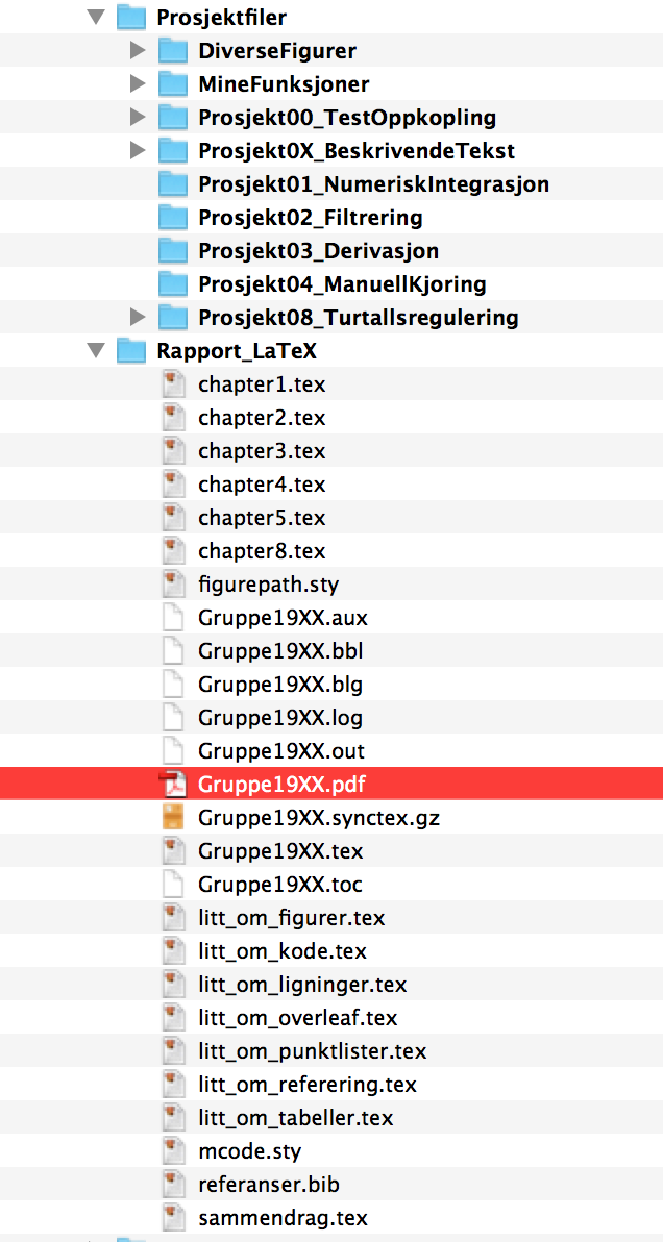
\includegraphics{mappestruktur}}
  \caption{Organisering i mappestruktur hvor {\tt DiverseFigurer}-mappen
    inneholder {\em både} figurer og undermapper med figurer, mens 
    hovedfilen ligger i {\tt Rapport\_LaTeX}-mappen. } 
  \label{fig:mappestruktur}
\end{figure}








\chapter{Litt om Overleaf}\label{kap:overleaf}


Dette kapittelet gir en introduksjon til Overleaf i form av en rekke
skjermdump og beskrivende figurtekster.


\begin{figure}[H]
  \centering
  \scalebox{0.35}{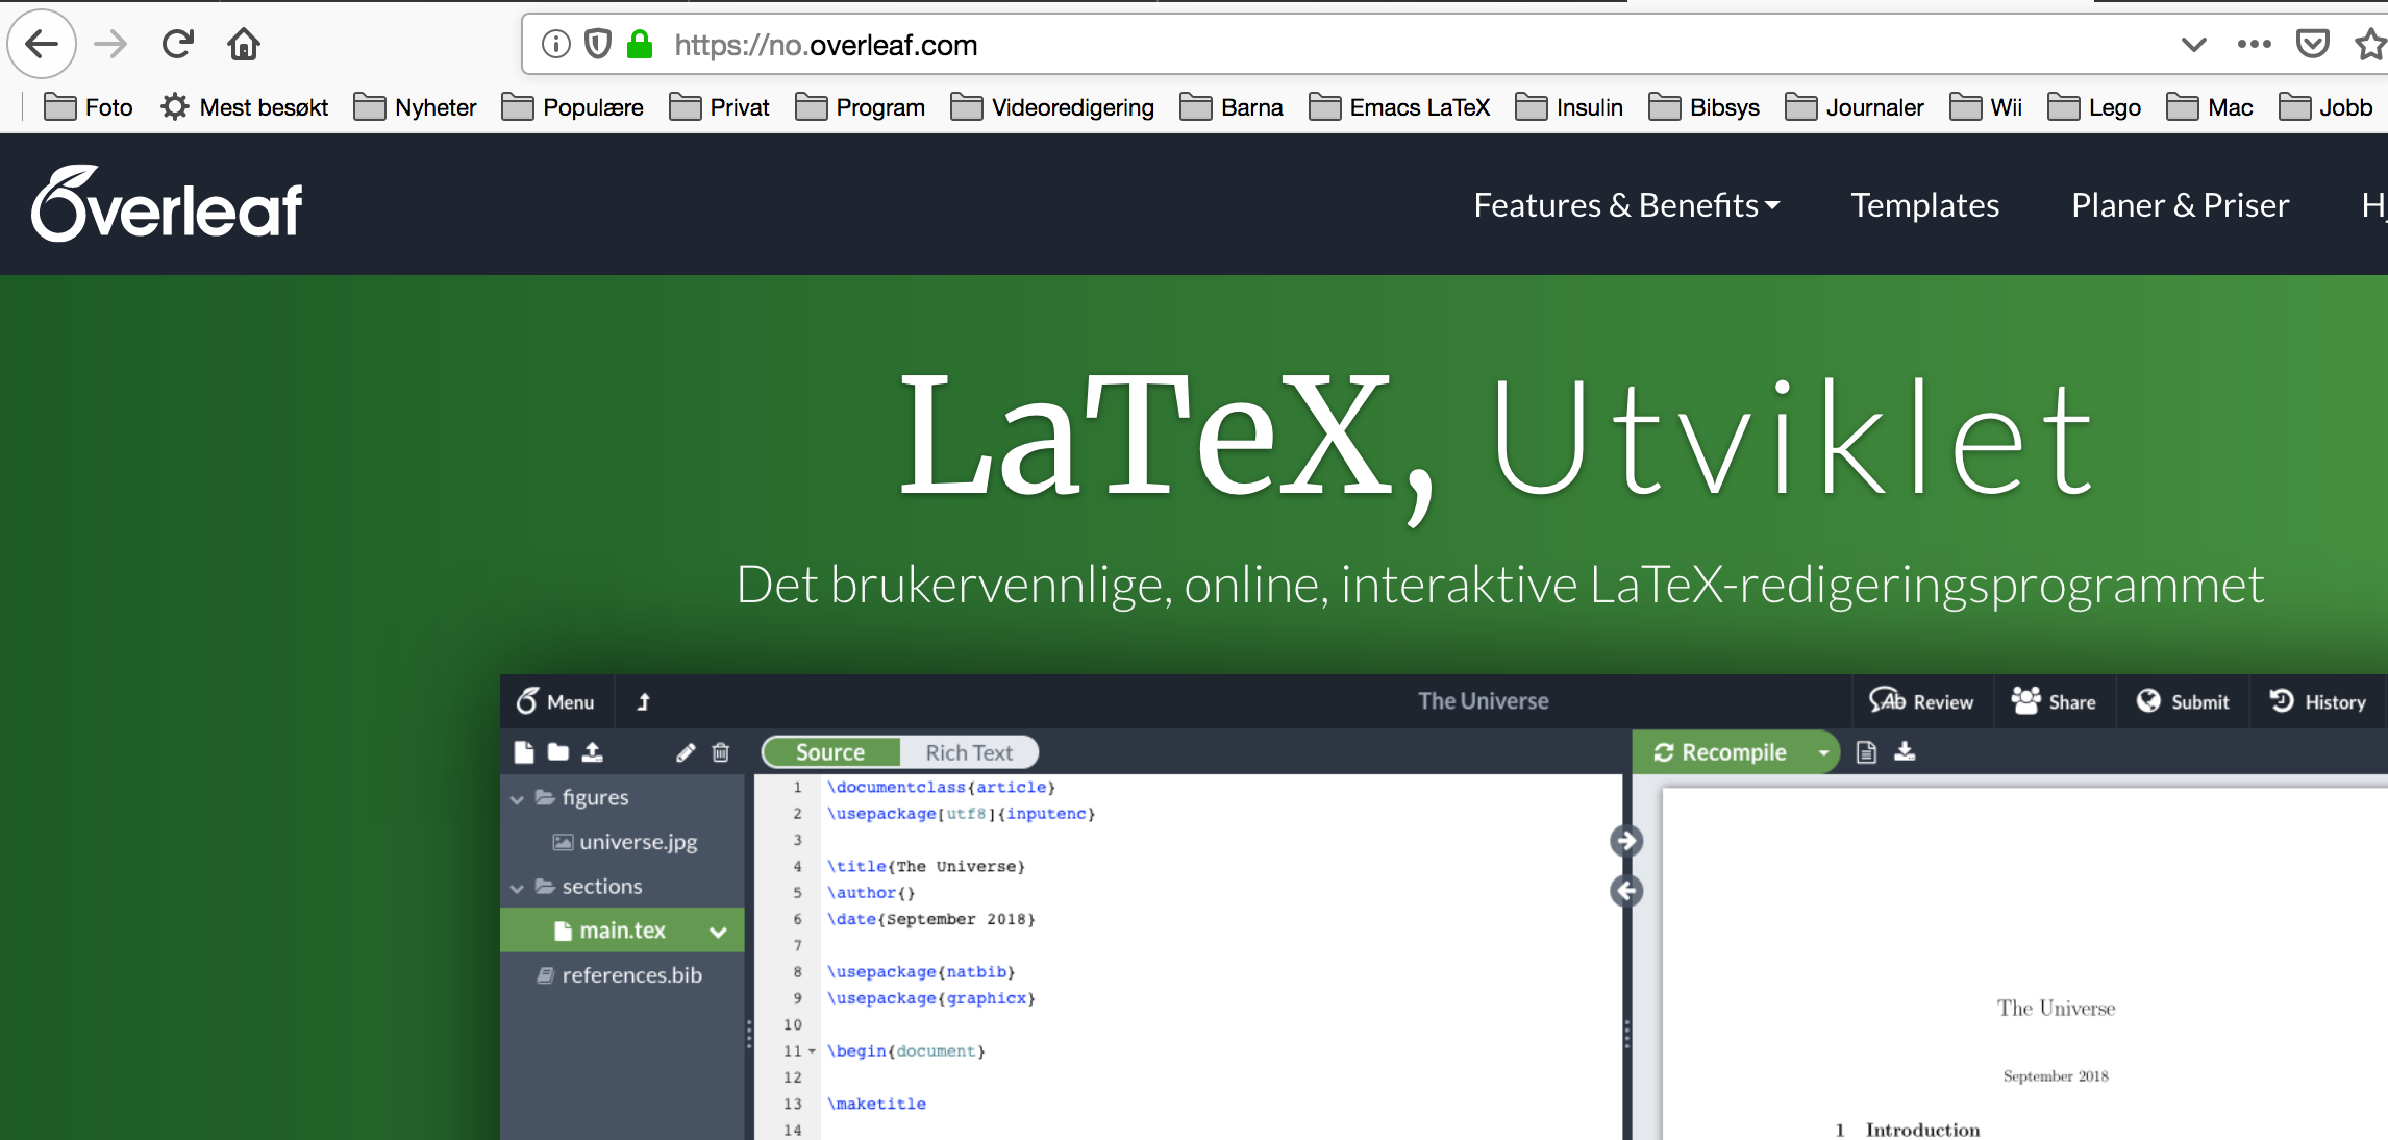
\includegraphics{bilde0}}
  \caption{Gå inn på
    {\color{blue}\href{https://no.overleaf.com/}{https://no.overleaf.com/}}. Registrer
  deg med UiS-epostadressen din. } 
  \label{fig:bilde0}
\end{figure}

\begin{figure}[H]
  \centering
  \scalebox{0.6}{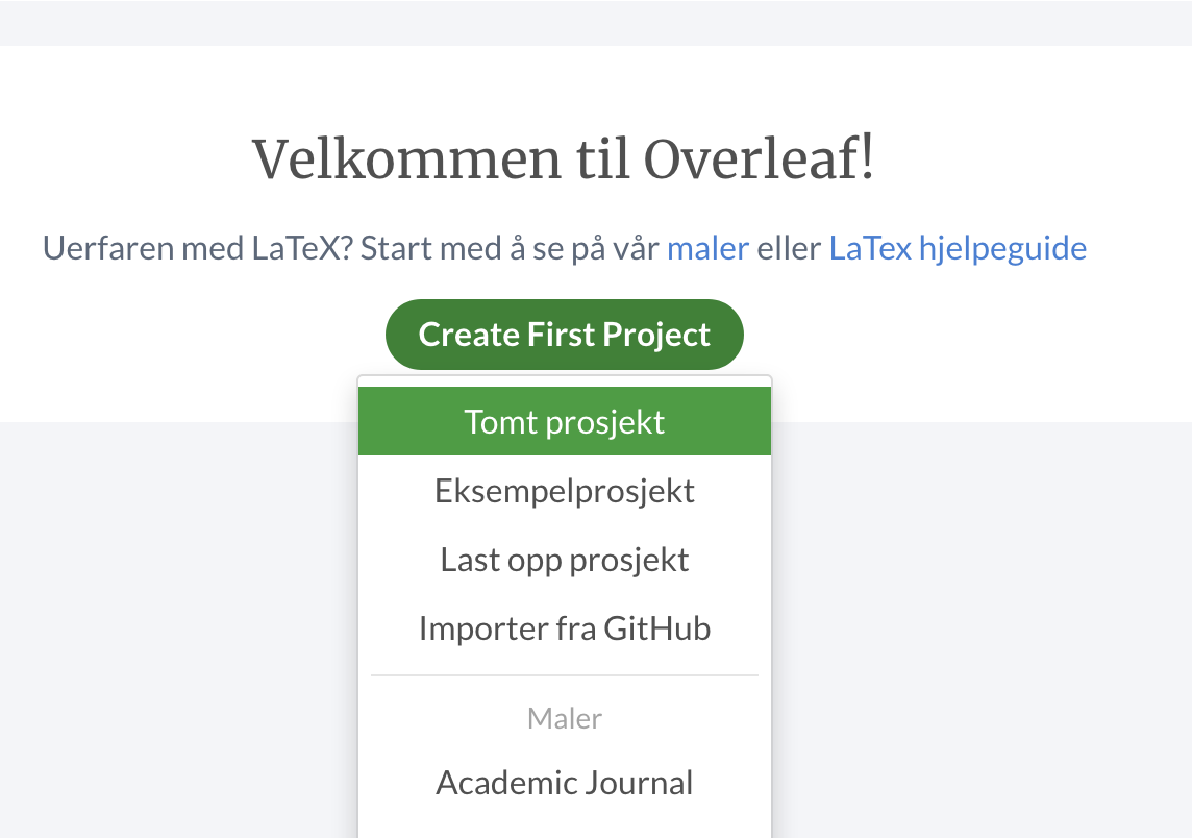
\includegraphics{bilde1}}
  \caption{Etter at du har registrert deg og logget deg inn, trykk på
    ``Create First Project'' og velg ``Tomt prosjekt''.}  
  \label{fig:bilde1}
\end{figure}

\begin{figure}[H]
  \centering
  \scalebox{0.5}{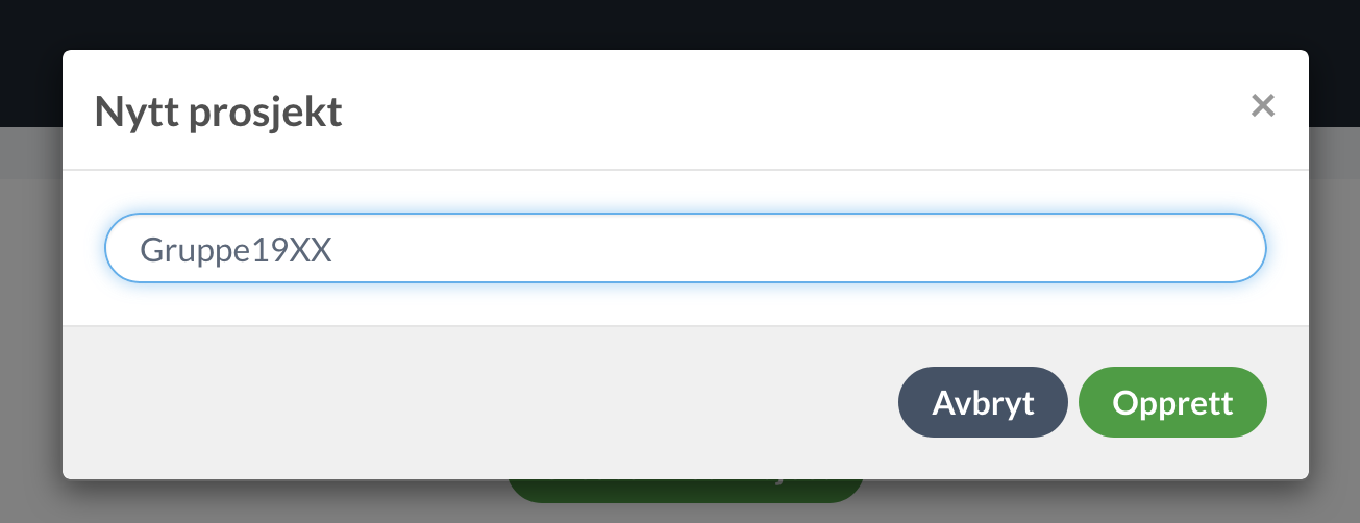
\includegraphics{bilde2}}
  \caption{Kall prosjektet ``Gruppe19XX'' hvor XX er
    gruppernummeret deres.} 
  \label{fig:bilde2}
\end{figure}

\begin{figure}[H]
  \centering
  \scalebox{0.6}{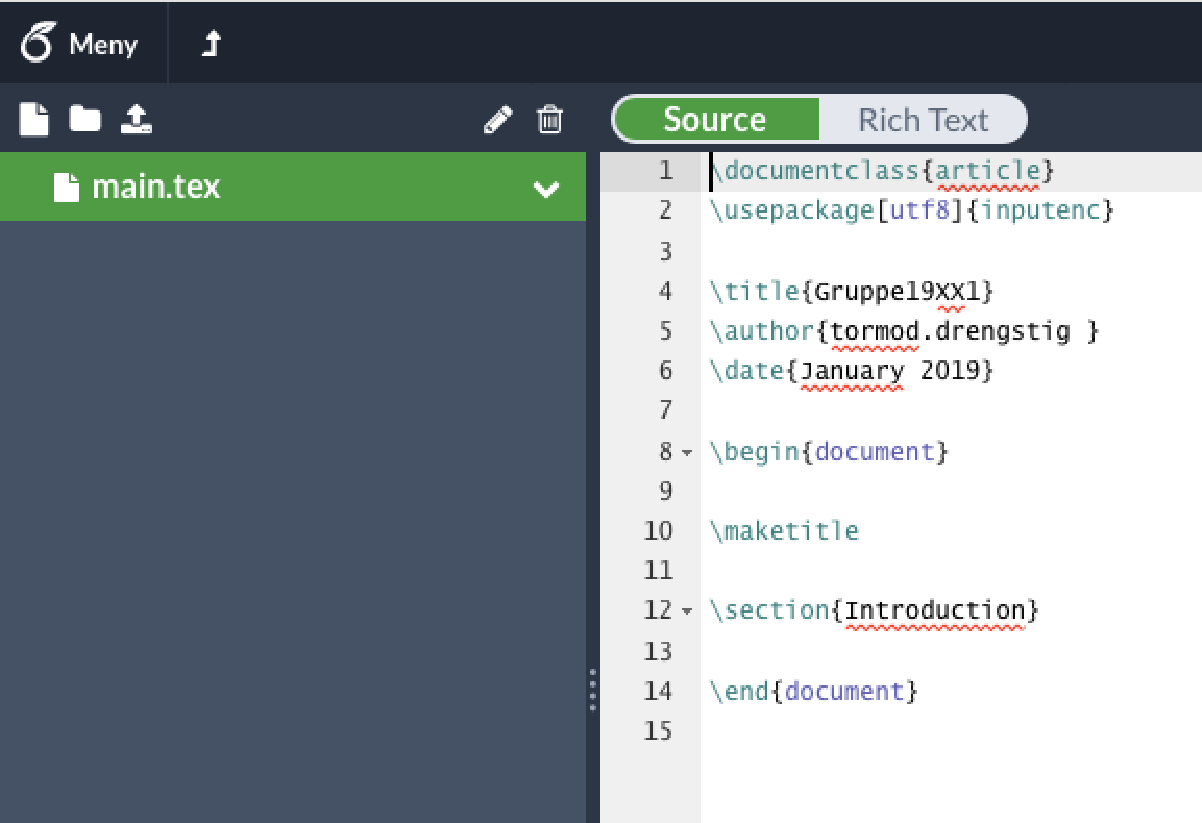
\includegraphics{bilde2a}}
  \caption{Det opprettes automatisk opp en hovedfil kalt 
    \fbox{\tt main.tex} i prosjektet.} 
  \label{fig:bilde2a}
\end{figure}

\begin{figure}[H]
  \centering
  \scalebox{0.8}{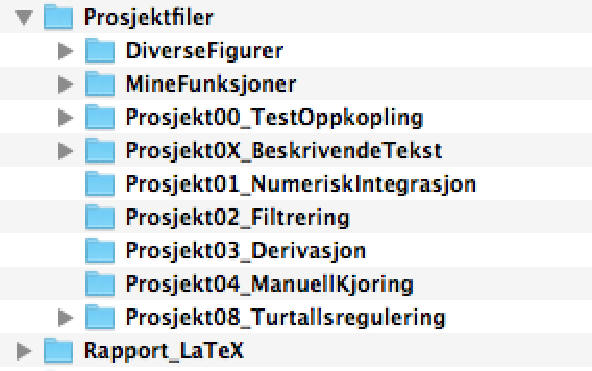
\includegraphics{bilde2b}}
  \caption{Nå er poenget at mappestrukturen som er å finne i {\tt
      Lego.zip}-filen skal lages i Overleaf-prosjektet. Vær klar over
    at det i mappen \fbox{DiverseFigurer} ligger endel figurer samt \fbox{\tt
      overleaf}-mappen. } 
  \label{fig:bilde2b}
\end{figure}

\begin{figure}[H]
  \centering
  \scalebox{0.6}{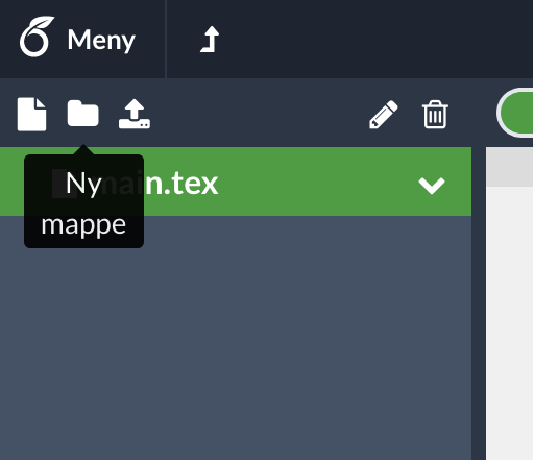
\includegraphics{bilde4}}
  \caption{Trykk på symbolet ``Ny mappe''.} 
  \label{fig:bilde4}
\end{figure}

\begin{figure}[H]
  \centering
  \scalebox{0.6}{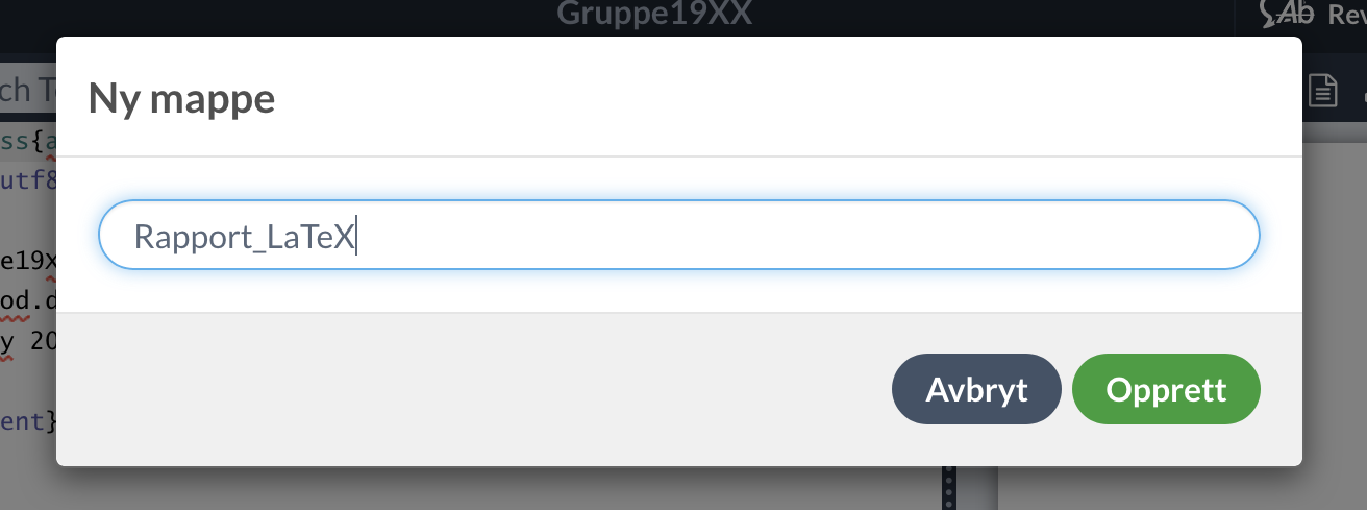
\includegraphics{bilde5}}
  \caption{Lag mappen \fbox{Rapport\_LaTeX}.} 
  \label{fig:bilde5}
\end{figure}


\begin{figure}[H]
  \centering
  \scalebox{0.6}{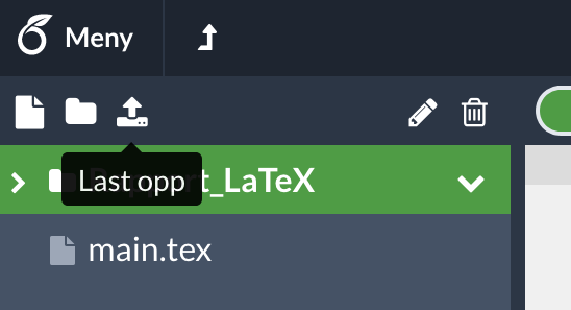
\includegraphics{bilde6}}
  \caption{Stå i mappen \fbox{Rapport\_LaTeX} og trykk ``Last opp''.} 
  \label{fig:bilde6}
\end{figure}


\begin{figure}[H]
  \centering
  \scalebox{0.4}{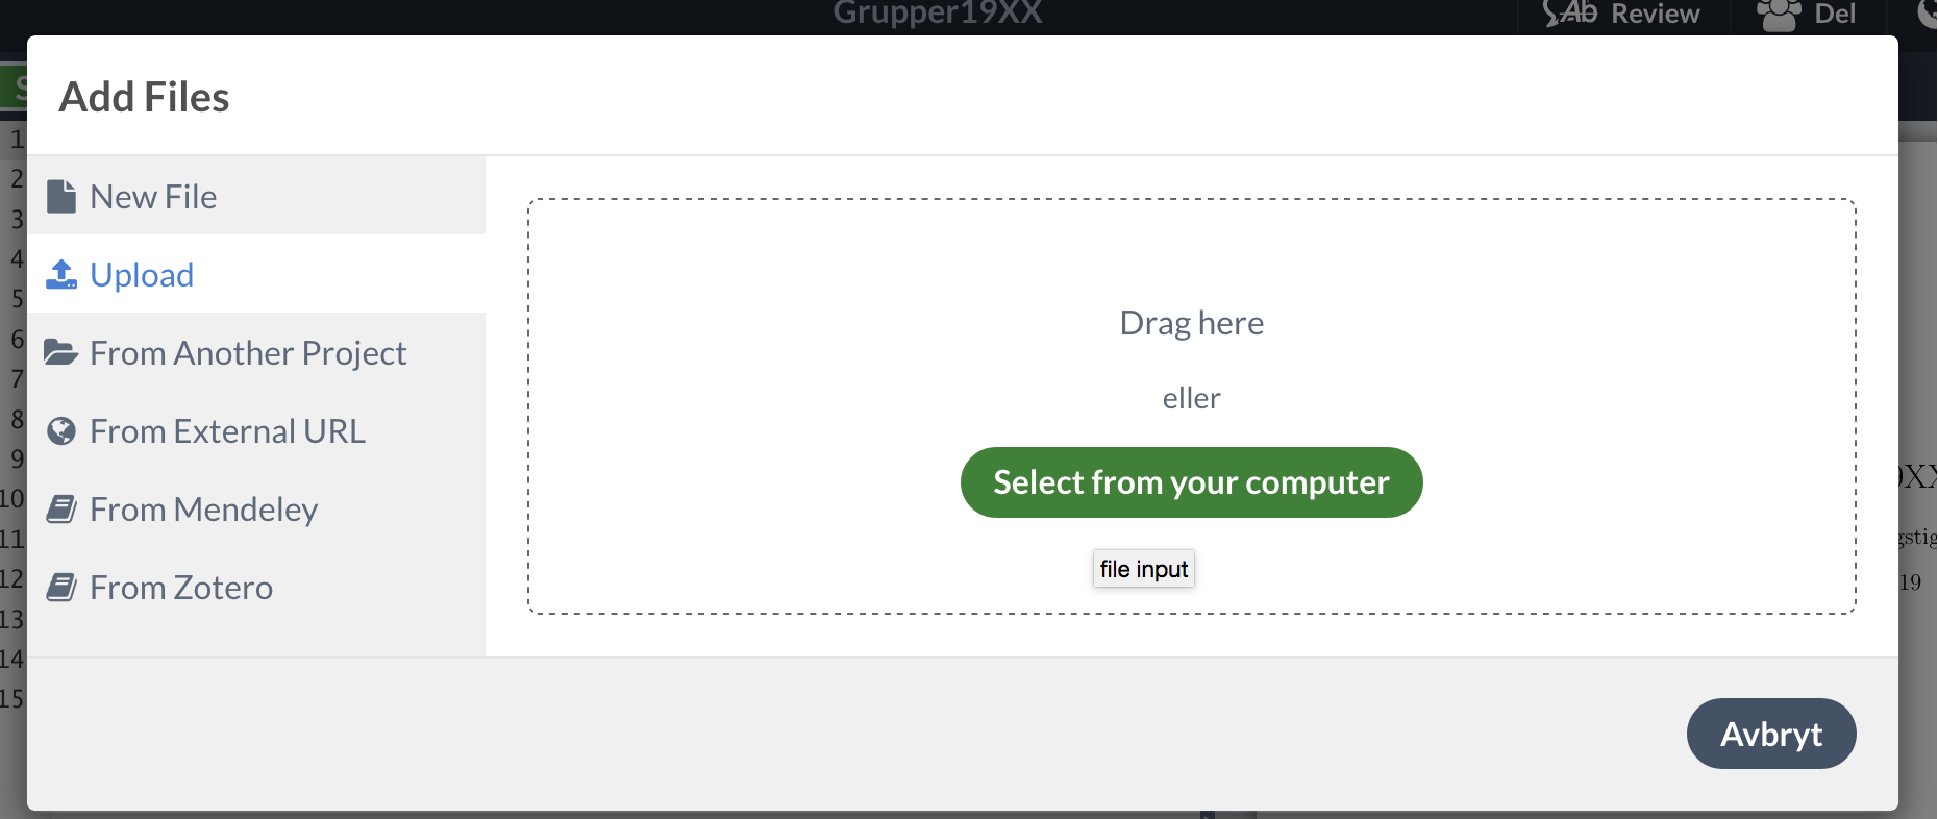
\includegraphics{bilde7}}
  \caption{Trykk på ``Select from your computer''.} 
  \label{fig:bilde7}
\end{figure}

\begin{figure}[H]
  \centering
  \scalebox{0.6}{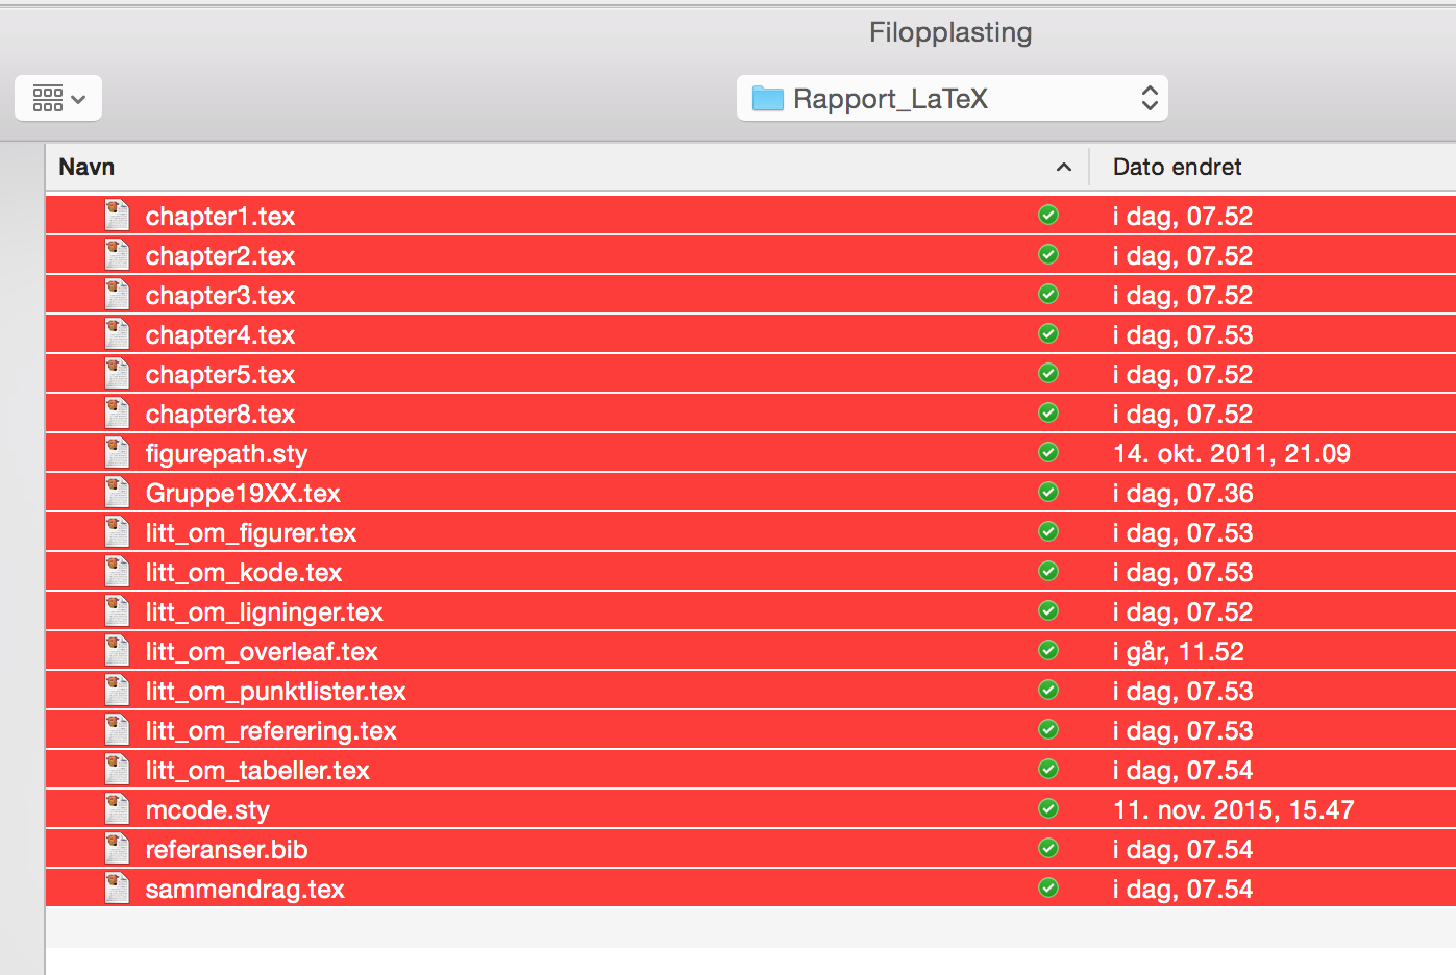
\includegraphics{bilde8}}
  \caption{Naviger deg frem til mappen \fbox{\tt Rapport\_LaTeX} og velg alle filene.} 
  \label{fig:bilde8}
\end{figure}


\begin{figure}[H]
  \centering
  \scalebox{0.4}{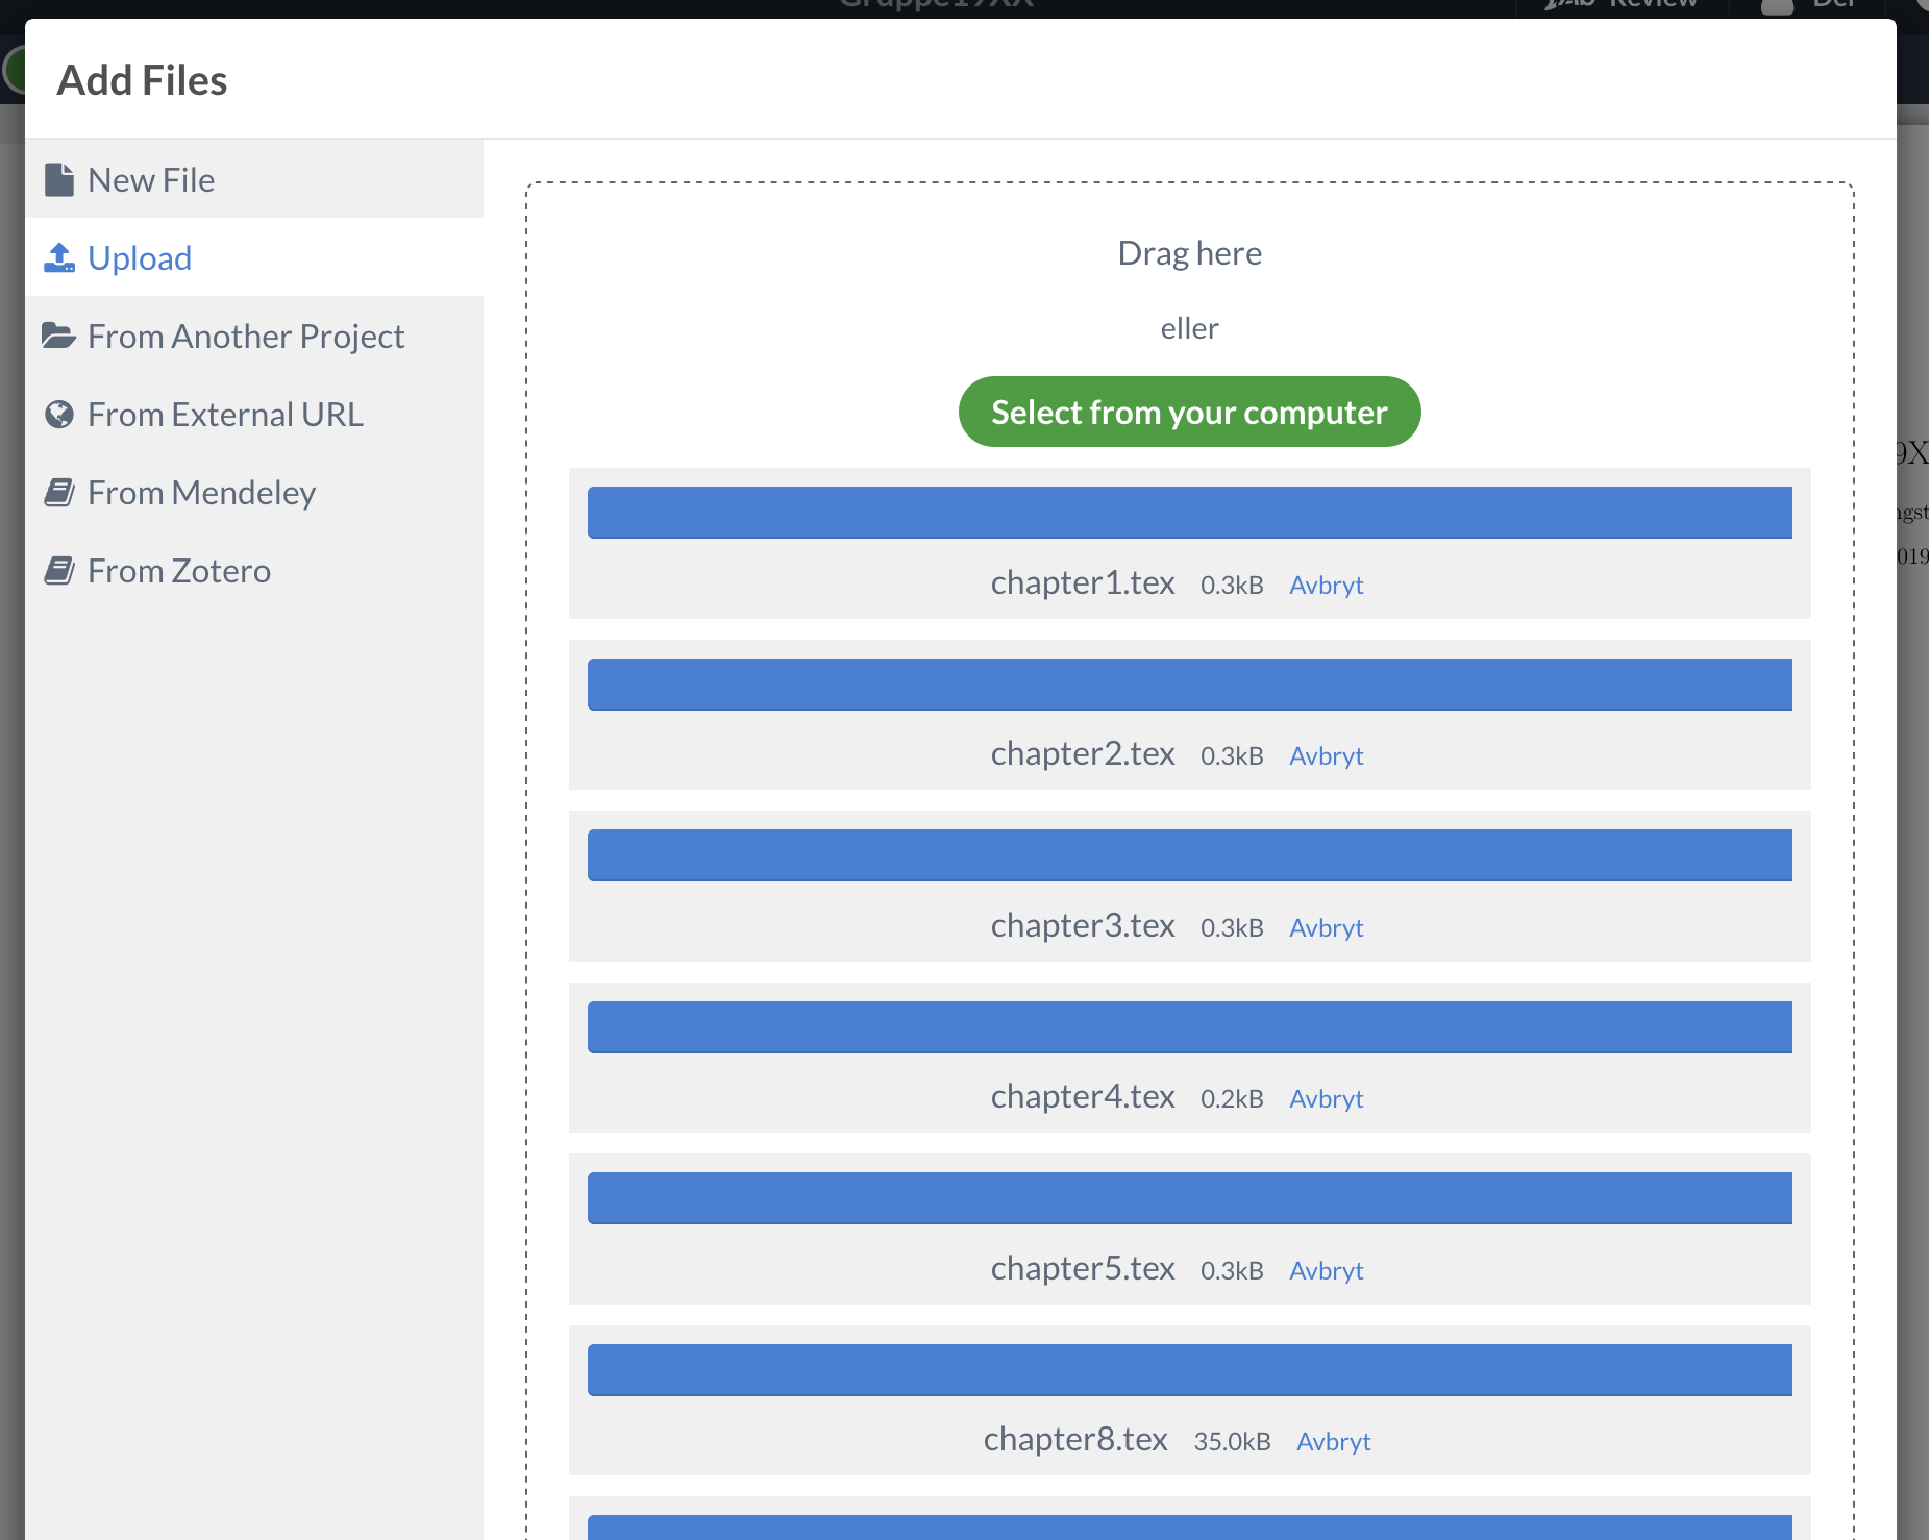
\includegraphics{bilde9}}
  \caption{Filene lastes inn.} 
  \label{fig:bilde9}
\end{figure}


\begin{figure}[H]
  \centering
  \scalebox{0.5}{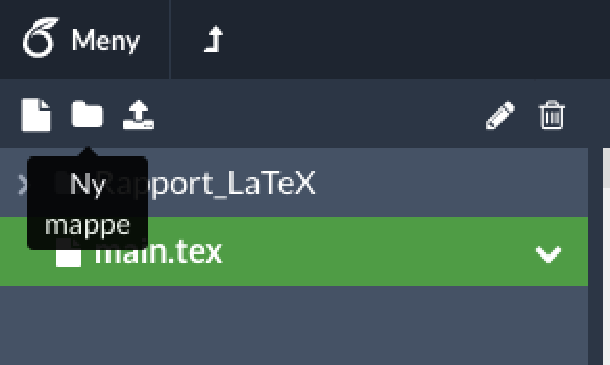
\includegraphics{bilde10}}
  \caption{Stå i filen \fbox{\tt main.tex}, og trykk ``Ny mappe'', og lag
    på samme måte som vist i figur~\ref{fig:bilde5} den nye 
    mappen \fbox{\tt Prosjektfiler}.} 
  \label{fig:bilde10}
\end{figure}

\begin{figure}[H]
  \centering
  \scalebox{0.55}{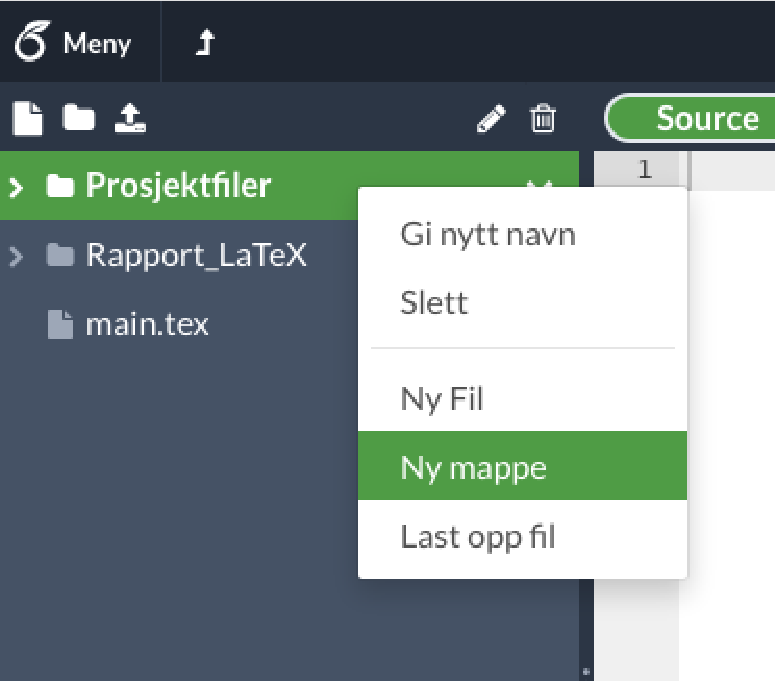
\includegraphics{bilde11}}
  \caption{For å lage undermappene vist i figur~\ref{fig:bilde2b}, 
    stå i mappen \fbox{\tt
      Prosjektfiler}, høyreklikk, og velg ``Ny mappe''. Lag på denne
    måten alle
    mappene som er vist i figur~\ref{fig:bilde12}.} 
  \label{fig:bilde11}
\end{figure}

\begin{figure}[H]
  \centering
  \scalebox{0.55}{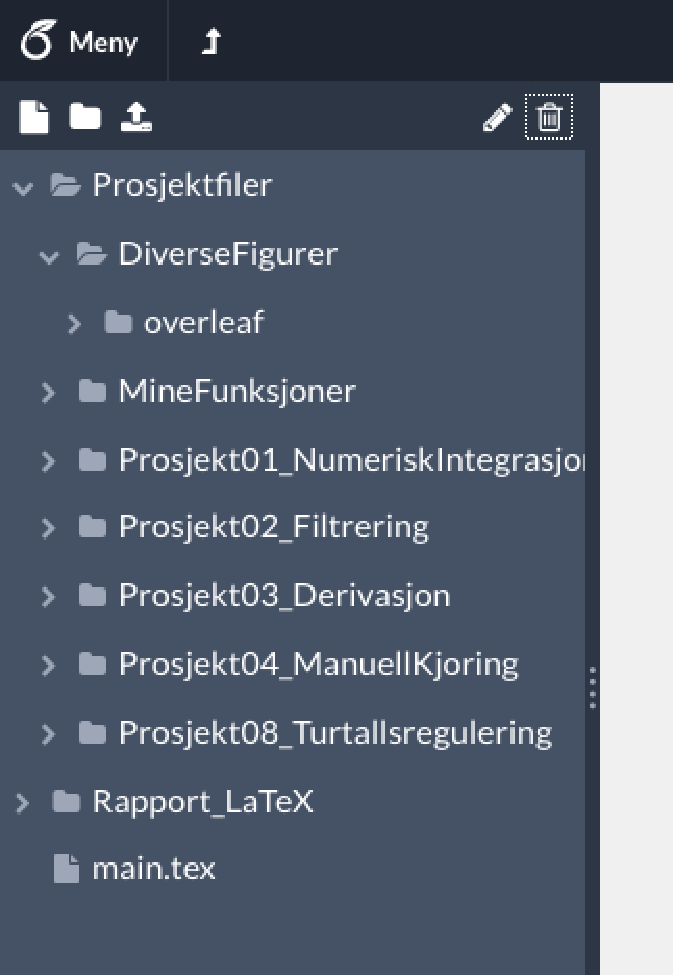
\includegraphics{bilde12}}
  \caption{Mappestrukturen klar.} 
  \label{fig:bilde12}
\end{figure}

\begin{figure}[H]
  \centering
  \scalebox{0.6}{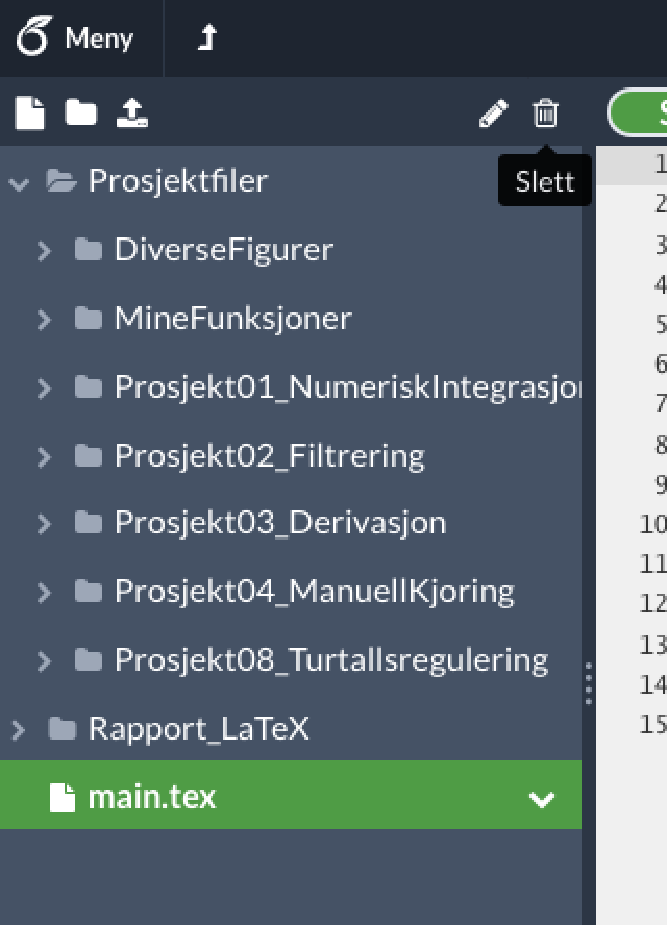
\includegraphics{bilde14}}
  \caption{Slett filen \fbox{\tt main.tex}.} 
  \label{fig:bilde14}
\end{figure}

\begin{figure}[H]
  \centering
  \scalebox{0.7}{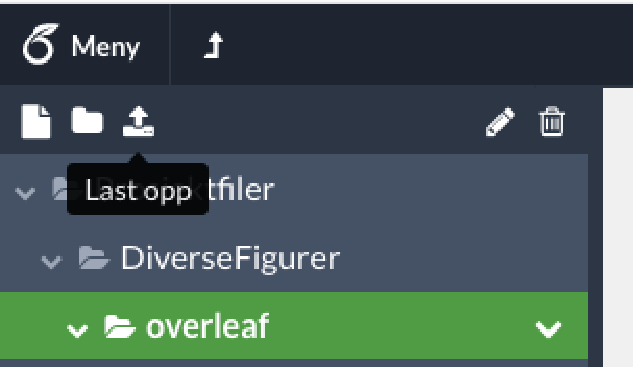
\includegraphics{bilde13}}
  \caption{Nå skal filene i hver mappe lastes inn på samme måte
    som vist i figurene~\ref{fig:bilde6} - \ref{fig:bilde9}. 
    Start f.eks. med å stå i mappen \fbox{\tt overleaf} og trykk ``Last opp''.} 
  \label{fig:bilde13}
\end{figure}

\begin{figure}[H]
  \centering
  \vspace*{-30mm}\scalebox{0.46}{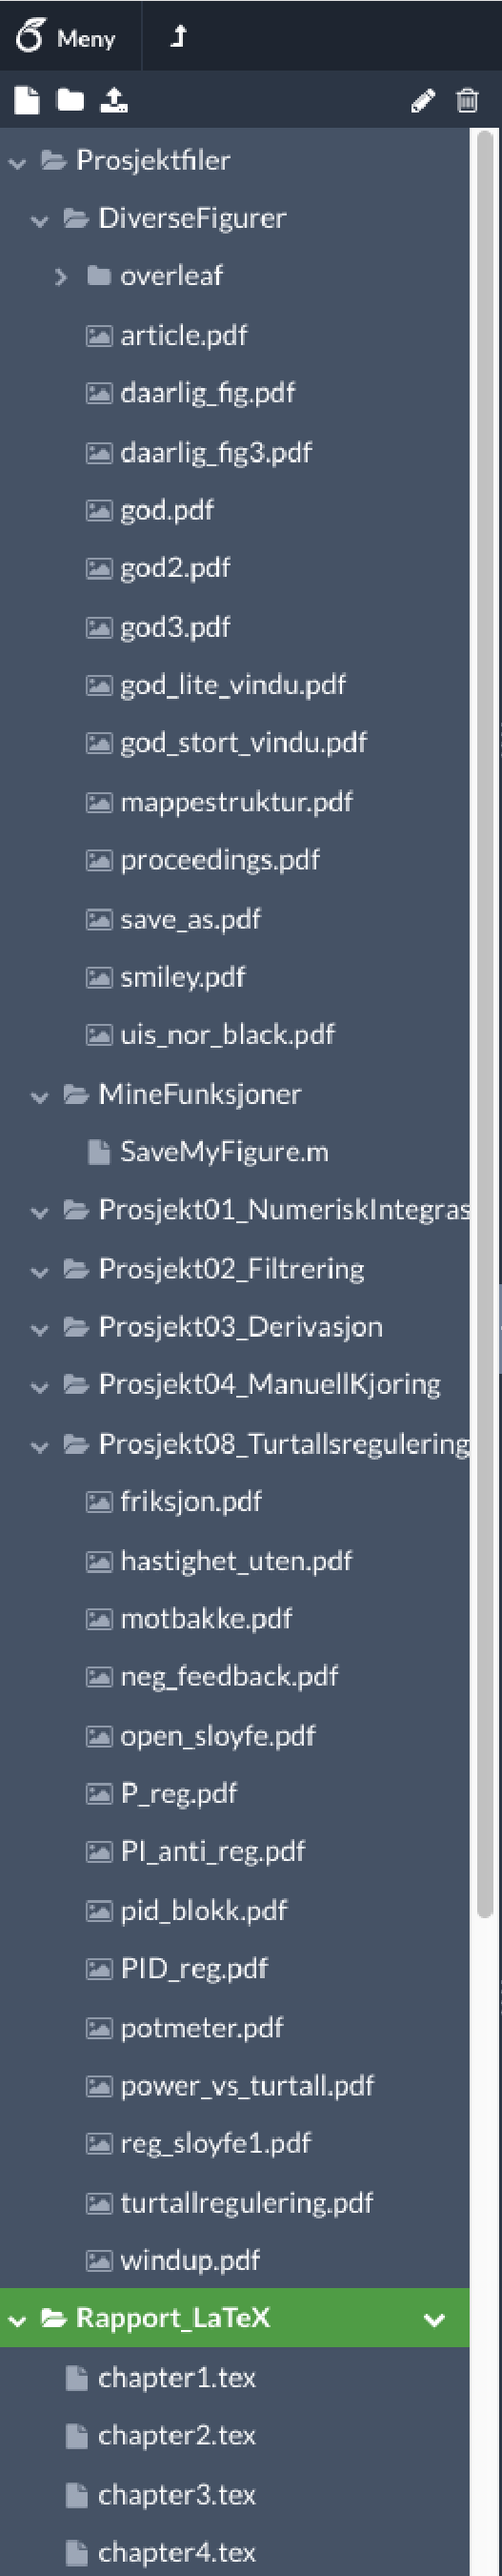
\includegraphics{bilde13a}}
  \caption{Alle filene er på plass. Legg merke til at
    filene i mappen \fbox{\tt overleaf} ikke vises, at mappene
    Prosjekt01... - Prosjekt04... er tomme, samt at det kun er filen {\tt
      SaveMFyFigure.m} som foreløpig ligger i mappen {\tt MineFunksjoner}.} 
  \label{fig:bilde13a}
\end{figure}


\begin{figure}[H]
  \centering
   \hspace*{-30mm}\scalebox{0.6}{\includegraphics{bilde15}}
  \caption{Trykk på \fbox{\tt Gruppe19XX.tex}. Høyreklikk på denne og
    endre navn til gruppenummeret deres.} 
  \label{fig:bilde15}
\end{figure}

\begin{figure}[H]
  \centering
 \scalebox{0.6}{\includegraphics{bilde16}}
  \caption{Trykk på knappen hvor det står ``Rekompiler''. } 
  \label{fig:bilde16}
\end{figure}

\begin{figure}[H]
  \centering
  \scalebox{0.65}{\includegraphics{bilde17}}
  \caption{Etter en stund er den ferdig med å kompilere. Som du ser står det et tall med
    oransje bakgrunn. Det betyr at det er {\em warnings} i
    kompilering. Disse er ufarlige. Dersom bakgrunnen skifter
    farge til {\color{red}rødt} er det kompileringsfeil, og disse må rettes
    opp. Trykk på selve tallet så kommer kompileringsresultatet opp og
    du kan se fra henvisning til linjenummer hvor feilen er.} 
  \label{fig:bilde17}
\end{figure}

\begin{figure}[H]
  \centering
  \scalebox{0.7}{\includegraphics{bilde18}}
  \caption{For å legge til medstudenter i prosjektet, trykk først på
    pilen med knekk for å komme opp til prosjektsiden.} 
  \label{fig:bilde18}
\end{figure}

\begin{figure}[H]
  \centering
  \scalebox{0.6}{\includegraphics{bilde19}}
  \caption{Trykk deretter på ``Konto'' og ``Kontoinnstillinger''.} 
  \label{fig:bilde19}
\end{figure}


\begin{figure}[H]
  \centering
  \scalebox{0.5}{\includegraphics{bilde20}}
  \caption{Trykk på ``Featres \& Benefits'' og så ``For Groups''.} 
  \label{fig:bilde20}
\end{figure}


\begin{figure}[H]
  \centering
  \scalebox{0.5}{\includegraphics{bilde21}}
  \caption{Legg til studenter med sin registrerte epostadresse
    (UiS-adressen). Disclaimer: Jeg er noe usikker på dette
    her siden jeg ikke har hatt mulighet til å teste det ut.} 
  \label{fig:bilde21}
\end{figure}







\chapter{Konklusjon}\label{kap:konklusjon}
Konklusjonen skal generelt være en kort oppsummering av
problemstilling, hva som er gjort og resultatene som er oppnådd.


\bibliographystyle{plain}
\bibliography{referanser.bib}
\addcontentsline{toc}{chapter}{Bibliografi} 

\appendix

\addcontentsline{toc}{chapter}{Vedlegg}
\renewcommand{\appendixname}{Vedlegg}
\renewcommand{\appendixpagename}{Vedlegg}



\chapter{Timelister}\label{ch:vedlegg_A}


\begin{table}[H]
	\centering
	\caption{Timelister for gruppe 19XX i faget ING100.}
              \begin{tabular}{|c|c|c|c|c|c|}\hline
                Navn/uke & Per & Pål 
                &  Anne & Eva\\\hline\hline 
	        40 & & & &  \\\hline
	        41 & & & &  \\\hline
	        42 & & & &  \\\hline
	        43 & & & &  \\\hline
	        44 & & & &  \\\hline
	        45 & & & &  \\\hline
	        46 & & & &  \\\hline\hline
	        Sum & & & &  \\\hline
	\end{tabular}
	\label{tab:timeliste}
\end{table}

\chapter{Programlisting prosjekt 04}\label{ch:vedlegg_B}

\section{P04\_F4\_MathCalculations.m}
\section{P04\_F5\_CalculateAndSetMotorPower.m}

\chapter{Programlisting prosjekt 05}\label{ch:vedlegg_C}
\section{P05\_F4\_MathCalculations.m}
\section{P05\_F5\_CalculateAndSetMotorPower.m}


\end{document}


